\documentclass[11pt,a4paper]{report}
%%%%%%%%%%%%%%%%%%%%%%%%%%%%%%%%%%%%%%%%%%%%%%%%%%%%%%%%%%%%%%%%%%%%%
%%                                                                 %%
%%    Header file for the Phi-S-X Series                           %%
%%                                                                 %%
%%    german version header_gm.tex is derived from header.tex      %%
%%    by uncommenting the line ``\setboolean{german}{true}'' below %%
%%                                                                 %%
%%    Never edit the german version! all changes must be done      %%
%%    in the english version header.tex                            %%
%%                                                                 %%
%%%%%%%%%%%%%%%%%%%%%%%%%%%%%%%%%%%%%%%%%%%%%%%%%%%%%%%%%%%%%%%%%%%%%
%%%%%%%%%%%%%%%%%%%%%%%%%%%%%%%%%%%%%%%%%%%%%%%%%%%%%%%%%%%%%%%%%%%%%
%%                                                                 %%
%%    Header file for the Phi-S-X Series                           %%
%%                                                                 %%
%%    german version header_gm.tex is derived from header.tex      %%
%%    by uncommenting the line ``\setboolean{german}{true}'' below %%
%%                                                                 %%
%%    Never edit the german version! all changes must be done      %%
%%    in the english version header.tex                            %%
%%                                                                 %%
%%%%%%%%%%%%%%%%%%%%%%%%%%%%%%%%%%%%%%%%%%%%%%%%%%%%%%%%%%%%%%%%%%%%%
%====================================================================
%-- define flag for language adaptations
\usepackage{ifthen}   % allows to select only certain text
\provideboolean{german}
\setboolean{german}{false}
%\setboolean{german}{true}  % uncomment this line for german editions
%====================================================================
%
% Textschriftart: Computer modern Bright
% body:            CM-Bright 10pt
% section titles:  CM-Bright Bold
% formulas:        CM-Bright Math Oblique
%
\usepackage[standard-baselineskips]{cmbright}
\usepackage{cmbright}
\usepackage[T1]{fontenc}
\def\usedfonts{CM-Bright}
\usepackage{typearea}
%\typearea[current]{calc} % benutzt die aktuelle 
       % bindekorrektur (BCOR angabe als parameter in koma usepackage)
       % und berechnet satzspiegel neu
\typearea[current]{11} %fixed div value

\usepackage{textcomp} % special symbols
\usepackage{amsfonts} % special symols
                      % see ftp://ftp.ams.org/pub/tex/doc/amsfonts/amsfndoc.pdf
\usepackage{amssymb}  % CM-Bright provides the AMS symbols
\usepackage{exscale}  % allows to scale math expressions to big fonts, 
                      % e.g. \Huge
\usepackage{curves}
\usepackage{braket}
\usepackage{miller}     % miller indices
\usepackage{chemmacros} % http://www.mychemistry.eu/mychemistry/
\usepackage[numbers]{natbib}     % bibliography style
\usepackage{url}\urlstyle{tt}
\usepackage{float}
\usepackage{bm}       % provides the command \bm{} that makes bold math symbols
\usepackage{amsmath}
\usepackage{amsbsy}   % allows bold mathematical symbols
\usepackage{amscd}
 \usepackage{a4wide}  % it is better to use the ``geometry'' package
\usepackage{array}    % 
\usepackage{fancyhdr} %  defines pagestyle fancy
\usepackage{epsfig}   % include graphics with epsfig
\usepackage{graphicx} % includegraphics
\usepackage{epstopdf}
\usepackage{wrapfig}
\usepackage{fancybox} % allows shadow-boxes
\usepackage{color}    % allows to use color in the text
%\usepackage{eepic}
\usepackage{flafter}  % places picture next to its reference
\usepackage{makeidx}  % make an index
%\usepackage{MnSymbol}  % 
%\usepackage{marvosym}  % 
\usepackage{textcase}
\usepackage{ulem} % defines strikeout \sout{}; underline \uline{}
                  % double underline \uuline{}; wave underline \uwave{}
                  % cross out \xout{}
%
%==========================================================================
%==  page layout  =========================================================
%==========================================================================
% eqnarray environment: reduce with of space in place of each ``&''
\setlength\arraycolsep{1.4pt}
\pagestyle{fancy}
%\renewcommand{\chaptermark}[1]{\markboth{\thechapter\ #1}{}}
\renewcommand{\chaptermark}[1]{\markboth{\MakeUppercase{\thechapter\ #1}}{}}
\fancyhf{} 
\fancyhead[LE]{\textsc{\thepage}\qquad\textsc{\leftmark}}
\fancyhead[RO]{\textsc{\leftmark}\qquad\textsc{\thepage}}
\renewcommand{\headrulewidth}{0.5pt}
\renewcommand{\footrulewidth}{0pt} 
\addtolength{\headheight}{2.5pt}
\fancypagestyle{plain}{\fancyhead{}
   \renewcommand{\headrulewidth}{0pt}
   \fancyfoot[CO]{\bfseries\thepage}}

% Line spacing -----------------------------------------------------------
\newlength{\defbaselineskip}
\setlength{\defbaselineskip}{\baselineskip}
\newcommand{\setlinespacing}[1]%
           {\setlength{\baselineskip}{#1 \defbaselineskip}}
\newcommand{\doublespacing}{\setlength{\baselineskip}%
                           {2.0 \defbaselineskip}}
\newcommand{\singlespacing}{\setlength{\baselineskip}{\defbaselineskip}}

% Absatz einr\"ucken ------------------------------------------------------
%\setlength{\parindent}{0pt}
\setlength{\parskip}{2pt}
% -------------------------------------------------------------------------
\ifthenelse{\boolean{german}}
  {\def\figurename{Abb.}}
  {\def\figurename{Fig.}}
%--------------------------------------------------------------------------
\renewcommand{\arraystretch}{1.15}  % skaliert den Zeilen abstand in der 
    % tabular und array umgebung
%
%==========================================================================
%==  boxes etc ============================================================
%==========================================================================
%== minipage in a shadowbox ===============================================
\newenvironment{myshadowminipage}[1]%
  {\par\noindent\begin{Sbox}\begin{minipage}{\linewidth}\vspace{0.1cm}\begin{center}\uppercase{#1}\end{center}}%
  {\vspace{0.1cm}\end{minipage}\end{Sbox}\shadowbox{\TheSbox}}
%
%== minipage in a framedbox ===============================================
\newenvironment{myframedminipage}%
  {\par\noindent\begin{Sbox}\begin{minipage}\linewidth\vspace{0.1cm}}%
  {\vspace{0.1cm}\end{minipage}\end{Sbox}\fbox{\TheSbox}}
%
\newcommand{\myshadowbox}[1]{\noindent\shadowbox{\parbox{\linewidth}{\smallskip #1\smallskip}}}
\newcommand{\myfbox}[1]{\noindent\fbox{\parbox{\linewidth}{\smallskip #1\smallskip}}\medskip}
%== minipage in a framedbox ===============================================
\newtheorem{defi}{Definition}[chapter]
\newenvironment{definition}[1]%
  {\par\noindent\begin{Sbox}\begin{minipage}{\linewidth}\vspace{0.1cm}\begin{defi}\uppercase{#1}\\\vspace{0.1cm}}%
  {\vspace{0.1cm}\end{defi}\end{minipage}\end{Sbox}\shadowbox{\TheSbox}}
%
%=========================================================================
% color used to point out information to the teacher
\definecolor{highlight}{rgb}{1.0,0.7,0.}
\newcommand{\Special}[1]{\textbf{\textcolor{highlight}{#1}}}
%=========================================================================
%  switch certain parts on and off. uses ifthen package
\newboolean{teacher}\setboolean{teacher}{false}
% this parameter can be changed in the manuscript again
\setboolean{teacher}{true} %private version if true!
\newcommand{\teacheronly}[1]{\ifthenelse{\boolean{teacher}}{#1\hfill\\ }}
\newcommand{\editor}[1]{\textcolor{blue}{\texttt{Editor: #1}}}
\newcommand{\MARK}[1]{\textcolor{blue}{#1}} 
\newcommand{\RED}[1]{\textcolor{red}{#1}} 
%
%==========================================================================
%==  define new symbols                                                 ===
%==========================================================================
% define \stat (stationary state) as an operator like \min
\DeclareMathOperator*{\stat}{stat}
\let\Vec=\mathbold   % cmbright.sty provides a bold/italic math alphabet
\let\Dot=\mathbold   % cmbright.sty provides a bold/italic math alphabet
\let\Ddot=\mathbold   % cmbright.sty provides a bold/italic math alphabet
%
\newcommand{\e}[1]{\mathrm{e}^{#1}}% exponential function
\renewcommand{\Re}{\mathrm{Re}}    % real part
\renewcommand{\Im}{\mathrm{Im}}    % imaginary part
\newcommand{\lagr}{\ell}           % Lagrange dichte
\newcommand{\Lagr}{\mathcal{L}}    % Lagrange Funktion
\newcommand{\erf}{{\rm erf}}       %
\newcommand{\atan}{{\rm atan}}     % arcus tangens
\newcommand{\mat}[1]{\bm{#1}}  % Matrix
\newcommand{\gmat}[1]{{\boldsymbol #1}}  % Matrix(symbol)
\newcommand{\defas}{\stackrel{\text{def}}{=}}  %  is defined as
\ifthenelse{\boolean{german}}
  {\newcommand{\rot}{{\rm\bf rot}}}    % curl
  {\newcommand{\rot}{{\rm\bf curl}}}   % curl
\newcommand{\sgn}{{\rm sgn}}       % sign
\ifthenelse{\boolean{german}}
   {\newcommand{\Tr}{\mathrm{Sp}}}      % trace
   {\newcommand{\Tr}{\mathrm{Tr}}}      % trace
\ifthenelse{\boolean{german}}
   {\newcommand{\grmn}[2]{\footnote{``#2'' hei{\ss}t in englisch ``#1''}}}
   {\newcommand{\grmn}[2]{\footnote{``#1'' translates as ``#2'' into German}}}
% define the equation reference
\ifthenelse{\boolean{german}}
   {\newcommand{\eq}[1]{\text{Gl.}~\ref{#1}}}
   {\newcommand{\eq}[1]{\text{Eq.}~\ref{#1}}}
% define a relation with an equation number ontop
\newcommand{\eqrel}[2]{\stackrel{\eq{#1}}{#2}}
\newcommand{\zero}{\varnothing}
%\newcommand{\ket}[1]{|#1\rangle} % contained in package braket
\newcommand{\sumint}{\int\hspace{-15pt}\sum}
\newcommand{\marker}[1]{\textcolor{blue}{\emph{#1}}}
\renewcommand*{\dot}[1]{\overset{\mbox{\large\bfseries .}}{#1}}
\renewcommand*{\ddot}[1]{\overset{\mbox{\large\bfseries\hspace{+0.1ex}.\hspace{-0.1ex}.}}{#1}}
%
%==========================================================================
%==                                                                     ===
%==========================================================================
% Prevent figures from appearing on a page by themselves
% from http://dcwww.camd.dtu.dk/~schiotz/comp/LatexTips/LatexTips.html
\renewcommand{\topfraction}{0.85}
\renewcommand{\textfraction}{0.1}
\renewcommand{\floatpagefraction}{0.75}
%
%==========================================================================
%==                                                                     ===
%==========================================================================
\makeindex    % make index. uses makeidx package.

%== allow links between documents ============================================
\usepackage{xr}
\usepackage{xr-hyper}
%==  hyperref package (must be last package)
\usepackage[colorlinks=true]{hyperref} %specify this as last package
\hypersetup{citecolor=blue}
\hypersetup{menucolor=magenta}
\hypersetup{urlcolor=blue}      % 
\hypersetup{filecolor=green}    % file links
\hypersetup{linkcolor=magenta}  %table of contents
\hypersetup{pdfauthor={Peter E. Bl\"ochl}}
\hypersetup{pdfdisplaydoctitle=true}
\externaldocument[phisx1-]{/Users/ptpb/Tree/PhiSX/ClassicalMechanics/Book/cm-gm}
\externaldocument[phisx2-]{/Users/ptpb/Tree/PhiSX/Electrodynamics/Book/el-gm}
\externaldocument[phisx3-]{/Users/ptpb/Tree/PhiSX/QuantumMechanics/Book/qm}
\externaldocument[phisx4-]{/Users/ptpb/Tree/PhiSX/StatisticalMechanics/Book/sm}
\externaldocument[phisxqm2-]{/Users/ptpb/Tree/PhiSX/QuantumMechanicsII/Book/qm2}
\externaldocument[phisxsm2-]{/Users/ptpb/Tree/PhiSX/StatisticalMechanicsII/Book/sm2}
\externaldocument[phisxcb-]{/Users/ptpb/Tree/PhiSX/Chemicalbond/Book/cb}
% Example: Figure~PhiSX:Quantum
% Mechanics-\ref{phisx3-fig:doubleslitwave} on page
% \pageref{phisx3-fig:doubleslitwave}


\hypersetup{pdftitle=paw_lmto}
\begin{document}
\begin{titlepage}
\begin{center}
\vspace*{3.5cm}
{\huge \textbf{The LMTO object of the CP-PAW code}}\\
\vspace{0.5cm}
{\large Peter E. Bl\"ochl}
\vspace{0.5cm} 
\end{center}

\vfill
\begin{center}
Copyright Peter E. Bl\"ochl; Sept.2, 2013-\today\\
{\small
Institute of Theoretical Physics;
Clausthal University of Technology;\\ 
D-38678 Clausthal Zellerfeld; Germany;\\
http://www.pt.tu-clausthal.de/atp/}
\end{center}
\end{titlepage}
\noindent            
\tableofcontents
%====================================================================
\chapter{Notes}
%====================================================================
%% \begin{itemize}
%% \item The variable \verb|RAUG| must be large enough to enclose the
%%   semi-core states, because the decay of the envelope function is
%%   usually much too slow for them. 
%% %
%% \end{itemize}

%====================================================================
\section{Tests}
%====================================================================
\begin{itemize}
\item is the dynamics energy conserving with fixed positions?
%
\end{itemize}

%====================================================================
\section{Fixes}
%====================================================================
\begin{itemize}
\item lmto\_overlapphi calculates the onsite overlap matrix of partial
  waves in a sphere.
%
\item using only sp like tight-binding orbitals and local exchange
  lead to an increase of the band gap of silicon above 1.3 eV. After
  adding the d-orbitals to the HF term collapsed the band gap
  dramatically below the dft value. Core-valence echange seems to have
  an important effect on the band gap too.
%
%% \item double counting in \verb|paw_lmto| and \verb|paw_dmft| is in
%%   error. It takes the partial wave density matrix do do it
%%   properly. currently only the density of AEF is used.

%%   Double counting fixed before Nov. 13, 2014 (Commit 106f8a0). Both
%%   versions of double counting can be addressed by a hard-wired switch.
%
\item The charge sumrule is not correct! The calculation for an H-atom
  yields $Tr[\rho O]\approx 0.2$. The problem is not the difference
  between tailed orbitals and the multicenter expansion, because
  $(r*\chi)^2$ agrees quire well.
%
\end{itemize}


%====================================================================
\section{Ideas and remarks}
%====================================================================

%====================================================================
\chapter{Purpose and theoretical background of the LMTO Object}
%====================================================================
The LMTO object maps the wave functions expressed in augmented plane
waves onto a basiset of \textbf{natural tight-binding
  orbitals}\index{natural tight-binding orbitals}. The natural
tight-binding orbitals are a kind of LMTO's, screened such that the
tails exhibit only scattering character in the context of nodeless
wave functions\cite{bloechl12_arxiv1210_5937}.

%====================================================================
\section{Augmentation: Overview}
%====================================================================
The concept of linear augmented waves\cite{andersen75_prb12_3060} is
as follows:
\begin{enumerate}
\item At first, a so-called \textbf{envelope function}\index{envelope
  function} $|K^\infty_\alpha\rangle$ is defined.\footnote{The
  superscript $\infty$ denotes that the function extends over all
  space, a superscript $\Omega$ denotes that the function is truncated
  (set to zero) outside the augmentation sphere $\Omega_{R}$ centered
  at the site $R_\alpha$ denoted by the index $\alpha$. The
  superscript $I$ denotes that the function is non-zero only in the
  interstitial region, that is outside all augmentation spheres. If
  the augmentation spheres overlap, the function in the interstitial
  region is defined by subtraction of all sphere
  contributions. Similarly, the interstitial function constains terms
  from the higher angular momenta within the augmentation regions.}
%
\item In a second step, this envelope function is expanded about each
  atomic site $R_\alpha$ into spherical harmonics.  More generally,
  they are expanded into \textbf{head functions}\index{head function}
  $|K^\Omega_\alpha\rangle$ and \textbf{tail functions}\index{tail
    function} $|J^\Omega_\alpha\rangle$. The head function is the
  dominant contribution and carries the quantum number of the final
  orbital, while the tail functions are the minor contributions with
  different quantum numbers. In practice, the head functions are solid
  Hankel functions and the tail functions are solid Bessel functions.
\begin{eqnarray}
|K_{\alpha}^\infty\rangle=|K^\Omega_{\alpha}\rangle
-\sum_{\beta}|J^\Omega_{\beta}\rangle S^\dagger_{\beta,\alpha}
+|K^I_{\alpha}\rangle
\label{eq:multicenterexpandenvelopefunction1}
\end{eqnarray}
   The coefficients $S_{\alpha,\beta}$ of the tail functions are
   called \textbf{structure constants}\index{structure constants}.

  The difference between the full envelope function and its expansion
  into head and tail functions is the \textbf{interstitial envelope
    function}\index{interstitial envelope function}\footnote{The
    interstitial envelope function is confined mostly in the region in
    between the atoms, but it also accounts for the overlap of the
    atomic regions and so-called higher partial waves not taken care of
    in the regular partial-wave expansion.}  $|K^I_\alpha\rangle$.
%
\item In the third step, the head and tail functions are replaced
  differentiably at some sphere radius by \textbf{partial
    waves}\index{partial waves} of the atomic potential. For that
  purpose, we use as partial waves a solution of the Schr\"odinger
  equation for some energy, denoted as $|\phi_{\alpha}\rangle$ and its
  energy derivative function $|\dot{\phi}_\alpha\rangle$.

  The matching parameters are called \textbf{potential
    parameters}\index{potential parameters}.
\end{enumerate}

%====================================================================
\section{Envelope functions and structure constants}
%====================================================================
%====================================================================
\subsection{Hankel functions as envelope function}
%====================================================================
In practice, we will use solid Hankel functions $H_L(\vec{r})$ as
envelope functions, so that 
\begin{eqnarray}
\langle\vec{r}|K^\infty_\alpha\rangle= H_{L_\alpha}(\vec{r}-\vec{R}_\alpha)
\end{eqnarray}


Solid Hankel functions are irregular solutions of the the
inhomogeneous Helmholtz equation\footnote{I am not sure whether also
  the three dimensional differential equation or only the
  one-dimensional differential equation for the radial part is called
  Helmholtz equation.}
\begin{eqnarray}
\Bigl[\vec{\nabla^2}+k^2\Bigr]H_{L}(\vec{r})
=-4\pi(-1)^\ell\mathcal{Y}(\vec{\nabla})\delta(\vec{r})
\label{eq:solidhelmholtzequation}
\end{eqnarray}
Here $\mathcal{Y}_L(\vec{r})\defas r^\ell Y_L(\vec{r})$ is a
polynomial. With a gradient as argument, it becomes a differential
operator. With $Y_L(\vec{r})$ we denote a spherical or real harmonic
function and $L\defas(\ell,m)$ is a composite index of angular
momentum quantum number $\ell$ and magnetic quantum number $m$.

Further details about the Hankel and Bessel functions can be found in
appendix~\ref{app:solidhankel}.

%====================================================================
\subsection{Hankel and Bessel functions as head and tail functions}
%====================================================================
Defining the envelope function via an isotropic and translationally
invariant differential equation of second order has the advantage
that the solution can be expanded about different centers into regular
solutions of the same differential equation with specific angular
momenta. The regular solutions of the Helmholtz equation are the
Bessel functions.

Hankel and Bessel functions are defined\footnote{This is our
  definition, not a generally accepted convention.} so that they
behave at the origin as
\begin{eqnarray}
K^\Omega_{R,L}(\vec{r})&=&
\Bigl[(2\ell-1)!! \frac{1}{|\vec{r}-\vec{R}|^{\ell+1}} 
+...\Bigr]
Y_L(\vec{r}-\vec{R})\theta_{\Omega_R}(\vec{r})
\\
J^\Omega_{R,L}(\vec{r})&=&
\biggl[\frac{1}{(2\ell+1)!!} |\vec{r}-\vec{R}|^{\ell+1} 
+...\Bigr]Y_L(\vec{r}-\vec{R})\theta_{\Omega_R}(\vec{r})
\end{eqnarray}
$\theta_{\Omega_R}(\vec{r})$ is a step function, which equals unity within the
augmentation region $\Omega_R$ centered at site $R$, while it vanishes
outside. The terms neglected are higher orders in $|\vec{r}-\vec{R}|$.

%====================================================================
\subsection{Bare structure constants}
%====================================================================
The \textbf{bare structure constants}\index{structure constants !bare}
$S^\dagger_{\beta,\alpha}$ are the expansion constants for an
off-center expansion of solid spherical Hankel functions\index{Hankel
  function} $|K_{\alpha}^\infty\rangle$ into \textbf{solid Bessel
  functions}\index{Bessel function} $|J^\Omega_{\beta}\rangle$.
\begin{eqnarray}
|K_{\alpha}^\infty\rangle=|K^\Omega_{\alpha}\rangle
-\sum_{\beta}|J^\Omega_{\beta}\rangle S^\dagger_{\beta,\alpha}
+|K^I_{\alpha}\rangle
\end{eqnarray}
The index $\alpha$ denotes here an atomic site $R$ and a set of
angular momenta $L=(\ell,m)$.

The superscript $\infty$ denotes that the function extends over all
space, a superscript $\Omega$ denotes that the function is truncated
(set to zero) outside the augmentation sphere $\Omega_{R}$ centered at
the site denoted by the index. The superscript $I$ denotes that the
function is limited to the interstitial region, that is, outside all
augmentation spheres. If the augmentation spheres overlap, the
function in the interstitial region is defined by subtraction of all
sphere contributions.



\begin{myshadowminipage}{Bare structure constants}
The bare structure constants have the form
\begin{eqnarray}
S_{RL,R'L'}=(-1)^{\ell'+1} 4\pi \sum_{L''} C_{L,L',L''} 
H_{L''}(\vec{R}'-\vec{R})
\begin{cases}
(-ik)^{\ell+\ell'-\ell''}&\text{for $k^2>0$}\\
\delta_{\ell+\ell'-\ell''}&\text{for $k^2=0$}\\
\kappa^{\ell+\ell'-\ell''}&\text{for $k^2=-\kappa^2<0$}\\
\end{cases}
\label{eq:fortmulaforbarestructureconstants}
\end{eqnarray}
\end{myshadowminipage}

With $C_{L,L',L''}$, we denote the \textbf{Gaunt
  coefficients}\index{Gaunt coeffocients} defined by
\begin{eqnarray}
Y_{L'}(\vec{r})Y_{L''}(\vec{r})=\sum_L Y_{L}(\vec{r})C_{L,L',L''}
\end{eqnarray}
Note, that the Gaunt coefficients for spherical and real spherical
harmonics differ.\footnote{In practice, we use real spherical
  harmonics and the corresponding Gaunt coefficients.}

The bare structure constants are hermitean\footnote{We use that
  $H_L(\vec{r})=(-1)^\ell H_L(-\vec{r})$ and that the Gaunt
  coefficients $C_{L,L',L''}$ vanish unless $\ell+\ell'+\l''$ is
  even.}, i.e.
\begin{eqnarray}
S_{RL,R'L'}=S_{R'L',RL}
\end{eqnarray}
This is, however, not true for each angular-momentum block individually,
i.e. in general we have $S_{RL,R'L'}\neq S_{R,L',R'L}$.



%====================================================================
\subsection{Gradient of structure constants}
%====================================================================

See P. Bl\"ochl, Methods: chapter \textit{Working with spherical harmonics},
Section \textit{Gradients of spherical harmonics}.
\begin{eqnarray}
\partial_{r_j} Y_L(\vec{r})=\sqrt{\frac{4\pi}{3}}\sum_{L'}
C_{p_j,L,L'}\left[\frac{-\ell}{r}+\frac{2\ell+1}{r}\delta_{\ell',\ell-1}
\right]Y_{L'}(\vec{r})
\end{eqnarray}


For the product of a radial function $f(|\vec{r}|)$ and a spherical 
harmonics, I obtain
\begin{eqnarray}
\partial_{r_j}\Bigl[f(|\vec{r}|) Y_L(\vec{r})\Bigr]
=\sqrt{\frac{4\pi}{3}}\sum_{L'}
C_{p_j,L,L'}
\left[
\frac{-\ell}{r}+\frac{2\ell+1}{r}\delta_{\ell',\ell-1}
+\left.\partial_r\right|_{r=\sqrt{\vec{r}^2}} 
\right]
f(|\vec{r}|)Y_{L'}(\vec{r})
\end{eqnarray}

I used
\begin{eqnarray}
  Y_{p_j}(\vec{r})=\sqrt{\frac{3}{4\pi}}\frac{r_j}{|\vec{r}|}
\end{eqnarray}

%====================================================================
\section{Augmentation and Potential parameters}
%====================================================================
%=======================================================================
\subsection{Local orbitals}
%=======================================================================
Local orbitals are augmented Hankelfunctions
\begin{eqnarray}
|\chi_\gamma\rangle&=&
\sum_\alpha \biggl\lbrace
\underbrace{
|\phi^{K}_{\alpha}\rangle+ |K^{\notin\Omega_\alpha}_\alpha\rangle
}_{\text{R-independent}}
\underbrace{
-\sum_{\beta}
\biggl(|\phi^J_{\beta}\rangle -|J_{\beta}\rangle\biggr)
S^\dagger_{R_\beta,L_\beta,R_\alpha,L_\alpha}}_{\text{R-dependent and small}}
\biggr\rbrace c_{\alpha,\gamma}
\nonumber\\
&=&\sum_\alpha \biggl\lbrace
|\phi^{K}_{\alpha}\rangle
-\sum_{\beta}
|\phi^J_{\beta}\rangle S^\dagger_{R_\beta,L_\beta,R_\alpha,L_\alpha}
+ |K^{I}_\alpha\rangle
\biggr\rbrace c_{\alpha,\gamma}
\end{eqnarray}
Here, $|\phi^K_\alpha\rangle$ is a superposition of partial waves,
which match at the augmentation radius to $|K_\alpha\rangle$, and
which are set to zero outside the augmentation region.
$|K^{\notin\Omega_\alpha}_\alpha\rangle$ is the Hankelfunction at site
$R_\alpha$ and angular momentum $L_\alpha$, which is set to zero
inside its central augmentation region $\Omega_\alpha$.

The interstitial envelope function, which is zero in all augmentation
regions is (see also \eq{eq:multicenterexpandenvelopefunction1})
\begin{eqnarray}
|K^I_\alpha\rangle= |K^{\notin\Omega_\alpha}_\alpha\rangle
-\sum_{\beta}|J_{\beta}\rangle
S^\dagger_{R_\beta,L_\beta,R_\alpha,L_\alpha}
\end{eqnarray}


A suitable definition for $\mat{c}$ is a matrix that produces
orthonormal states for an isolated atom. Thus, it is an onsite matrix.
It is constructed by a onsite-Gram-Schmidt decomposition.

We introduce head and tail functions defined as
\begin{eqnarray}
|\phi^H_\alpha\rangle&=&\sum_{\beta; R_\beta=R_\alpha}
|\phi^K_\beta\rangle c_{\beta,\alpha}
\nonumber\\
|\phi^T_\alpha\rangle&=&|\phi^J_\alpha\rangle
\end{eqnarray}
so that
\begin{eqnarray}
|\chi_\gamma\rangle&=&
|\phi^{H}_{\gamma}\rangle
-\sum_{\alpha,\beta}
|\phi^J_{\beta}\rangle S^\dagger_{R_\beta,L_\beta,R_\alpha,L_\alpha}
c_{\alpha,\gamma}
+\sum_\alpha |K^{I}_\alpha\rangle c_{\alpha,\gamma}
\end{eqnarray}



%===============================================================================
\subsection{Partial waves}
%===============================================================================
The partial waves are constructed using the nodeless (or node
reduced?) construction. 

\begin{enumerate}
\item The node-reduced partial waves are matched to the envelope
  function.
\item the all-electron and pseudo local orbitals are constructed by
  adding and subtracting the difference of the corresponding partial
  wave minus the node-reduced partial waves. This construction allows
  the all-electron and pseudo orbitals to deviate from the envelope
  functuion also beyond the augmentation region.
\end{enumerate}




%===============================================================================
\subsection{Matching}
%===============================================================================
The new partial waves $|\phi^K_\alpha\rangle$ and
$|\phi^{\bar{J}}_\alpha\rangle$ are superpositions of the valence and
scattering partial waves that match differentiably to the head and
tail functions $|K_\alpha\rangle$ and $|J_\alpha\rangle$.
\begin{eqnarray}
|K_\alpha\rangle\rightarrow
|\phi^K_\alpha\rangle&=&
\overbrace{
|\phi_\alpha\rangle 
\underbrace{
\frac{W_\alpha[K,\dot{\phi}]}{W_\alpha[\phi,\dot{\phi}]}}_{Ktophi}
-\,|\dot{\phi}_\alpha\rangle 
\underbrace{\frac{W_\alpha[K,\phi]}{W_\alpha[\phi,\dot{\phi}]}}_{-Ktophidot}
}^{\rightarrow |K^\Omega_\alpha\rangle}
\nonumber\\
|\phi^{J}_{R,L}\rangle
&=&\overbrace{
|\dot{\phi}_\beta\rangle 
\underbrace{\biggl(-\frac{W_\beta[J,\phi]}{W_\beta[\phi,\dot{\phi}]}\biggr)}_{JBARtophidot}
}^{\rightarrow |J\;^\Omega_\beta\rangle}
\end{eqnarray}
Note, that in the factor $JBARTOPHIDOT$ does not depend on the choice
of $|\phi\rangle$.

With $W_\alpha[f,g]$ we denote the \textbf{Wronskian}\index{Wronskian}
\begin{eqnarray}
W_\alpha[f,g]\defas f_\alpha (\partial_r g_\alpha)-(\partial_r f_\alpha)g_\alpha
=\det\left[\begin{array}{cc}f&g\\\partial_rf&\partial_rg\end{array}\right]
\end{eqnarray}
which is used to match two functions differentiably to a third via
\begin{eqnarray}
y(x)\rightarrow f(x)\frac{W[y,g]}{W[f,g]}+g(x)\frac{W[y,f]}{W[g,f]}
\end{eqnarray}


The matrix elements
$\langle\tilde{p}_\gamma|\tilde{\chi}_\alpha\rangle$, which will be
needed later, have the form
\begin{eqnarray}
\langle\tilde{p}_\gamma|\tilde{\chi}_\alpha\rangle
=\langle\tilde{p}_\gamma|\tilde{\phi}^K_\alpha\rangle
-\sum_{R',L'}\langle\tilde{p}_\gamma|\tilde{\phi}^{\bar{J}}_{R',L'}\rangle
\bar{S}^\dagger_{R,L,R_\alpha,L_\alpha}
\nonumber\\
=\langle\tilde{p}_\gamma|\tilde{\phi}^K_\alpha\rangle
-\langle\tilde{p}_\gamma|\tilde{\phi}^{\bar{J}}_{R_\gamma,L_\gamma}\rangle
\bar{S}^\dagger_{R_\gamma,L_\gamma,R_\alpha,L_\alpha}
\end{eqnarray}

%===============================================================================
\subsection{Select phi and phidot}
%===============================================================================

For each value of $\alpha$ a set of $\phi$ and $\dot{phi}$ partial
waves need to be selected. Let us consider one site and one specific
angular momentum. There is a number $n^\phi_\ell$ of partial waves
plus one energy derivative function of the highest partial wave.

From the sequence of $n^\phi_\ell+1$, we select the current and the
next partial wave. 

\textcolor{blue}{Remark: Another option is to use the current partial
  wave together with the last partial wave (the phidot function) in
  the sequence of $n^\phi_\ell+1$ partial waves. In that case the
  effective potential defining the shape of the partial wave
  $|\Phi^K\rangle$ would behave very similar to the current partial
  wave, while it would raise sharply towards the boundary of the
  augmentation region.}

%===============================================================================
\subsection{Orthonormalization}
%===============================================================================
The local orbitals are approximately orthonormalized: For an isolated
atom, the orbitals shall be orthonormal.

The approximate orthonormalization is done by a Gram-Schmidt
orthonormalization, so that the nature of the lowest states is almost
preserved.



%====================================================================
\section{Coefficients of the tight-binding orbital}
%====================================================================


%=======================================================================
\subsection{Fitting vs. projection}
%=======================================================================
In this section I show that fitting and projection lead to the same
result, if the integrations are limited to the partial wave
expansions. In this section, I use an implicit vector notation to make
the the underlying content evident. However, this notation may not be
unambigous.


%=======================================================================
\subsubsection{Fitting}
%=======================================================================
The projections are determined such that the square deviation between
the original wave functions and the local orbital representation is
minimized. The mean square deviation is approximated by the partial
wave expansions in the augmentation regions.
\begin{eqnarray}
F(\vec{q})\defas \Bigl(\langle\tilde{\psi}|-q\langle\tilde{\chi}|\Bigr)
\Bigl(|\tilde{p}\rangle\langle\phi|\theta_\Omega|\phi\rangle\langle\tilde{p}|\Bigr)
\Bigl(|\tilde{\psi}\rangle-|\tilde{\chi}\rangle q\Bigr)\stackrel{!}{=}\text{min}
\end{eqnarray}

\begin{eqnarray}
\frac{dF}{dq^*}&=&-\langle\tilde{\chi}|\tilde{p}\rangle
\langle\phi|\theta_\Omega|\phi\rangle
\Bigl(
\langle\tilde{p}|\tilde{\psi}\rangle-\langle\tilde{p}|\chi\rangle q\Bigr)
\stackrel{!}{=}0
\nonumber\\
%
%
%
&&\langle\tilde{\chi}|\tilde{p}\rangle
\langle\phi|\theta_\Omega|\phi\rangle
\langle\tilde{p}|\tilde{\psi}\rangle
=
\langle\tilde{\chi}|\tilde{p}\rangle
\langle\phi|\theta_\Omega|\phi\rangle
\langle\tilde{p}|\tilde\chi\rangle q
\nonumber\\
%
%
%
q&=&\Bigl(\langle\tilde{\chi}|\tilde{p}\rangle
\langle\phi|\theta_\Omega|\phi\rangle
\langle\tilde{p}|\tilde{\chi}\rangle\Bigr)^{-1}
\langle\tilde{\chi}|\tilde{p}\rangle
\langle\phi|\theta_\Omega|\phi\rangle
\langle\tilde{p}|\tilde{\psi}\rangle
\nonumber\\
%
%
%
\langle\tilde{\pi}|&=&
\Bigl(\langle\tilde{\chi}|\tilde{p}\rangle
\langle\phi|\theta_\Omega|\phi\rangle
\langle\tilde{p}|\tilde{\chi}\rangle\Bigr)^{-1}
\langle\tilde{\chi}|\tilde{p}\rangle
\langle\phi|\theta_\Omega|\phi\rangle
\langle\tilde{p}|
\label{eq:orbitalprojector}
\end{eqnarray}


%=======================================================================
\subsubsection{Projection}
%=======================================================================
Here, I show that the fitting procedure described above is identical to
a projection, with the integration limited to the partial wave
expansion in the augmentation regions.
\begin{eqnarray}
\hat{P}^\chi|\Psi\rangle
&=&|\chi\rangle\Bigl(\langle\chi|\chi\rangle\Bigr)^{-1}
\langle\chi|\Psi\rangle
\nonumber\\
%
%
&\approx&|\chi\rangle\Bigl(\langle\chi|
\Bigl(\sum_R \theta_{\Omega_R}\Bigr)
|\chi\rangle\Bigr)^{-1}
\langle\chi|\Bigl(\sum_R \theta_{\Omega_R}\Bigr)|\Psi\rangle
\nonumber\\
%
%
&\approx&|\chi\rangle\Bigl(\langle\tilde{\chi}|
\Bigl(
|\tilde{p}\rangle\langle\phi|\theta_{\Omega}|\phi\rangle\langle\tilde{p}|
\Bigr)
|\tilde{\chi}\rangle\Bigr)^{-1}
\langle\tilde{\chi}|
\Bigl(
|\tilde{p}\rangle\langle\phi|\theta_{\Omega}|\phi\rangle\langle\tilde{p}|
\Bigr)|\tilde{\Psi}\rangle
\end{eqnarray}
Thus, I obtain the identical form for the projector function as found
above in \eq{eq:orbitalprojector} for the fitting.
\begin{eqnarray}
\langle\tilde{\pi}|&=&\Bigl(\langle\tilde{\chi}|\tilde{p}\rangle
\langle\phi|\theta_\Omega|\phi\rangle
\langle\tilde{p}|\tilde{\chi}\rangle\Bigr)^{-1}
\langle\tilde{\chi}|\tilde{p}\rangle
\langle\phi|\theta_\Omega|\phi\rangle
\langle\tilde{p}|
\end{eqnarray}


%====================================================================
\subsection{Local-orbital projection (Explicit derivation)}
%====================================================================
In this section, I describe how to determine the wave functions in
terms of local orbitals, if the projections
$\langle\tilde{p}_\gamma|\tilde{\psi}\rangle$ onto the pseudo wave
functions are known.

The basic idea is to find a representation of the wave function in
terms of local orbitals $|\chi_\alpha\rangle$
\begin{eqnarray}
|\psi'_n\rangle=\sum_\alpha |\chi_\alpha\rangle q_\alpha\;,
\end{eqnarray}
such that the deviation from the true wave function $|\psi_n\rangle$
is as small as possible.

Ideally, this would amount to minimizing the mean-square deviation of
the orbital expansion from the wave function.
\begin{eqnarray*}
Q'[\vec{q}]:=\Bigl(\langle\psi_n|-\sum_\alpha q^*_\alpha\langle\chi_\alpha|\Bigr)
\Bigl(|\psi_n\rangle-\sum_\beta |\chi_\beta\rangle q_\beta\Bigr)
\end{eqnarray*}

Because evaluating the mean square deviation as integral over all
space is time consuming, we limit the integral to the augmentation
spheres.
\begin{eqnarray}
Q[\vec{q}]&:=&
\Bigl(\langle\tilde{\psi}_n|
-\sum_\alpha q^*_\alpha\langle\tilde{\chi}_\alpha|\Bigr)
\biggl[\sum_{\delta,\gamma}|\tilde{p}_\delta\rangle\langle\phi_\delta|
\theta_{\Omega_{R_\delta}}|\phi_\gamma\rangle\langle\tilde{p}_\gamma|\biggr]
\Bigl(|\tilde{\psi}_n\rangle
-\sum_\beta |\tilde{\chi}_\beta\rangle q_\beta\Bigr)
\nonumber\\
&=&
\sum_{\gamma}
\biggl[
\sum_{\delta}
\Bigl(\langle\tilde{\psi}_n|\tilde{p}_\delta\rangle
-\sum_\alpha q^*_\alpha\langle\tilde{\chi}_\alpha|\tilde{p}_\delta\rangle\Bigr)
\langle\phi_\delta|\theta_{\Omega_{R_\delta}}|\phi_\gamma\rangle
\biggr]
\Bigl(\langle\tilde{p}_\gamma|\tilde{\psi}_n\rangle
-\sum_\beta \langle\tilde{p}_\gamma|\tilde{\chi}_\beta\rangle q_\beta\Bigr)
\end{eqnarray}
where $\theta_{\Omega_{R_\delta}}$ is a step function that vanishes
outside the augmentation sphere at $R_\delta$.

Minimization yields
\begin{eqnarray}
\frac{\partial Q}{\partial q^*_\alpha}
&=&
-\sum_{\gamma}
\biggl[
\sum_{\delta}
\langle\tilde{\chi}_\alpha|\tilde{p}_\delta\rangle
\langle\phi_\delta|\theta_{\Omega_{R_\delta}}|\phi_\gamma\rangle
\biggr]
\Bigl(\langle\tilde{p}_\gamma|\tilde{\psi}_n\rangle
-\sum_\beta \langle\tilde{p}_\gamma|\tilde{\chi}_\beta\rangle q_\beta\Bigr)
\stackrel{!}{=}0
\nonumber
\end{eqnarray}


\begin{eqnarray}
\Rightarrow\qquad\sum_{\gamma}
\biggl[
\sum_{\delta}
\langle\tilde{\chi}_\alpha|\tilde{p}_\delta\rangle
\langle\phi_\delta|\theta_{\Omega_{R_\delta}}|\phi_\gamma\rangle
\biggr]
\langle\tilde{p}_\gamma|\tilde{\psi}_n\rangle
=
\sum_{\gamma,\beta}
\biggl[
\sum_{\delta}
\langle\tilde{\chi}_\alpha|\tilde{p}_\delta\rangle
\langle\phi_\delta|\theta_{\Omega_{R_\delta}}|\phi_\gamma\rangle
\biggr]
\langle\tilde{p}_\gamma|\tilde{\chi}_\beta\rangle q_\beta\Bigr)
\nonumber
\end{eqnarray}

\begin{eqnarray}
\Rightarrow\qquad
q_\beta=
\sum_{\beta}
\biggl[
\sum_{\gamma',\delta'}
\langle\tilde{\chi}_\alpha|\tilde{p}_{\delta'}\rangle
\langle\phi_{\delta'}|\theta_{\Omega_{R_\delta}}|\phi_{\gamma'}\rangle
\langle\tilde{p}_{\gamma'}|\tilde{\chi}_\beta\rangle 
\biggr]^{-1}
\biggl[
\sum_{\gamma\delta}
\langle\tilde{\chi}_\alpha|\tilde{p}_\delta\rangle
\langle\phi_\delta|\theta_{\Omega_{R_\delta}}|\phi_\gamma\rangle
\biggr]
\langle\tilde{p}_\gamma|\tilde{\psi}_n\rangle
\nonumber\\
\end{eqnarray}


This allows one to write the wave function in the form
\begin{eqnarray}
|\psi_n\rangle\approx
\sum_\alpha|\chi_\alpha\rangle\langle\tilde{\pi}_\alpha|\tilde{\psi}_n\rangle
\end{eqnarray}
with
\begin{eqnarray}
\langle\tilde{\pi}_\alpha|=
\sum_\gamma 
\underbrace{
\biggl[
\sum_{\gamma',\delta'}
\langle\tilde{\chi}_\alpha|\tilde{p}_{\delta'}\rangle
\langle\phi_{\delta'}|\theta_{\Omega_{R_\delta}}|\phi_{\gamma'}\rangle
\langle\tilde{p}_{\gamma'}|\tilde{\chi}_\beta\rangle 
\biggr]^{-1}
\biggl[
\sum_{\delta}
\langle\tilde{\chi}_\alpha|\tilde{p}_\delta\rangle
\langle\phi_\delta|\theta_{\Omega_{R_\delta}}|\phi_\gamma\rangle
\biggr]
}_{
=:\langle\tilde{\pi}_\alpha|\tilde{\phi}_\gamma\rangle
:=\langle\pi_\alpha|\phi_\gamma\rangle
}
\langle\tilde{p}_\gamma|
\label{eq:pitilde}
\end{eqnarray}

This expression works also if the number of local orbitals
$|\chi_\alpha\rangle$ is smaller than the number of projector
functions $\langle{p}_\gamma|$. Because of the inversion, The
multicenter expansion for the projector function is long-ranged so
that this expression needs to be evaluated in a Bloch representation.

%====================================================================
\section{Transformation of density matrix and Hamiltonian}
%====================================================================
In the previous section, I derived in \eq{eq:pitilde} a relation
between orbital and partial wave projector functions.
\begin{eqnarray}
\langle\tilde{\pi}_\alpha|\tilde{\psi}_n\rangle
&=&\sum_\beta 
\underbrace{\langle\pi_\alpha|\phi_\beta\rangle}
_{:=\langle\tilde{\pi}_\alpha|\tilde{\phi}_\beta\rangle}
\langle\tilde{p}_\beta|\tilde{\psi}_n\rangle
\end{eqnarray}
This operation is performed in \verb|simplelmto_denmatphitochi| 

\begin{eqnarray}
\hat{\rho}&=&\sum_n|\psi_n\rangle f_n\langle\psi_n|
\approx
\begin{cases}
\sum_{\alpha,\beta}|\phi_\alpha\rangle 
\rho^{\varphi}_{\alpha,\beta}\langle\phi_\beta|
\\
\sum_{\alpha,\beta}|\chi_\alpha\rangle 
\rho^{\chi}_{\alpha,\beta}\langle\chi_\beta|
\end{cases}
\end{eqnarray}
where
\begin{eqnarray}
\rho^{\varphi}_{\alpha,\beta}
&\defas&\langle{p}_\alpha|\hat{\rho}|p_\beta\rangle
=\langle\tilde{p}_\alpha|\tilde{\psi}_n\rangle f_n
\langle\tilde{\psi}_n|\tilde{p}_\beta\rangle
\\
\rho^{\chi}_{\alpha,\beta}
&\defas&\langle\pi_\alpha|\hat{\rho}|\pi_\beta\rangle
=\sum_{\gamma,\delta}
\langle\pi_\alpha|\phi_\gamma\rangle\rho^{\varphi}_{\gamma,\delta}
\langle\phi_\delta|\pi_\beta\rangle
\end{eqnarray}

The derivatives are correspondingly derived as 
\begin{eqnarray}
dE
&=&\sum_{\alpha,\beta}\underbrace{\frac{dE}{d\rho^{\chi}_{\alpha,\beta}}}
_{=:h^{\chi}_{\beta,\alpha}}d\rho^{\chi}_{\alpha,\beta}
\nonumber\\
%
%
&=&\sum_{\alpha,\beta}
\underbrace{\frac{dE}{d\rho^{\chi}_{\alpha,\beta}}}
_{=:h^{\chi}_{\beta,\alpha}}
\sum_{\gamma,\delta}
\biggl(
\Bigl(d\langle\pi_\alpha|\phi_\gamma\rangle\Bigr)
\rho^{\varphi}_{\gamma,\delta}
\langle\phi_\delta|\pi_\beta\rangle
+
\langle\pi_\alpha|\phi_\gamma\rangle
d\rho^{\varphi}_{\gamma,\delta}
\langle\phi_\delta|\pi_\beta\rangle
+
\langle\pi_\alpha|\phi_\gamma\rangle
\rho^{\varphi}_{\gamma,\delta}
\Bigl(d\langle\phi_\delta|\pi_\beta\rangle\Bigr)
\biggr)
\nonumber\\
%
%
&=&
\sum_{\gamma,\delta}
\underbrace{\biggl(
\sum_{\alpha,\beta}
\langle\phi_\delta|\pi_\beta\rangle
\underbrace{\frac{dE}{d\rho^{\chi}_{\alpha,\beta}}}
_{=:h^{\chi}_{\beta,\alpha}}
\langle\pi_\alpha|\phi_\gamma\rangle
\biggr)}_{h^{\varphi}_{\delta,\gamma}}
d\rho^{\varphi}_{\gamma,\delta}
\nonumber\\
&&+
\sum_{\alpha,\beta,\gamma,\delta}
\rho^{\varphi}_{\gamma,\delta}
\langle\phi_\delta|\pi_\beta\rangle
\underbrace{\frac{dE}{d\rho^{\chi}_{\alpha,\beta}}}
_{=:h^{\chi}_{\beta,\alpha}}
\Bigl(d\langle\pi_\alpha|\phi_\gamma\rangle\Bigr)
+
\sum_{\alpha,\beta,\gamma,\delta}
\underbrace{\frac{dE}{d\rho^{\chi}_{\alpha,\beta}}}
_{=:h^{\chi}_{\beta,\alpha}}
\langle\pi_\alpha|\phi_\gamma\rangle
\rho^{\varphi}_{\gamma,\delta}
\Bigl(d\langle\phi_\delta|\pi_\beta\rangle\Bigr)
\nonumber\\
%
%
&=&
\sum_{\gamma,\delta}
h^{\varphi}_{\delta,\gamma}d\rho^{\varphi}_{\gamma,\delta}
\nonumber\\
&&+
\sum_{\alpha,\beta,\gamma,\delta}
\rho^{\varphi}_{\gamma,\delta}
\langle\phi_\delta|\pi_\beta\rangle
\underbrace{\frac{dE}{d\rho^{\chi}_{\alpha,\beta}}}
_{=:h^{\chi}_{\beta,\alpha}}
\Bigl(d\langle\pi_\alpha|\phi_\gamma\rangle\Bigr)
+
\sum_{\alpha,\beta,\gamma,\delta}
\underbrace{\frac{dE}{d\rho^{\chi}_{\alpha,\beta}}}
_{=:h^{\chi}_{\beta,\alpha}}
\langle\pi_\alpha|\phi_\gamma\rangle
\rho^{\varphi}_{\gamma,\delta}
\Bigl(d\langle\phi_\delta|\pi_\beta\rangle\Bigr)
\nonumber\\
%
%
&=&
\sum_{\gamma,\delta}
h^{\varphi}_{\delta,\gamma}d\rho^{\varphi}_{\gamma,\delta}
+
\sum_{j=1}^{3M} 
\underbrace{2\Re\biggl\lbrace
\sum_{\alpha,\beta,\gamma,\delta}
\rho^{\varphi}_{\gamma,\delta}
\langle\phi_\delta|\pi_\beta\rangle
h^{\chi}_{\beta,\alpha}
\frac{d\langle\pi_\alpha|\phi_\gamma\rangle}{dR_j}
\biggr\rbrace}_{-F^{S}_j} dR_j
\nonumber\\
%
%
&=&
\sum_{\gamma,\delta}
h^{\varphi}_{\delta,\gamma}d\rho^{\varphi}_{\gamma,\delta}
-\sum_{j=1}^{3M} F^{S}_j dR_j
\end{eqnarray}
where
\begin{eqnarray}
h^{\varphi}_{\beta,\alpha}
&\defas&\sum_{\alpha,\beta}
\langle\phi_\delta|\pi_\beta\rangle
\frac{dE}{d\rho^{\chi}_{\alpha,\beta}}
\nonumber\\
%
%
h^{\varphi}_{\delta,\gamma}
&\defas&
\sum_{\alpha,\beta}
\langle\phi_\delta|\pi_\beta\rangle
h^{\chi}_{\beta,\alpha}
\langle\pi_\alpha|\phi_\gamma\rangle
\nonumber\\
%
%
F^{S}_j&\defas&
-2\Re\biggl\lbrace
\sum_{\alpha,\beta,\gamma,\delta}
\rho^{\varphi}_{\gamma,\delta}
\langle\phi_\delta|\pi_\beta\rangle
h^{\chi}_{\beta,\alpha}
\frac{d\langle\pi_\alpha|\phi_\gamma\rangle}{dR_j}
\biggr\rbrace
\end{eqnarray}


%====================================================================
\section{Approximations}
%====================================================================
The key to efficiency is to limit the multicenter
expansions. ThereforeI introduce a number of approximations.

All multicenter expansions in the total energy are linearized in the
offsite terms.

%====================================================================
\subsection{Limitation of off-center terms to NDDO and 31}
%====================================================================

%====================================================================
\subsection{Transformation between local-orbital 
and partial-wave expansions}
%====================================================================
Given the transformation matrix elements $\langle\pi|\phi\rangle$ and
its derivatives with respect to atomic positions, we limit the
multi-center expansion of the density matrix: We include only terms
which are
\begin{itemize}
\item at most quadratic in the offsite terms of
  $\langle\pi|\phi\rangle$ and $\mat{\rho}^{\varphi}$
\item Furthermore, \textcolor{blue}{terms which are quadratic in the off-site
  $\langle\pi|\phi\rangle$ terms are excluded}
\end{itemize}

%====================================================================
\subsection{Transform of the density matrix from partial waves 
to local orbitals}
%====================================================================
The following describes the terms, where ``forward'' and ``back'' as
well as ``offsite'' exclude onsite terms.
\begin{eqnarray}
\underbrace{\rho^{\chi}_{\alpha,\beta}}_{\text{onsite}}
&=& 
\sum_{\gamma,\delta}
\underbrace{\langle\pi_\alpha|\phi_\gamma\rangle}_{\text{onsite}}
\underbrace{\rho^{\varphi}_{\gamma,\delta}}_{\text{onsite}}
\underbrace{\langle\phi_\delta|\pi_\beta\rangle}_{\text{onsite}}
\nonumber\\
&+&
\sum_{\gamma,\delta}
\underbrace{\langle\pi_\alpha|\phi_\gamma\rangle}_{\text{onsite}}
\underbrace{\rho^{\varphi}_{\gamma,\delta}}_{\text{forward}}
\underbrace{\langle\phi_\delta|\pi_\beta\rangle}_{\text{back}}
+
\textcolor{blue}{\overbrace{
\underbrace{\langle\pi_\alpha|\phi_\gamma\rangle}_{\text{forward}}
\underbrace{\rho^{\varphi}_{\gamma,\delta}}_{\text{onsite}}
\underbrace{\langle\phi_\delta|\pi_\beta\rangle}_{\text{back}}
}^{\text{not included}}}
+
\underbrace{\langle\pi_\alpha|\phi_\gamma\rangle}_{\text{forward}}
\underbrace{\rho^{\varphi}_{\gamma,\delta}}_{\text{back}}
\underbrace{\langle\phi_\delta|\pi_\beta\rangle}_{\text{onsite}}
\nonumber\\
%
%
\underbrace{\rho^{\chi}_{\alpha,\beta}}_{\text{offsite}}
&=& 
\sum_{\gamma,\delta}
\underbrace{\langle\pi_\alpha|\phi_\gamma\rangle}_{\text{offsite}}
\underbrace{\rho^{\varphi}_{\gamma,\delta}}_{\text{onsite}}
\underbrace{\langle\phi_\delta|\pi_\beta\rangle}_{\text{onsite}}
+
\underbrace{\langle\pi_\alpha|\phi_\gamma\rangle}_{\text{onsite}}
\underbrace{\rho^{\varphi}_{\gamma,\delta}}_{\text{offsite}}
\underbrace{\langle\phi_\delta|\pi_\beta\rangle}_{\text{onsite}}
+
\underbrace{\langle\pi_\alpha|\phi_\gamma\rangle}_{\text{onsite}}
\underbrace{\rho^{\varphi}_{\gamma,\delta}}_{\text{onsite}}
\underbrace{\langle\phi_\delta|\pi_\beta\rangle}_{\text{offsite}}
\end{eqnarray}

%====================================================================
\subsection{Hamiltonian and forces}
%====================================================================

Forces and the Hamiltonian $h^{\varphi}$ are obtained from the first
variation of the total energy.
\begin{eqnarray}
dE&=&
\underbrace{h^{\chi}_{\beta,\alpha}}_{\text{onsite}}
\underbrace{d\rho^{\chi}_{\alpha,\beta}}_{\text{onsite}}
+
\underbrace{h^{\chi}_{\beta,\alpha}}_{\text{offsite}}
\underbrace{d\rho^{\chi}_{\alpha,\beta}}_{\text{offsite}}
\nonumber\\
%
%
%
&=&
\biggl\lbrace
\underbrace{\langle\phi_\delta|\pi_\beta\rangle}_{\text{onsite}}
\underbrace{h^{\chi}_{\beta,\alpha}}_{\text{onsite}}
\underbrace{\langle\pi_\alpha|\phi_\gamma\rangle}_{\text{onsite}}
+
\textcolor{blue}{\overbrace{
\underbrace{\langle\phi_\delta|\pi_\beta\rangle}_{\text{back}}
\underbrace{h^{\chi}_{\beta,\alpha}}_{\text{onsite}}
\underbrace{\langle\pi_\alpha|\phi_\gamma\rangle}_{\text{forward}}
}^{\text{not included}}}
+
\underbrace{\langle\phi_\delta|\pi_\beta\rangle}_{\text{onsite}}
\underbrace{h^{\chi}_{\beta,\alpha}}_{\text{forward}}
\underbrace{\langle\pi_\alpha|\phi_\gamma\rangle}_{\text{back}}
\nonumber\\
&&+
\underbrace{\langle\phi_\delta|\pi_\beta\rangle}_{\text{forward}}
\underbrace{h^{\chi}_{\beta,\alpha}}_{\text{back}}
\underbrace{\langle\pi_\alpha|\phi_\gamma\rangle}_{\text{onsite}}
\biggr\rbrace
\underbrace{d\rho^{\varphi}_{\gamma,\delta}}_{\text{onsite}}
+
\biggl\lbrace
\underbrace{\langle\phi_\delta|\pi_\beta\rangle}_{\text{offsite}}
\underbrace{h^{\chi}_{\beta,\alpha}}_{\text{onsite}}
\underbrace{\langle\pi_\alpha|\phi_\gamma\rangle}_{\text{onsite}}
+
\underbrace{\langle\phi_\delta|\pi_\beta\rangle}_{\text{onsite}}
\underbrace{h^{\chi}_{\beta,\alpha}}_{\text{onsite}}
\underbrace{\langle\pi_\alpha|\phi_\gamma\rangle}_{\text{offsite}}
\nonumber\\
&&+
\underbrace{\langle\phi_\delta|\pi_\beta\rangle}_{\text{onsite}}
\underbrace{h^{\chi}_{\beta,\alpha}}_{\text{offsite}}
\underbrace{\langle\pi_\alpha|\phi_\gamma\rangle}_{\text{onsite}}
%% +
%% \underbrace{\langle\phi_\delta|\pi_\beta\rangle}_{\text{offsite}}
%% \underbrace{h^{\chi}_{\beta,\alpha}}_{\text{onsite}}
%% \underbrace{\langle\pi_\alpha|\phi_\gamma\rangle}_{\text{onsite}}
\biggr\rbrace
\underbrace{d\rho^{\varphi}_{\gamma,\delta}}_{\text{offsite}}
+
\sum_j2\Re\Biggl[\biggl\lbrace
\underbrace{h^{\chi}_{\beta,\alpha}}_{\text{onsite}}
\underbrace{\langle\pi_\alpha|\phi_\gamma\rangle}_{\text{onsite}}
\underbrace{\rho^{\varphi}_{\gamma,\delta}}_{\text{onsite}}
\nonumber\\
&&+
\underbrace{h^{\chi}_{\beta,\alpha}}_{\text{onsite}}
\underbrace{\langle\pi_\alpha|\phi_\gamma\rangle}_{\text{forward}}
\underbrace{\rho^{\varphi}_{\gamma,\delta}}_{\text{back}}
+
\underbrace{h^{\chi}_{\beta,\alpha}}_{\text{forward}}
\underbrace{\langle\pi_\alpha|\phi_\gamma\rangle}_{\text{back}}
\underbrace{\rho^{\varphi}_{\gamma,\delta}}_{\text{onsite}}
+
\underbrace{h^{\chi}_{\beta,\alpha}}_{\text{forward}}
\underbrace{\langle\pi_\alpha|\phi_\gamma\rangle}_{\text{onsite}}
\underbrace{\rho^{\varphi}_{\gamma,\delta}}_{\text{back}}
%
\biggr\rbrace 
\underbrace{\frac{\langle\phi_\delta|\pi_\beta\rangle}{dR_j}}_{\text{onsite}}
\nonumber\\
&&+
\sum_j\biggl\lbrace
\underbrace{h^{\chi}_{\beta,\alpha}}_{\text{onsite}}
\underbrace{\langle\pi_\alpha|\phi_\gamma\rangle}_{\text{onsite}}
\underbrace{\rho^{\varphi}_{\gamma,\delta}}_{\text{back}}
+
\textcolor{blue}{\overbrace{
\underbrace{h^{\chi}_{\beta,\alpha}}_{\text{onsite}}
\underbrace{\langle\pi_\alpha|\phi_\gamma\rangle}_{\text{back}}
\underbrace{\rho^{\varphi}_{\gamma,\delta}}_{\text{onsite}}
}^{\text{not included}}}
+
\underbrace{h^{\chi}_{\beta,\alpha}}_{\text{back}}
\underbrace{\langle\pi_\alpha|\phi_\gamma\rangle}_{\text{onsite}}
\underbrace{\rho^{\varphi}_{\gamma,\delta}}_{\text{onsite}}
%
\biggr\rbrace 
\underbrace{
\frac{\langle\phi_\delta|\pi_\beta\rangle}{dR_j}
}_{\text{forward}}
\Biggr]
dR_j
\nonumber\\
\end{eqnarray}

Thus we obtain the Hamiltonian and forces as
\begin{eqnarray}
h^{\varphi}_{\gamma,\delta}
&=&\frac{dE}{d\rho^{\varphi}_{\delta,\gamma}}
=\left(\frac{dE}{d\rho^{\varphi}}\right)^\dagger_{\gamma,\delta}
=\frac{dE}{d\rho^{\varphi}_{\gamma,\delta}}
\nonumber\\
\underbrace{h^{\varphi}_{\gamma,\delta}}_{\text{onsite}}
&=&
\underbrace{\langle\phi_\delta|\pi_\beta\rangle}_{\text{onsite}}
\underbrace{h^{\chi}_{\beta,\alpha}}_{\text{onsite}}
\underbrace{\langle\pi_\alpha|\phi_\gamma\rangle}_{\text{onsite}}
+
\textcolor{blue}{\overbrace{
\underbrace{\langle\phi_\delta|\pi_\beta\rangle}_{\text{back}}
\underbrace{h^{\chi}_{\beta,\alpha}}_{\text{onsite}}
\underbrace{\langle\pi_\alpha|\phi_\gamma\rangle}_{\text{forward}}
}^{\text{not included}}}
+
\underbrace{\langle\phi_\delta|\pi_\beta\rangle}_{\text{onsite}}
\underbrace{h^{\chi}_{\beta,\alpha}}_{\text{forward}}
\underbrace{\langle\pi_\alpha|\phi_\gamma\rangle}_{\text{back}}
\nonumber\\
&&+
\underbrace{\langle\phi_\delta|\pi_\beta\rangle}_{\text{forward}}
\underbrace{h^{\chi}_{\beta,\alpha}}_{\text{back}}
\underbrace{\langle\pi_\alpha|\phi_\gamma\rangle}_{\text{onsite}}
\nonumber\\
%
%
%
\underbrace{h^{\varphi}_{\gamma,\delta}}_{\text{offsite}}
&=&
\underbrace{\langle\phi_\delta|\pi_\beta\rangle}_{\text{offsite}}
\underbrace{h^{\chi}_{\beta,\alpha}}_{\text{onsite}}
\underbrace{\langle\pi_\alpha|\phi_\gamma\rangle}_{\text{onsite}}
+
\underbrace{\langle\phi_\delta|\pi_\beta\rangle}_{\text{onsite}}
\underbrace{h^{\chi}_{\beta,\alpha}}_{\text{onsite}}
\underbrace{\langle\pi_\alpha|\phi_\gamma\rangle}_{\text{offsite}}
+
\underbrace{\langle\phi_\delta|\pi_\beta\rangle}_{\text{onsite}}
\underbrace{h^{\chi}_{\beta,\alpha}}_{\text{offsite}}
\underbrace{\langle\pi_\alpha|\phi_\gamma\rangle}_{\text{onsite}}
\nonumber\\
%
%
%
-F_j&=&
2\Re\Biggl[\biggl\lbrace
\underbrace{h^{\chi}_{\beta,\alpha}}_{\text{onsite}}
\underbrace{\langle\pi_\alpha|\phi_\gamma\rangle}_{\text{onsite}}
\underbrace{\rho^{\varphi}_{\gamma,\delta}}_{\text{onsite}}
\nonumber\\
&&+
\underbrace{h^{\chi}_{\beta,\alpha}}_{\text{onsite}}
\underbrace{\langle\pi_\alpha|\phi_\gamma\rangle}_{\text{forward}}
\underbrace{\rho^{\varphi}_{\gamma,\delta}}_{\text{back}}
+
\underbrace{h^{\chi}_{\beta,\alpha}}_{\text{forward}}
\underbrace{\langle\pi_\alpha|\phi_\gamma\rangle}_{\text{back}}
\underbrace{\rho^{\varphi}_{\gamma,\delta}}_{\text{onsite}}
+
\underbrace{h^{\chi}_{\beta,\alpha}}_{\text{forward}}
\underbrace{\langle\pi_\alpha|\phi_\gamma\rangle}_{\text{onsite}}
\underbrace{\rho^{\varphi}_{\gamma,\delta}}_{\text{back}}
%
\biggr\rbrace 
\underbrace{\frac{\langle\phi_\delta|\pi_\beta\rangle}{dR_j}}_{\text{onsite}}
\nonumber\\
&&+
\sum_j\biggl\lbrace
\underbrace{h^{\chi}_{\beta,\alpha}}_{\text{onsite}}
\underbrace{\langle\pi_\alpha|\phi_\gamma\rangle}_{\text{onsite}}
\underbrace{\rho^{\varphi}_{\gamma,\delta}}_{\text{back}}
+
\textcolor{blue}{\overbrace{
\underbrace{h^{\chi}_{\beta,\alpha}}_{\text{onsite}}
\underbrace{\langle\pi_\alpha|\phi_\gamma\rangle}_{\text{back}}
\underbrace{\rho^{\varphi}_{\gamma,\delta}}_{\text{onsite}}
}^{\text{not included}}}
+
\underbrace{h^{\chi}_{\beta,\alpha}}_{\text{back}}
\underbrace{\langle\pi_\alpha|\phi_\gamma\rangle}_{\text{onsite}}
\underbrace{\rho^{\varphi}_{\gamma,\delta}}_{\text{onsite}}
%
\biggr\rbrace 
\underbrace{
\frac{\langle\phi_\delta|\pi_\beta\rangle}{dR_j}
}_{\text{forward}}
\Biggr]
\nonumber\\
\end{eqnarray}

the hamiltonian $h^{\varphi}$ is calculated in
\verb|SIMPLELMTO_DENMATPHITOCHI2| with \verb|ID='back'|.

Using the linearized form of $\langle\pi|\phi\rangle$ in the structure
constants, the onsite terms of $d\langle\pi|\phi\rangle/dR$ vanish.
The forces are calculated in the routine \verb|SIMPLELMTO_FORCEPHITOCHI|.



%====================================================================
\subsection{Linearization of the transformation 
in the structure constants}
%====================================================================
To linear order in the structure constants, I obtain the projector as
\begin{eqnarray}
\langle\pi|
&=& 
\biggl\lbrace
\langle\phi^H|\theta_\Omega|\phi^H\rangle
-\mat{c}^\dagger\mat{S}\langle\phi^J|\theta_\Omega|\phi^H\rangle
-\langle\phi^H|\theta_\Omega|\phi^J\rangle\mat{S}^\dagger\mat{c}
+\mat{c}^\dagger\mat{S}\langle\phi^J|\theta_\Omega
|\phi^J\rangle\mat{S}^\dagger\mat{c}
\biggr\rbrace^{-1}
\nonumber\\
%
&&\times\Bigl(\langle\phi^H|p\rangle
-\mat{c}^\dagger\mat{S}\langle\phi^J|p\rangle\Bigr)
\langle\phi|\theta_\Omega|\phi\rangle
\langle{p}|
\nonumber\\
%
%
%
&\approx& 
\biggl\lbrace
\Bigl(\langle\phi^H|\theta_\Omega|\phi^H\rangle\Bigr)^{-1}
-
\Bigl(\langle\phi^H|\theta_\Omega|\phi^H\rangle\Bigr)^{-1}
\Bigl(
-\mat{c}^\dagger\mat{S}\langle\phi^J|\theta_\Omega|\phi^H\rangle
-\langle\phi^H|\theta_\Omega|\phi^J\rangle\mat{S}^\dagger\mat{c}
\Bigr)
\Bigl(\langle\phi^H|\theta_\Omega|\phi^H\rangle\Bigr)^{-1}
\biggr\rbrace
\nonumber\\
%
&&\times
\Bigl(
\langle\phi^H|p\rangle-\mat{c}^\dagger\mat{S}\langle\phi^J|p\rangle
\Bigr)
\langle\phi|\theta_\Omega|\phi\rangle
\langle{p}|
\nonumber\\
%
%
%
&\approx& 
\Bigl(\langle\phi^H|\theta_\Omega|\phi^H\rangle\Bigr)^{-1}
\biggl\lbrace
\langle\phi^H|p\rangle
-
\mat{c}^\dagger\mat{S}
\biggl[
\langle\phi^J|p\rangle
-
\langle\phi^J|\theta_\Omega|\phi^H\rangle
\Bigl(\langle\phi^H|\theta_\Omega|\phi^H\rangle\Bigr)^{-1}
\langle\phi^H|p\rangle\biggr]
\nonumber\\
&&+\langle\phi^H|\theta_\Omega|\phi^J\rangle\mat{S}^\dagger\mat{c}
\Bigl(\langle\phi^H|\theta_\Omega|\phi^H\rangle\Bigr)^{-1}
\langle\phi^H|p\rangle
\biggr\rbrace
\langle\phi|\theta_\Omega|\phi\rangle
\langle{p}|
\end{eqnarray}


We define the quantity
\begin{eqnarray}
\langle\pi|=\langle\pi|\phi\rangle\langle{p}|
\end{eqnarray}

The following variables are constructed in \verb|SIMPLELMTO_DEMATPHITOCHI2|.
(translated from code)
\begin{eqnarray}
\text{PHIHHOV:} && 
\langle\phi^H|\theta_\Omega|\phi^H\rangle
=\langle\phi^H|p\rangle
\langle\phi|\theta_\Omega|\phi\rangle
\langle{p}|\phi^H\rangle
\nonumber\\
%
\text{PHIHHOVINV:} && \langle\phi^H|\theta_\Omega|\phi^H\rangle^{-1}
\nonumber\\
%
\text{PHIHTOV:} && \langle\phi^H|\theta_\Omega|\phi^T\rangle
=\langle\phi^H|p\rangle
\langle\phi|\theta_\Omega|\phi\rangle
\langle{p}|\phi^T\rangle
\nonumber\\
%
\langle\pi|\phi\rangle&=&
\langle\phi^H|\theta_\Omega|\phi^H\rangle^{-1}
\biggl[
\langle\tilde{\phi}^H|\tilde{p}\rangle
\biggr] \langle\phi|\theta_\Omega|\phi\rangle
\qquad\text{for $R_\alpha=R_\beta$}
\nonumber\\
%
%
\langle\pi|\phi\rangle&=&
\langle\phi^H|\theta_\Omega|\phi^H\rangle^{-1}
\biggl[
\mat{c}^\dagger\mat{S}
\Bigl(
\langle{p}|\phi^T\rangle
-\langle{p}|\phi^H\rangle
\langle\phi^H|\theta_\Omega|\phi^H\rangle^{-1}
\langle\phi^H|\theta_\Omega|\phi^T\rangle\Bigr)^\dagger
\nonumber\\
&&+
\langle\phi^H|\theta_\Omega|\phi^T\rangle\mat{S}^\dagger\mat{c}
\langle\phi^H|\theta_\Omega|\phi^H\rangle^{-1}
\langle\phi^H|{p}\rangle
\biggr] \langle\phi|\theta_\Omega|\phi\rangle
\qquad\text{for $R_\alpha\neq R_\beta$}
\end{eqnarray}


%====================================================================
\section{Expressions}
%====================================================================
\textcolor{blue}{This section is too code specific and should be
  somewhere else}


\begin{eqnarray}
\langle{p}_\alpha|\chi_\beta\rangle&=&
\langle{p}_\alpha|\phi^H_\beta\rangle
-
\sum_{\gamma,\delta}
\langle{p}_\alpha|\phi^T_{\gamma}\rangle 
\underbrace{S^\dagger_{R_\gamma,L_\gamma,R_\delta,L_\delta}
}_{S^*_{R_\delta,L_\delta,R_\gamma,L_\gamma}}
c_{\delta,\beta}
\nonumber\\
%
\langle{\chi}_\alpha|p_\beta\rangle&=&
\langle\phi^H_\alpha|p_\beta\rangle
-
\sum_{\gamma,\delta}
c^\dagger_{\alpha,\delta}
S_{R_\delta,L_\delta,R_\gamma,L_\gamma}
\langle\phi^T_\gamma|p_{\beta}\rangle 
\end{eqnarray}


\begin{eqnarray}
\langle\pi|&=& 
\biggl\lbrace
\langle\phi^H|\theta_\Omega|\phi^H\rangle
-\mat{c}^\dagger\mat{S}\langle\phi^J|\theta_\Omega|\phi^H\rangle
-\langle\phi^H|\theta_\Omega|\phi^J\rangle\mat{S}^\dagger\mat{c}
+\mat{c}^\dagger\mat{S}\langle\phi^J|\theta_\Omega
|\phi^J\rangle\mat{S}^\dagger\mat{c}
\biggr\rbrace^{-1}
\nonumber\\
%
&&\times\Bigl(\langle\phi^H|p\rangle
-\mat{c}^\dagger\mat{S}\langle\phi^J|p\rangle\Bigr)
\langle\phi|\theta_\Omega|\phi\rangle
\langle{p}|
\end{eqnarray}
where I used the short-hand notation
\begin{eqnarray}
\langle\phi^H|\theta_\Omega|\phi^H\rangle&=&
\langle\tilde{\phi}^H|\tilde{p}\rangle
\langle\phi|\theta_\Omega|\phi\rangle
\langle\tilde{p}|\tilde{\phi}^H\rangle
 \nonumber\\
%
%
\langle\phi^H|\theta_\Omega|\phi^J\rangle
&=&
\langle\tilde{\phi}^H|\tilde{p}\rangle
\langle\phi|\theta_\Omega|\phi\rangle
\langle\tilde{p}|\tilde{\phi}^J\rangle
\nonumber\\
%
%
\langle\phi^J|\theta_\Omega|\phi^J\rangle
&=&
\langle\tilde{\phi}^J|\tilde{p}\rangle
\langle\phi|\theta_\Omega|\phi\rangle
\langle\tilde{p}|\tilde{\phi}^J\rangle
\end{eqnarray}


The following variables are calculated in \verb|SIMPLELMTO_MAKECHI1|
and supplied by the variable-sttructure \verb|potpar| in the
\verb|simplelmto_module|.

\begin{eqnarray}
\text{AEPHIH:}\qquad&&   \langle\vec{r}|\phi^H\rangle
\nonumber\\
\text{AEPHIT:}\qquad &&  \langle\vec{r}|\phi^T\rangle
=\langle\vec{r}|\phi^J\rangle
\nonumber\\
\text{AECHI:}\qquad&&   \langle\vec{r}|\chi\rangle
\nonumber\\
\text{PROPHIH:}\qquad&&   \langle\tilde{p}|\tilde{\phi}^H\rangle
\nonumber\\
\text{PROPHIT:}\qquad&&   \langle\tilde{p}|\tilde{\phi}^T\rangle
\nonumber\\
\text{PHIOV:}\qquad&&   \langle\phi|\theta_\Omega|\phi\rangle
\nonumber\\
\text{CMAT:}\qquad&&    |\chi_\beta\rangle
\leftarrow |K_\beta\rangle c_{\alpha,\beta}
\end{eqnarray}
The partial-wave overlap $\langle\phi|\theta_\Omega|\phi\rangle$ is
calculated by integration up to the ASA radius. The latter is defined
in the present code as the covalent radius of the element scaled up by
the ratio between between the radii of volume filling and touching 
spheres.


%====================================================================
\section{How to choose the parameters}
%====================================================================
\begin{verbatim}
!CONTROL!DFT!NTBO 
   MODUS='HYBRID' OFFSITE=F  K2=-0.25 SCALERCUT=2. !END
!END!END!END
!STRUCTURE!SPECIES!NTBO    
   NOFL=1 1 1 1 CV=T LHFWEIGHT=0.15
   TAILLAMBDA=4.0 2.0 RAUG/RCOV=0.9 RTAIL/RCOV=1.2
!END!END!END
\end{verbatim}

%====================================================================
\subsection{Augmentation radius must be large for semi-core states}
%====================================================================
\textbf{Observation:} We had the problem that the total charge for
core states of Ca has been much larger than one.


\textbf{Explanation:} This was apparently due to a augmentation radius
that was chosen too small. The tail, represented by Hankel and Bessel
functions decayed much slower than the real core state, so that the
norm of the corresponding state was overestimated dramatically.

The augmentation radius specifies the matching radius of the Bessel
and Hankel functions to the nodeless partial waves.\footnote{It is not
  related to the matching radius of all-electron, nodeless and pseudo
  partial waves, which defines the augmentation. The parameter here
  defines the shape of the natural tight-binding orbital.} The kinetic
energy of the Hankel and Bessel function is set by the parameter
\verb|k2|. Ideally it would approximate the kinetic energy of the
partial waves at the augmentation radius.

\textbf{Remedy:} the augmentation radius must be chosen sufficiently
large so that semi-core states are well represented by their partial
wave alone, while the tail represented by Hankel and Bessel functions
is neglegible.\footnote{Special thanks to Robert Schade.}


%====================================================================
\chapter{Contributions to the Hamiltonian}
%====================================================================
%====================================================================
\section{Core-valence exchange}
%====================================================================
The exchange term between core and valence electrons acts like a
fixed, nonlocal potential acting on the electrons, of the
form\footnote{Note that this matrix $\mat{M}$ differs from the one
  with the same symbol in the previous section.}
\begin{eqnarray}
\hat{\tilde{v}}_{x,cv}=\sum_{\alpha,\beta}|\tilde{p}_\alpha\rangle 
M_{\alpha,\beta}\langle\tilde{p}_\beta|
\end{eqnarray}
The core-valence exchange is furthermore diagonal in the site indices.

\begin{eqnarray}
\langle\chi_\alpha|\hat{v}_{x,cv}|\chi_\beta\rangle
&=&
\sum_{\gamma,\delta}
\langle\chi_\alpha|p_\gamma\rangle 
M_{\gamma,\delta}\langle p_\delta|\chi_\beta\rangle
\nonumber\\
&=&
\sum_{\gamma,\delta}
\langle\tilde{\phi}^{K}_\alpha|\tilde{p}_\gamma\rangle 
M_{\gamma,\delta}
\langle\tilde{p}_\delta|\tilde{\phi}^{K}_\beta\rangle
\nonumber\\
&-&
\sum_{\gamma,\delta,\beta'}
\langle\tilde{\phi}^{K}_\alpha|\tilde{p}_\gamma\rangle 
M_{\gamma,\delta}
\langle\tilde{p}_\delta|\tilde{\phi}^{\bar{J}}_{\beta'}\rangle 
\bar{S}^\dagger_{\beta',\beta}
\nonumber\\
&-&
\sum_{\gamma,\delta,\alpha',\alpha}
\bar{S}_{\alpha,\alpha'}
\langle\tilde{\phi}^{\bar{J}}_{\alpha'}|\tilde{p}_\gamma\rangle 
M_{\gamma,\delta}
\langle\tilde{p}_\delta|\tilde{\phi}^{K}_{\beta}\rangle 
\nonumber\\
&+&
\sum_{\gamma,\delta,\alpha',\alpha}
\bar{S}_{\alpha,\alpha'}
\langle\tilde{\phi}^{\bar{J}}_{\alpha'}|\tilde{p}_\gamma\rangle 
M_{\gamma,\delta}
\langle\tilde{p}_\delta|\tilde{\phi}^{\bar{J}}_{\beta'}\rangle 
\bar{S}^\dagger_{\beta',\beta}
\end{eqnarray}
Here we used the augmented Hankel and screened Bessel fucntions,
respectively their pseudo versions.

As usual we build the expanded density matrix
\begin{eqnarray}
\left(\begin{array}{cc}
  \mat{\rho} \qquad& 
-\mat{\rho}\mat{\bar{S}}^\dagger\\
-\mat{\bar{S}}\mat{\rho} \qquad& 
\mat{\bar{S}}\mat{\rho}\mat{\bar{S}}^\dagger\\
\end{array}\right)
\end{eqnarray}

The matrix 
\begin{eqnarray}
\left(\begin{array}{cc}
\langle\tilde{\phi}^{K}|\tilde{p}\rangle 
\mat{M}\langle\tilde{p}|\tilde{\phi}^{K}\rangle &
\langle\tilde{\phi}^{K}|\tilde{p}\rangle 
\mat{M}\langle\tilde{p}|\tilde{\phi}^{\bar{J}}\rangle \\
\langle\tilde{\phi}^{\bar{J}}|\tilde{p}\rangle 
\mat{M}\langle\tilde{p}|\tilde{\phi}^{K}\rangle &
\langle\tilde{\phi}^{\bar{J}}|\tilde{p}\rangle 
\mat{M}\langle\tilde{p}|\tilde{\phi}^{\bar{J}}\rangle \\
\end{array}\right)
\end{eqnarray}
is calculated first using \verb|potpar1(isp)%prok| and
\verb|potpar1(isp)%projbar|.
\footnote{ In the earlier version the contribution from the
  $\dot{\bar{\phi}}$ has been ignored!!! It has been verified by
  temporarily switching off the jbar contributiuon to
  potpar1(isp)\%prok and potpar1(isp)\%projbar. In this old version
  only potpar(isp)\%ktophi is used to extract the $\phi$
  contribution.}

%====================================================================
\section{U-tensor}
%====================================================================
%====================================================================
\section{Double-counting correction}
%====================================================================


%====================================================================
\subsection{HSE-like}
%====================================================================
In the HSE functional\cite{heyd03_jcp118_8207}, the double counting
term exploits that the exchange-hole of the PBE functional is
known.\cite{ernzerhof98_jcp109_3313}. The procedure is described in
the appendix of the HSE03 paper.\cite{heyd03_jcp118_8207}. A
subroutine for the range separated exchange derived from the exchange
hole is given in the Thesis of J. Heyd. (\url{heyd04_thesis}) An
improved exchange-corrfelation hole has been determined by Bahmann and
Ernzerhof\cite{bahmann08_jcp128_234104}.




See Kevin E. Riley et. al, Critical Assessement of the Performance of
Density Functional Methods for Several Atomic and Molecular
Properties, J. Chem. Theory Comput. 2007; 3(2): 407-433


The following does not belong here. It is obtained from Joost
VandeVondele ``Hybrid functionals in CP2K, A tutorial, Feb.10,
2011.\url{https://www.cecam.org/upload/talk/presentation_5766.pdf}
Least square fit to the correct wave function under the constraint of
orthonormality. They use the term Auxiliary density matrix method
(ADMM): Guidon, Hutter and VandeVondele, J. Chem. Theory Comput., 6,
2348 (2010)
\begin{eqnarray}
I&=&\min\biggl[
\sum_n f_n
\Bigl(\langle\psi_n|-\sum_\alpha C^\dagger_{n,\alpha}\langle\chi_\alpha|\Bigr)
\Bigl(\sum_{\gamma,\gamma'} |p_\gamma\rangle W_{\gamma,\gamma'}\langle p_{\gamma'}|\Bigr)
\Bigl(|\psi_n\rangle-\sum_\beta |\chi_\beta\rangle C_{\beta,n}\Bigr)
\nonumber\\
&&+\sum_{m,n}\Lambda_{n,m}\biggl(
\Bigl(\sum_{\alpha,\beta}
C^\dagger_{m,\alpha}\langle\chi_{\alpha}|\chi_\beta\rangle C_{\beta,n}
\Bigr)
-\delta_{m,n}\biggr)
\biggr]
\end{eqnarray}


\begin{eqnarray}
\frac{dI}{dC^\dagger_{n,\alpha}}&=&
\sum_\gamma
\Bigl(\sum_{\gamma'} \langle\chi_\alpha|p_{\gamma'}\rangle W_{\gamma',\gamma}\Bigr)
\Bigl(\langle p_{\gamma}|\psi_n\rangle-\sum_\beta \langle p_{\gamma}|\chi_\beta\rangle C_{\beta,n}\Bigr)f_n
\nonumber\\
&&+\sum_{m}
\sum_{\beta}
\langle\chi_{\alpha}|\chi_\beta\rangle C_{\beta,m}\Lambda_{m,n}\stackrel{!}{=}0
\end{eqnarray}

\begin{eqnarray}
\Rightarrow 
\sum_\beta
\Bigl(\sum_{\gamma,\gamma'}
\langle\chi_\alpha|p_{\gamma'}\rangle W_{\gamma',\gamma}
 \langle p_{\gamma}|\chi_\beta\rangle \Bigr)C_{\beta,n}
&-&\sum_{m}
\sum_{\beta}
\langle\chi_{\alpha}|\chi_\beta\rangle C_{\beta,m}\Lambda_{m,n}\frac{1}{f_n}\
\nonumber\\
&\stackrel{!}{=}&
\sum_\gamma
\Bigl(\sum_{\gamma'} \langle\chi_\alpha|p_{\gamma'}\rangle W_{\gamma',\gamma}\Bigr)
\langle p_{\gamma}|\psi_n\rangle
\end{eqnarray}





%====================================================================
\subsection{Bl\"ochl, Walther, Pruschke}
%====================================================================
The double-counting correction is that of Eq.~36 of the paper by
Bl\"ochl, Walther, Pruschke\cite{bloechl11_prb84_205101}.

It is based on a partioning of the exchange correlation energy in the form
using the functions 
\begin{eqnarray}
g_R(\vec{r})
=\frac{n^{\chi,s}_R(\vec{r})}{\sum_{R'}n^{\chi,s}_{R'}(\vec{r})}
=\left[1+\frac{\sum_{R';R'\neq R} n_{R'}(\vec{r})}{n_{R}(\vec{r})}\right]^{-1}
\end{eqnarray}
where $n^{\chi,s}_R(\vec{r})$ is the spherical part of the density from
the local orbitals $|\chi\rangle$.  The partitioning functions obey
$\sum_R g_R(\vec{r})=1$, which allows to rewrite the exchange
correlation energy in the form
\begin{eqnarray}
E_{xc}=\sum_{R,R'}\int d^3r\; 
n(\vec{r})\epsilon_{xc}[n(\vec{r})]\;g_R(\vec{r})g_{R'}(\vec{r})
\end{eqnarray}

The resulting onsite terms are used for our double-counting term for
an on-site interaction. 
\begin{eqnarray}
E_{xc}^{\hat{W}_R} &=& \int d^3r\; \biggl(n(\vec{r})
\epsilon_{xc}[n]\biggr) g_R^2(\vec{r})
\end{eqnarray}
The exchange correlation density is calculated with the partial wave
expansion, and it is cut off by the squared partitioning function.

Other double-counting schemes are discussed in appendix~\ref{app:dc}.

\begin{itemize}
\item For hybrid functionals only the scaled Hartree-Fock energy is
  added, so that the double counting is weighted as well and it is
  furthermore limited to the exchange term only. \textbf{This will be
    different, if also corrections for the correlation energies are
    added.}
%
\item Let us simplify the expression by introducing the symbols
  $n_R=n^\chi_R(\vec{r})$ and $n_t=n^\chi_{\sigma,\sigma'}(\vec{r})$.
  With $n^s_R$ and $n^s_t$ we denote the spherical parts of the
  respective densities.
%
\item If the frozen-core density is employed, the contribution of the
  core must be excluded in the double-counting term.
%
\item In the denominator of the cutoff function $g_R(\vec{r})$, I
  replace the multicenter expansion of the density in terms of local
  orbitals, the one-center partial-wave expansion.
\end{itemize}

The expression above can be written in the
following form:
\begin{eqnarray}
E_{xc}^{\hat{W}_R}&=&
\int d^3r\; 
\biggl[
n_t(\vec{r})
\epsilon_{xc}[n_t(\vec{r})]
-n^{core}(\vec{r})
\epsilon_{xc}[n^{core}(\vec{r})]
\biggr]
\left(\frac{n^s_R(\vec{r})}{n^s_t(\vec{r})}\right)^2
\nonumber\\
&=&
\int d^3r\; f_{xc}(\vec{r})
\left(\frac{n^s_R(\vec{r})}{n^s_t(\vec{r})}\right)^2
\end{eqnarray}
With $f_{xc}:=n_t\epsilon_{xc}[n_t]-n^{core}\epsilon_{xc}[n^{core}]$ and
$\mu_{xc}:=\frac{df_{xc}}{dn_t}$, we obtain
\begin{eqnarray}
dE_{xc}^{\hat{W}_R}
&=&\int d^3r\; 
\left(\frac{n^s_R}{n^s_t}\right)^2\mu_{xc} dn_t
+f_{xc}2\left(\frac{n^s_R}{n^s_t}\right)^2\frac{dn^s_R}{n^s_R}
-f_{xc}2\left(\frac{n^s_R}{n^s_t}\right)^2\frac{dn^s_t}{n^s_t}
\nonumber\\
&=&\int d^3r\; 
\biggl[
\left(\frac{n^s_R}{n^s_t}\right)^2\mu_{xc} 
-2f^s_{xc}\left(\frac{n^s_R}{n^s_t}\right)^2\frac{1}{n^s_t}\biggr]dn_t
+\biggl[2f^s_{xc}\left(\frac{n^s_R}{n^s_t}\right)^2\frac{1}{n^s_R}\biggr] dn^s_R
\end{eqnarray}
which yields the two potentials
\begin{eqnarray}
v_t&\defas&\left(\frac{n^s_R}{n^s_t}\right)^2
\biggl[\mu_{xc} -\frac{2f^s_{xc}}{n^s_t}\biggr]
\nonumber\\
v_R&\defas&\left(\frac{n^s_R}{n^s_t}\right)^2\frac{2f^s_{xc}}{n^s_R}
\end{eqnarray}
For the cutoff function $(n^s_R/n^s_t)^2$ we consider only the
spherical contributions of the density and we ignore the spin
contributions. This is accounted for in the derivations by only
considering the spherical part $f^s_{xc}$ of $f_{xc}$, while
maintaining the non-spherical contributions to $\mu_{xc}$.

The total density $n_t$ contains also the core density. If the core
valence Fock term is included, they are part of the correlated
electrons and need to be considered in the density $n_R$.

The double-counting correction has the negative sign, because the
DFT-expression needs to be subtracted.\footnote{This subtraction is
  done outside the routine calculating the double-counting term.}  Its
energy and the corresponding contributions to the auxiliary
Hamiltonian are
\begin{eqnarray}
E_{dc}&=&-\int d^3r\; \left(\frac{n^s_R}{n^s_t}\right)^2f^s_{xc}
\nonumber\\
d\hat{\tilde{H}}_{dc}&=&
-|\tilde{\pi}_\alpha\rangle\langle\chi_\alpha|\hat{v}_t|\chi_\beta\rangle
\langle\tilde{\pi}_\beta|
-|\tilde{p}_\alpha\rangle
\langle\phi_\alpha|\hat{v}_R|\phi_\beta\rangle
\langle\tilde{p}_\beta|
\end{eqnarray}

We start from two density matrices, which are the same at the moment.

see \verb|lmto_simpledc_new|.

%====================================================================
\subsubsection{Avoid singularities}
%====================================================================
In practice, the cutoff function is evaliuated as 
\begin{eqnarray}
g_{R}(\vec{r})=\left(\frac{n^s_R(\vec{r})}{n_t^2(\vec{r})+\Delta}\right)^2
\end{eqnarray}
where
\begin{eqnarray}
n^s_R=\rho^{\chi}_{\alpha,\beta}\chi_\beta^*(\vec{r})\chi_{\alpha}(\vec{r})
\end{eqnarray}
 is evaluated from the local orbitals from site $R$.
\begin{eqnarray}
n^s_t(\vec{r})=\rho^{\phi}_{\alpha,\beta}\phi_\beta^*(\vec{r})\phi_{\alpha}(\vec{r})
\end{eqnarray}
is evaluated from the partial waves centered at this
site. $\Delta$, chosen as $10^{-2}$~a.u., avoids problems, when
$n^s_t$ becomes smaller than the true density at larger distances.


%====================================================================
\subsubsection{Idea}
%====================================================================
\begin{eqnarray}
E_{xc}^{\hat{W}_R}=\sum_{a,b,c,d}\int d^3r\; 
\chi^*_a(r)\chi_b(r)\chi^*_d(r)\chi_c(r)
\frac{\epsilon_{xc}[n^\chi_{\sigma,\sigma'}(\vec{r})]}
{n^\chi(\vec{r})}
\end{eqnarray}




%====================================================================
\chapter{Description of Subroutines}
%====================================================================
%====================================================================
\section{Workflow}
%====================================================================
\begin{verbatim}
  ---initialization----- 
  POTPAR = potential parameters 
  SBAR = screened structureconstants 
  <ptilde|chitilde> tailed partial waves overlap (Onsite) 
  utensor (Onsite) 
  utensor (offsite) 
  ...  
  ----cycle-----------
  TBC=<pi-tilde|psi> from PROJ=<ptilde|psitide> 
  DENMAT density matrix in local orbitals 
  ...  
  total energy and derivatives 
  HAMIL hamiltonian matrix in tight-binding orbitals 
  ...  
  HTBC = de/dtbc * 1/f 
  HPROJ = de/dproj * 1/f
\end{verbatim}

%====================================================================
\section{LMTO\_POTPAR}
%====================================================================
All information that depends directly on the partial waves is stored
in the structure POTPAR.

\begin{tabular}{|l|l|}
\hline
\hline
\multicolumn{2}{|c|}{POTPAR Structure}\\
\hline
\hline
RAD &  augmentation radius\\
\hline
\multicolumn{2}{|l|}{Quantities connected to head functions}\\
\hline
NHEAD & number of head functions\\
LOFH(NHEAD) &  angular momentum\\
ITAIL(NHEAD) & pointer to tail function\\
LNOFH(NHEAD) & pointer to partial wave $|\phi\rangle$ and projector $\langle{p}|$\\
KTOPHI(NHEAD) & $|K^\Omega\rangle\rightarrow |\phi\rangle c_{KTOPHI}
+|\dot{\bar{\phi}}\rangle c_{KTOPHIDOT}$
\\
KTOPHIDOT(NHEAD) & \\
\hline
\multicolumn{2}{|l|}{Quantities connected to tail functions}\\
\hline
NTAIL(NTAIL) & number of tail functions\\
LOFT(NTAIL)  &  angular momentum\\
LNOFT(NTAIL) & pointer to partial wave $|\phi\rangle$ and projector $\langle{p}|$\\
QBAR(NTAIL)  & screening charge $|\bar{J}\rangle=|J\rangle-|K\rangle \bar{Q}$\\
JBARTOPHIDOT(NTAIL)  & $|\bar{J}^\Omega\rangle\rightarrow 
                |\dot{\bar{\phi}}\rangle c_{JBARTOPHIDOT}$\\
\hline
\multicolumn{2}{|l|}{Other stuff}\\
\hline
PROK(LNX,NHEAD) & $\langle\tilde{p}|\phi c_{ktopphi}+\dot{\bar{\phi}} c_{ktophidot}\rangle$\\
PROJBAR(LNX,NTAIL) & $\langle\tilde{p}|\dot{\bar{\phi}} c_{jbartophidot}\rangle$
\\
PHIOV(LNX,LNX) & $\langle\phi_\alpha|\theta_\Omega|\phi_\beta\rangle$ \\
\hline
\multicolumn{2}{|l|}{Tailed representation}\\
\hline
TAILED\%GID & grid id  for the radial grid\\
TAILED\%LNX & \\
TAILED\%LMNX & \\
TAILED\%LOX(LNX) & \\
TAILED\%AEF(NR,LNX) & \\
TAILED\%PSF(NR,LNX) & \\
TAILED\%NLF(NR,LNX) & \\
TAILED\%U(LMNX,LMNX,LMNX,LMNX) & \\
TAILED\%OVERLAP(LMNX,LMNX) & \\
TAILED\%QLN(2,LNX,LNX) & \\
\hline
\hline
\end{tabular}
The variable lnx and lmnx in the substructure TAILED differ from the
corresponding functions from the partial wave expansion.



%====================================================================
\section{LMTO\$CLUSTERSTRUCTURECONSTANTS}
%====================================================================
\verb|LMTO\$CLUSTERSTRUCTURECONSTANTS| calculates the screened
structure constants \verb|SBAR| ($\mat{\bar{S}}$) for a cluster of
\verb|NAT| atomic sites \verb|RPOS|, of which the first site is called
the central site of the cluster. The number of angular momenta on each
site is defined by \verb|LX|. The screening is defined by the vector
\verb|QBAR| ($\bar{Q}$). \verb|K2| ($\vec{k}^2=-\kappa^2$) is the
squared wave vector. (For envelope functions that fall off
exponentially, this parameter is negative.)

\begin{verbatim}
SUBROUTINE LMTO$CLUSTERSTRUCTURECONSTANTS(K2,NAT,RPOS,LX,QBAR,NORB,N,SBAR)
REAL(8)   ,INTENT(IN) :: K2          
INTEGER(4),INTENT(IN) :: NAT         ! NUMBER OF ATOMS ON THE CLUSTER
REAL(8)   ,INTENT(IN) :: RPOS(3,NAT) ! ATOMIC POSITIONS ON THE CLUSTER
INTEGER(4),INTENT(IN) :: LX(NAT)     ! X(ANGULAR MOMENTUM ON EACH CLUSTER)
INTEGER(4),INTENT(IN) :: N
REAL(8)   ,INTENT(IN) :: QBAR(N)
INTEGER(4),INTENT(IN) :: NORB
REAL(8)   ,INTENT(INOUT):: SBAR(NORB,N)
\end{verbatim}




First, the bare structure constants are evaluated on the cluster using
\verb|LMTO\$STRUCTURECONSTANTS| and then the structure constants are
screened using \verb|LMTO\$SCREEN|.

%====================================================================
\subsection{LMTO\$STRUCTURECONSTANTS}
%====================================================================
\verb|LMTO\$STRUCTURECONSTANTS| calculates the bare structure
constants for a pair of sites. The first site is at the origin, where
the Hankel function is centered, and the second site at $\vec{R}$
specified by \verb|R21|, is the center of the expansion into solid
Bessel functions.

\begin{verbatim}
subroutine lmto$structureconstants(r21,K2,L1x,L2x,S)
REAL(8)   ,INTENT(IN) :: R21(3) ! EXPANSION CENTER
INTEGER(4),INTENT(IN) :: L1X
INTEGER(4),INTENT(IN) :: L2X
REAL(8)   ,INTENT(IN) :: K2 ! 2ME/HBAR**2
REAL(8)   ,INTENT(OUT):: S((L1X+1)**2,(L2X+1)**2)
\end{verbatim}

The bare structure constants are evaluated in 
\verb|LMTO$STRUCTURECONSTANTS| as
\begin{eqnarray}
S_{RL,R'L'}\eqrel{eq:fortmulaforbarestructureconstants}{=}
(-1)^{\ell'+1} 4\pi \sum_{L''} C_{L,L',L''} 
H_{L''}(\vec{R}'-\vec{R})
\begin{cases}
(-ik)^{\ell+\ell'-\ell''}&\text{for $k^2>0$}\\
\delta_{\ell+\ell'-\ell''}&\text{for $k^2=0$}\\
\kappa^{\ell+\ell'-\ell''}&\text{for $k^2=-\kappa^2<0$}\\
\end{cases}
\label{eq:fortmulaforbarestructureconstantscopy1}
\end{eqnarray}
where $H_L(k^2,\vec{R})$ is the solid Hankel function calculated in
\verb|LMTO$SOLIDHANKEL|. The solid Hankel function is the solution of
the Helmholtz equation, \eq{eq:solidhelmholtzequation}.\footnote{The
  factors and signs of the inhomogeneity need to be confirmed. The
  equation has been taken from the methods book, chapter
  \textit{``Working with spherical Hankel and Bessel functions.}}

More information on the solid Hankel function can be found in
appendix~\ref{app:solidhankel}.

Remark: Because the Gaunt coefficients vanish for odd
$\ell+\ell'-\ell''$, the structure constants are real even for
$k^2>0$.


%====================================================================
\subsection{LMTO\$SCREEN}
%====================================================================
\textit{I describe here what has been implemented as ``version 3''.}

\verb|LMTO$SCREEN| takes the bare structure constants $S_{RL,R'L'}$
connecting all orbitals on a specific cluster with each other and the
screening constants $\bar{Q}$ for all orbitals on the cluster. It
returns the screened structure constants connecting the orbitals on
the central (first) site (1st index) with all orbitals (2nd index).

The structure constants are defined so that
\begin{eqnarray}
\langle K_{RL}|=-\sum_{L'} S_{RL,R'L'}\langle J_{R'L'}|
\qquad\text{for $R'\neq R$}
\end{eqnarray}

First we evaluate 
\begin{eqnarray}
\mat{A}=\mat{1}-\mat{\bar{Q}}\mat{S}^\dagger
\end{eqnarray}
and the vectors $\vec{e}_\alpha$ defined by
$(\vec{e}_\alpha)_\beta=\delta_{\beta,\alpha}$. Note that the number
of vectors corresponds to the number of orbitals on the central site
only. Therefore, these vectors do not build up a complete unit matrix.

Then we solve the equation system
\begin{eqnarray}
\mat{A}\vec{c}_\alpha
&\eqrel{eq:forscreenedsa}{=}&
\vec{e}_\alpha
\end{eqnarray}
for $\vec{c}_\alpha$ and
\begin{eqnarray}
\vec{s}_\alpha&\eqrel{eq:forscreenedsb}{=}&
\mat{S}^\dagger\vec{c}_\alpha
\end{eqnarray}
$\Bigl(\vec{s}_\alpha\Bigr)_\beta=\bar{S}^\dagger_{\beta,\alpha}$
contains the transposed screened structure constants. After
transposition, $\bar{S}$ is returned.

%====================================================================
\section{Waves object}
%====================================================================
The data exchange betweeen the waves object and the lmto object is
determined by the local-orbital projections
$\langle\tilde{\pi}_\alpha|\tilde{\psi}_n\rangle$ specified by the
array \verb|THIS%TBC|, which in turn is obtained from the partial-wave
projections $\langle\tilde{p}|\tilde{\psi}_n\rangle$.



In \verb|waves$etot|
\begin{verbatim}
CALL WAVES$TONTBO
-> CALL LMTO$PROJTONTBO('FWRD'...)
..
..
CALL LMTO$ETOT(LMNXX,NDIMD,NAT,DENMAT)
..
..
CALL WAVES$FROMNTBO()
-> CALL LMTO$PROJTONTBO('BACK'...)
..
..
CALL WAVES$FORCE
-> CALL WAVES_FORCE_ADDHTBC
...
CALL WAVES$HPSI
\end{verbatim}


\begin{eqnarray*}
\vec{F}&=&
-\sum_\alpha
\frac{dE}{d\langle\tilde{p}_\alpha|\psi_n\rangle}
\langle\vec{\nabla}_R\tilde{p}_\alpha|\psi_n\rangle
+\mathrm{c.c.}
\nonumber\\
&=&-\sum_{\alpha,\beta}
\frac{dE}{d\langle\tilde{\pi}_\beta|\psi_n\rangle}
\frac{d\langle\tilde{\pi}_\beta|\psi_n\rangle}
{d\langle\tilde{p}_\alpha|\psi_n\rangle}
\langle\vec{\nabla}_R\tilde{p}_\alpha|\psi_n\rangle
+\mathrm{c.c.}
\nonumber\\
&=&-\sum_{\alpha,\beta}
\frac{dE}{d\langle\tilde{\pi}_\beta|\psi_n\rangle}
\frac{d\langle\tilde{\pi}_\beta|\psi_n\rangle}
{d\langle\tilde{p}_\alpha|\psi_n\rangle}
\Bigl[-\langle\vec{\nabla}_r\tilde{p}_\alpha|\psi_n\rangle\Bigr]
+\mathrm{c.c.}
\end{eqnarray*}


%=======================================================================
\section{Offsite matrix elements}
%=======================================================================
The offsite matrix elements are kept in the data type 
\begin{verbatim}
TYPE OFFSITEX_TYPE
 INTEGER(4)         :: NDIS
 INTEGER(4)         :: NF
 REAL(8)   ,POINTER :: OVERLAP(:,:)  ! OVERLAP MATRIX ELEMENTS
 REAL(8)   ,POINTER :: X22(:,:)      !
 REAL(8)   ,POINTER :: X31(:,:)
 REAL(8)   ,POINTER :: BONDU(:,:)
 REAL(8)   ,POINTER :: DIS(:)
 REAL(8)   ,POINTER :: LAMBDA(:)
END TYPE OFFSITEX_TYPE
\end{verbatim}

The matrix elements are initialized in \verb|LMTO_initialize|
\begin{verbatim}
LMTO_TAILEDGAUSSFIT()
   GAUSSIAN_FITGAUSS(GID,NR,W,L,AUX,NE,NPOW2,E,C(:NPOW2,:,LN))
   LMTO_TAILEDGAUSSORBTOYLM()
LMTO_OFFXINT
    LMTO_OFFSITEOVERLAPSETUP  !O(AB)  ->OFFSITEX%OVERLAP
       LMTO_TWOCENTER
    LMTO_OFFSITEX22SETUP      !U(AABB) ->OFFSITEX%X22
       LMTO_TWOCENTER
    LMTO_OFFSITEX31SETUP      !U(AAAB) ->OFFSITEX%X31
       LMTO_TWOCENTER
    LMTO_TAILEDGAUSSOFFSITEU  !U(ABAB) ->OFFSITEX%BONDU
       GAUSSIAN$ZDIRECTION_FOURCENTER(NIJKA,NEA,EA,LMNXA,ORBA &
    LMTO_OFFSITEXCONVERT()
\end{verbatim}

The energy contibution is then calculated using offsitex as follows
\begin{verbatim}
LMTO_OFFSITEXEVAL_NEW(EX)  
    LMTO_EXPANDNONLOCAL
    LMTO_EXPANDLOCAL
    SPHERICAL$ROTATEYLM(LMX,ROT,YLMROT)
    LMTO_OFFSITEX22U(ISPA,ISPB, DIS,LMNXTA,LMNXTB,U22,DU22)
       lmto_offsitexvalue
    LMTO_OFFSITEX31U(ISPA,ISPB, DIS,LMNXTA,LMNXTB,U3A1B,DU3A1B)
       lmto_offsitexvalue
    LMTO_OFFSITEX31U(ISPB,ISPA,-DIS,LMNXTB,LMNXTA,U3B1A,DU3B1A)
       lmto_offsitexvalue
    LMTO_OFFSITEXBONDU(ISPA,ISPB,DIS,LMNXTA,LMNXTB,BONDU,DBONDU)
       lmto_offsitexvalue
\end{verbatim}

%=======================================================================
\section{Matrix elements using Gaussians}
%=======================================================================
\verb|LMTO_TAILEDGAUSSOFFSITEU| uses the gauss decomposition of the
tailed orbitals in \verb|potpar%tailed%gaussnlf|.  In
\verb|tailedgaussfit| the following data structure is prepared.
\begin{verbatim}
POTPAR%TAILED%GAUSSNLF%NIJK
POTPAR%TAILED%GAUSSNLF%NORB
POTPAR%TAILED%GAUSSNLF%NPOW
POTPAR%TAILED%GAUSSNLF%NE
POTPAR%TAILED%GAUSSNLF%E
POTPAR%TAILED%GAUSSNLF%C
\end{verbatim}




%=======================================================================
\section{Matrix elements on an adaptive grid}
%=======================================================================
\verb|lmto_twocenter|

\begin{verbatim}
MODULE LMTO_TWOCENTER_MODULE
LMTO_TWOCENTER
    ADAPT$EVALUATE
       ADAPTINI
       ADAPT_BASICRULE
           ADAPT_INTEGRAND
             LMTO_TWOCENTER_MYFUNC
\end{verbatim}


%=======================================================================
\section{Routines for reporting}
%=======================================================================
\begin{verbatim}
LMTO$REPORT(NFIL)
..
LMTO$REPORTOVERLAP(NFIL)
LMTO$REPORTSBAR(NFIL)
LMTO$REPORTDENMAT(NFIL)
LMTO$REPORTHAMIL(NFIL)
LMTO$REPORTPERIODICMAT(NFIL,NAME,NNS,SBAR)
...
LMTO$WRITEPHI(FILE,GID,NR,NPHI,PHI)
\end{verbatim}

%=======================================================================
\section{Routines for plotting orbitals}
%=======================================================================
There are a three routines that calculate the orbitals either in a
spherical-harmonics expansion on radial grids or directly on an array
of real-space points.
\begin{verbatim}
LMTO_TAILEDORBLM(IAT,IORB,NR,LMX,ORB)
LMTO_TAILED_NTBOOFR(IAT,iORB,NP,P,chi)
  LMTO_TAILEDORBLM(IAT,IORB,NR,LMX,ORB)
LMTO_NTBOOFR(IAT,iORB,NP,P,chi)
\end{verbatim}


\begin{verbatim}
LMTO_PLOTTAILED()  [OK]
    LMTO_TAILEDORBLM(IAT,IORB,NR,LMX,ORB)
LMTO_GRIDPLOT(type,iat)  [ok]
    LMTO_GRIDORB_CUBEGRID(R0(:,IAT0),RANGE,N1,N2,N3,ORIGIN,TVEC,P)
    LMTO_GRIDORB_STARGRID(R0(:,IAT0),RANGE,NDIR,DIR,NRAD,X1D,P)
    LMTO_TAILED_NTBOOFR(TYPE,IAT,iORB,NP,P,chi)
        LMTO_TAILEDORBLM(IAT,IORB,NR,LMX,ORB)
        LMTO_NTBOOFR(IAT,iORB,NP,P,chi)
    LMTO_WRITECUBEFILE
..
LMTO_GRIDPLOT_UNTAILED(IAT0)
    LMTO_GRIDORB_CUBEGRID(R0(:,IAT0),RANGE,N1,N2,N3,ORIGIN,TVEC,P)
    LMTO_GRIDORB_STARGRID(R0(:,IAT0),RANGE,NDIR,DIR,NRAD,X1D,P)
    LMTO_GRIDENVELOPE(RBAS,NAT,R0,IAT0,LMX,NP,P,ENV,ENV1)
    LMTO_GRIDAUGMENT(RBAS,NAT,R0,IAT0,LMX,NP,P,ORB1,ENV1)
    LMTO_GRIDGAUSS(RBAS,NAT,R0,IAT0,LMX,NP,P,ORBG)
    LMTO_WRITECUBEFILE(NFIL,NATCLUSTER,ZCLUSTER,RCLUSTER &
LMTO_PLOTLOCORB(IAT0)
    LMTO_GRIDENVELOPE(RBAS,NAT,R0,IAT0,LM1X,NP,P,ENV,ENV1)
    LMTO_GRIDAUGMENT(RBAS,NAT,R0,IAT0,LM1X,NP,P,ORB1,ENV1)
    LMTO_GRIDGAUSS(RBAS,NAT,R0,IAT0,LM1X,NP,P,ORBG)
    LMTO_WRITECUBEFILE
LMTO_PLOTNTBO(TYPE,IATORB,LMNORB)
    LMTO_GRIDORB_CUBEGRID(CENTER,RADIUS,N1,N2,N3,ORIGIN,TVEC,P)
    LMTO_GRIDORB_STARGRID(CENTER,RADIUS,NDIR,DIR,NR,X1D,P)
    LMTO_TAILED_NTBOOFR(TYPE,IATORB,LMNORB,NP,P,ORB)
    LMTO_NTBOOFR(TYPE,IATORB,LMNORB,NP,P,ORB)
..
LMTO$PLOTWAVE(NFIL,IDIM0,IB0,IKPT0,ISPIN0,NR1,NR2,NR3)
    LMTO$PLOTWAVE_TAILED(NFIL,IDIM0,IB0,IKPT0,ISPIN0,NR1,NR2,NR3)
        WRITEWAVEPLOTC(NFIL,TITLE,RBAS,NAT,R0,ZAT,Q,NAME,XK,NR1,NR2,NR3,WAVE)
\end{verbatim}






\begin{itemize}
\item \verb|LMTO_TAILEDORBLM(IAT,IORB,NR,LMX,ORB)| calculates a
  specific orbital on radial grids in a spherical harmonics
  representation.
%
\item \verb|LMTO_PLOTTAILED()| writes the tailed local orbitals in a
  spherical harmonics expanion to file, so that the componenst can be
  viewed by xmgrace. Each orbital is written to a file \verb|CHI5_3.DAT|
  where 5 is the atom index and 3 is the orbital index.
%
\item \verb|LMTO_TAILED_NTBOOFR(IAT,iORB,NP,P,chi)| calculates a
  specific tailed orbital on a set of real space points.
%
\item \verb|LMTO_GRIDPLOT_TAILED(IAT0)| writes the orbitals for the
  specified site to file. It supports a 3D representation with cube
  files, and one-dimensional representation on a star grid.
\end{itemize}

%=======================================================================
\subsubsection{Multicenter expansion}
%=======================================================================

First the interstitial orbital is determined

\begin{eqnarray}
|\bar{K}^I_\alpha\rangle&=&|\bar{K}^\infty_\alpha\rangle 
- \Bigl[ |K^\Omega_\alpha\rangle 
-\sum_\beta |\bar{J}^\Omega_\beta\rangle \bar{S}^\dagger_{\beta,\alpha}
\Bigr]
\nonumber\\
&=&\sum_\beta |K^\infty_\beta\rangle \Bigl(\delta_{\alpha,\beta}+\bar{Q}_\beta
\bar{S}^\dagger_{\beta,\alpha}\Bigr)
- \Bigl[ |K^\Omega_\alpha\rangle 
-\sum_\beta |\bar{J}^\Omega_\beta\rangle \bar{S}^\dagger_{\beta,\alpha}
\Bigr]
\nonumber\\
&=&\sum_\beta |K^\infty_\beta\rangle \Bigl(\delta_{\alpha,\beta}+\bar{Q}_\beta
\bar{S}^\dagger_{\beta,\alpha}\Bigr)
- \Bigl[ |K^\Omega_\alpha\rangle 
-\sum_\beta 
\Bigl(
|J^\Omega_\beta\rangle-|K^\Omega_\beta\rangle\bar{Q}_\beta\Bigr)
 \bar{S}^\dagger_{\beta,\alpha}
\Bigr]
\nonumber\\
&=&\sum_\beta 
\Bigl(|K^\infty_\beta\rangle -|K^\Omega_\beta\rangle \Bigr)
\Bigl(\delta_{\alpha,\beta}+\bar{Q}_\beta
\bar{S}^\dagger_{\beta,\alpha}\Bigr)
+\sum_\beta 
|J^\Omega_\beta\rangle\bar{S}^\dagger_{\beta,\alpha}
\end{eqnarray}

This implies that within the sphere centered at $R_\beta$ only the
expansion into bare bessel functions survive, while outside only the
bare Hankel function is considered.




%=======================================================================
\chapter{Benchmarks}
%=======================================================================
%=======================================================================
\section{Silicon}
%=======================================================================
The files are in \url{~/Tree/Projects/SetupTests/Si}.

I performed calculation for a silicon crystal. We used a mixing of the
lcoal exchange of $\alpha_X=0.1$. The local basiset included one
s-type and one p-type tight-binding function.

The following dependencies have been explored:
\begin{itemize}
%
%================= k2 ================================================
\item kinetic energy of the Hankel function: $K2=0,\ldots,-0.5$
\begin{figure}[h!]
\begin{center}
\includegraphics[width=0.4\linewidth,clip=true]{Figs/Eofk2si/eofk2.eps}
\includegraphics[width=0.4\linewidth,clip=true]{Figs/Gapofk2si/gapofk2.eps}
\end{center}
\caption{Energy in Hartree and band gap in eV of the silicon crystal
  as function of the kinetic energy (times -0.01) of the envelope
  function for the PBE functional (black; none), local Hartree-Fock
  (red; onsite or local) NDDO-type exchange, i.e density of one site
  with the density on a bond partner (blue, NDDO), terms with three
  orbitals on one site and one on the bond partner (green NDDO+31) and
  the exchange of the bond density with itself (orange, all bond).
  The full line is the result for one s-type and one p-type
  orbital. For the dashe4d lines also d-type orbitals are
  included. The dotted lines are calculated with double orbitals for
  s,p and single orbitals for d.}
\end{figure}
%
%================= raug ================================================
\item Augmentation radius. The augmentation radius is the radius at
  which the partial waves are matched to the envelope function. It is
  also the radius for the sphere used to derive the projector function
  onto the local orbitals.
\begin{figure}[h!]
\begin{center}
\includegraphics[width=0.5\linewidth,clip=true]{Figs/Eofraugsi/eofraug.eps}
\includegraphics[width=0.4\linewidth,clip=true]{Figs/Gapofraugsi/gapofraug.eps}\hfill
\end{center}
\caption{Energy in Hartree and band gap in eV of the silicon crystal
  as function of the augmentation radius for the PBE functional
  (black; none), local Hartree-Fock (red; onsite or local) NDDO-type
  exchange, i.e density of one site with the density on a bond partner
  (blue, NDDO), terms with three orbitals on one site and one on the
  bond partner (green NDDO+31) and the exchange of the bond density
  with itself (orange, all bond).  The full line is the result for one
  s-type and one p-type orbital. For the dashe4d lines also d-type
  orbitals are included. The dotted lines are calculated with double
  orbitals for s,p and single orbitals for d.}
\end{figure}
The procedure apparently breaks down completely, if the augmentation
radius is too large. The dependency becomes stronger, if more
non-local terms are included. This may be due to the fact that the
double-counting term is only included for the local terms.
%
%================= rtail ================================================
\item tail matching radius
\begin{center}
\includegraphics[width=0.4\linewidth,clip=true]{Figs/Eofrtailsi/eofrtail.eps}
\includegraphics[width=0.4\linewidth,clip=true]{Figs/Gapofrtailsi/gapofrtail.eps}
\\
\includegraphics[width=0.4\linewidth,clip=true]
{Figs/Eofrtailsi/eofrtailsi110hr.eps}
\end{center}
\end{itemize}
%=======================================================================
\subsection{Summary}
%=======================================================================
\begin{itemize}
\item The augmentation radius has the largest effects on the results
  both for the gap and for the total energy. Beyond a certain radius
  ($>1.2~r_{cov}$) the calculation becomes even unstable. For an
  ``overcomplete TB-basisset $2s+2p+1d$ teh calculationb also fails for
  ($<1.1~r_{cov}$).
%
\item It becomes evident that the energy is rather insensitive to the
  parameters describing the local orbitals for local exchange and the
  NDDO terms. Additional terms such as ``31'' and ``bondx'', which
  include the bond overlap density $\chi_R(r)\chi_{R'}(r)$ lead to a
  very strong dependency on the choice of orbitals. Note that
  0.05~H$\approx$1.4~eV!

  This may be due to the poor description of the bond density by the
  exponential tails ofg the tailed orbitals.

  It may also be due to the fact the these terms are not compensated
  by the double-counting term.
% 
\item It should be noted that the double-counting term is included
  only for local exchange.
%
\item Choose value of $-0.2<k^2<-0.5$~H 
%
\item Choose value of $r_{tail}=1.2 r_{cov}$
\end{itemize}


%=======================================================================
\chapter{Implementation of simpler orbitals}
%=======================================================================
This is a description of a more recent development using simpler
orbitals. The basic idea is to simplify the orbitals so that they do
not change their shape but that are directly tied to the central
atom. This can be accomplished by using envelope functions that fall
of so rapidly, that they are almost zero at the nuclear site of the
neighboring atoms.






%=====================================================================
\section{Projector functions}
%=====================================================================





%=====================================================================
\subsubsection{Density matrix}
%=====================================================================
Here, we use the expression for $\langle\phi|\pi\rangle$, which is
approximated by the linear terms in the structure constants to
evaluate the density matrix in the local orbitals. Consistent with the
previous approximation, we retain only terms that are linear in the
offsite terms of $\langle\phi|\pi\rangle$.

\begin{eqnarray}
\rho^\chi&=&\langle\pi|\phi\rangle\rho^\phi\langle\phi|\pi\rangle
\end{eqnarray}

In the following, I break this expression up into on- and off-site terms.
The indices $j,k$ are site indices and not orbital indices. The
objects are matrices related to the orbital indices of each site.
\begin{eqnarray}
\rho^\chi_{j,k}
&=&\langle\pi_j|\phi_k\rangle\rho^\phi_{kk}\langle\phi_k|\pi_k\rangle
+\langle\pi_j|\phi_j\rangle\rho^\phi_{jk}\langle\phi_k|\pi_k\rangle
+\langle\pi_j|\phi_j\rangle\rho^\phi_{jj}\langle\phi_j|\pi_k\rangle
\quad\text{for $j\neq k$}
\nonumber\\
\rho^\chi_{j,j}
&=&\langle\pi_j|\phi_j\rangle\rho^\phi_{jj}\langle\phi_j|\pi_j\rangle
+\sum_k\langle\pi_j|\phi_j\rangle\rho^\phi_{jk}\langle\phi_k|\pi_j\rangle
+\sum_k\langle\pi_j|\phi_k\rangle\rho^\phi_{kj}\langle\phi_j|\pi_j\rangle
\nonumber\\
\end{eqnarray}

I define analogous potentials
\begin{eqnarray}
dE&=&
\sum_{\alpha,\beta}
\frac{dE}{d\rho^\chi_{\alpha,\beta}}d\rho^{\chi}_{\alpha,\beta}
=\sum_{\alpha,\beta}
\left(\frac{dE}{d\rho^\chi_{\beta,\alpha}}\right)^* d\rho^{\chi}_{\alpha,\beta}
=\Tr\left[\left(\frac{dE}{d\rho^\chi}\right)^* d\rho\right]
=\Tr\left[v^\chi d\rho\right]
\nonumber\\
v^\chi&=&\left(\frac{dE}{d\rho^\chi}\right)^*
\nonumber\\
v^\phi&=&\left(\frac{dE}{d\rho^\phi}\right)^*
\end{eqnarray}



\begin{eqnarray}
v^\phi=\langle\phi|\pi\rangle v^\chi \langle\pi|\phi\rangle
\end{eqnarray}
and split up into on- and off-site terms
\begin{eqnarray}
v^\phi_{j,k}
&=&
\langle\phi_j|\pi_j\rangle v^\chi_{j,k} \langle\pi_k|\phi_k\rangle
+\langle\phi_j|\pi_k\rangle v^\chi_{k,k} \langle\pi_k|\phi_k\rangle
+\langle\phi_j|\pi_j\rangle v^\chi_{j,j} \langle\pi_j|\phi_k\rangle
\quad\text{for $j\neq k$}
\nonumber\\
%
v^\phi_{j,j}&=&
\sum_k\langle\phi_j|\pi_j\rangle v^\chi_{j,k} \langle\pi_k|\phi_j\rangle
+\langle\phi_j|\pi_j\rangle v^\chi_{j,j} \langle\pi_j|\phi_j\rangle
+\sum_k\langle\phi_j|\pi_k\rangle v^\chi_{k,j} \langle\pi_j|\phi_j\rangle
\end{eqnarray}


%=======================================================================
\section{Failed procedure}
%=======================================================================
The procedure described here failed, probably doe to inverting a
singular matrix.

The projector functions are determined so that
\begin{eqnarray}
\langle{p}_\zeta|\psi\rangle
=
\sum_\gamma
\langle{p}_\zeta|\chi_\alpha\rangle\langle\pi_\alpha|\psi\rangle
\quad
\Rightarrow\quad
\langle\pi_\alpha|=
\sum_\gamma \Bigl(\langle{p}|\chi\rangle\Bigr)^{-1}_{\alpha,\gamma}
\langle{p}_\gamma|
\end{eqnarray}


\begin{eqnarray}
\langle{p}_\zeta|\chi_\gamma\rangle&=&
\sum_\alpha
\biggl\lbrace
\langle{p}_\zeta|\phi^H_\alpha\rangle
-
\sum_\beta 
\langle{p}_\zeta|\phi^T_{\beta}\rangle 
S^\dagger_{R_\beta,L_\beta,R_\alpha,L_\alpha}c_{\alpha,\gamma}
\biggr\rbrace 
\nonumber\\
&=&
\sum_{\eta}
\biggl\lbrace
\delta_{\zeta,\eta}
-
\underbrace{
\sum_{\beta,\alpha,\mu}
\langle{p}_\zeta|\phi^T_{\beta}\rangle S^\dagger_{R_\beta,L_\beta,R_\alpha,L_\alpha}
c_{\alpha,\mu}
\Bigl(\langle{p}|\phi^H\rangle\Bigr)^{-1}_{\mu,\eta}
}_{=:Z^\dagger_{\zeta,\eta}}
\biggr\rbrace  \langle{p}_\eta|\phi^H_\gamma\rangle 
\nonumber\\
%
\langle{p}|\chi\rangle
&=&\Bigl(\mat{1}-\mat{Z}^\dagger\Bigr)\langle{p}|\phi^H\rangle
\label{eq:localorbitalbiortho}
\end{eqnarray}
with
\begin{eqnarray}
\mat{Z}_{\zeta,\eta}&\defas&
\Bigl(\langle{p}|\phi^H\rangle\Bigr)^{-1,\dagger}_{\zeta,\mu}
\mat{c}^\dagger_{\mu,\alpha}
\mat{S}_{\alpha,\beta}
\Bigl(\langle{p}|\phi^J\rangle\Bigr)^\dagger\;.
\label{eq:zmatfromstructureconstants}
\end{eqnarray}

Thus, we obtain the projector functions for the local orbitals as
\begin{eqnarray}
\langle{p}|\chi\rangle\langle\pi|&=&\langle{p}|
%\nonumber\\
%
%
\quad\eqrel{eq:localorbitalbiortho}{\Leftrightarrow}\quad
\sum_{\beta,\gamma}
\Bigl[\delta_{\alpha,\beta}-\left(Z^\dagger\right)_{\alpha,\beta}\Bigr]
\langle{p}_\beta|\phi^H_\gamma\rangle
\langle\pi_\gamma|
=\langle{p}_\alpha|
\nonumber\\
%
\Rightarrow\quad\langle\pi_{\gamma}|&=&
\sum_{\alpha,\beta}
\Bigl(\langle{p}|\phi^H\rangle\Bigr)^{-1}_{\gamma,\beta}
\Bigl[\mat{1}-\mat{Z}^\dagger\Bigr]^{-1}_{\beta,\alpha}  
\langle{p}_\alpha|
\label{eq:chiprojectofintermsofphiprojector}
\end{eqnarray}


%===============================================================
\section{Code structure}
%===============================================================

%===============================================================
\subsubsection{Initialization}
%===============================================================
\begin{verbatim}
simplelmto$makepotpar1
  simplelmto$makechi1
  simplelmto$onsitematrixelements
  simplelmto$offxint
\end{verbatim}

%===============================================================
\subsubsection{Iteration:}
%===============================================================
\begin{verbatim}
simplelmto$hybrid
  waves$getrspacemata('denmat')
  simplelmto$onsitedenmatextractadd('extract' denmat ->donsite)
  simplelmto$structureconstants
  simplelmto$zmat1
  SIMPLELMTO_DENMATPHITOCHI1('FWRD',
!
  SIMPLELMTO_HYBRIDENERGY:(denmat,donsite) ->(etot,hamil,honsite,F)
!
  SIMPLELMTO_DENMATPHITOCHI1('BACK')
  SIMPLELMTO_ONSITEDENMATEXTRACTADD('ADDBACK',hamil+honsite->hamil
  WAVES$SETRSPACEMATA('HAMIL',NND,HAMIL)
\end{verbatim}

%===============================================================
\subsection{Local orbitals}
%===============================================================
In \verb|simplelmto$makechi1| the local orbitals are constructed.

First the head and tail functions are constructed such that 
\begin{itemize}
\item the nodeless head function matches to the solid Hankel function
  at the radius \verb|RAUG| with value and derivative.
\item the nodeless tail function matches to the solid Bessel function
  function at the radius \verb|RAUG| with value and derivative.
\end{itemize}
With the same coefficients we determine the all-electron and pseudo
head and tail functions. This implies that the all-electron and pseudo
head and tail functions do not obey the matching conditions.

The local orbitals are composed form nodeless head function within the
augmentation sphere and solid Hankel function beyond. In a second step
we adds the difference of the all-electron and pseudo head function to
obtain the corresponding local orbitals.

An on-site Gram-Schmidt-type orthonormalization is performed on the
local orbitals. The matrix that changes the augmented Hankelfunctions
to the normalized local orbitals is \verb|CMAT|. It is required later
to translate the structure constants for Hankel functions to those of
local orbitals.

Alongside with the orbitals also the head functions are transformed.

%===============================================================
\subsection{Projections}
%===============================================================
In \verb|simplelmto$makechi1| we also determine
\begin{eqnarray}
\langle\tilde{p}_\alpha|\tilde{\phi}^H_\beta\rangle &=& \verb|PROPHIH|
\nonumber\\
\langle\tilde{p}_\alpha|\tilde{\phi}^T_\beta\rangle &=& \verb|PROPHIT|
\end{eqnarray}

Later we will need the inverse of $\langle{p}|\phi^H\rangle$.
$\langle{p}|\Phi^H\rangle$ is a $N^\phi\times N^\chi$ matrix and
$\mat{c}$ is a $N^\chi\times N^\chi$ matrix.  The inversion shall be
done in the least-square sense, that is
\begin{eqnarray}
\Bigl(\langle{p}|\Phi^H\rangle\Bigr)^{-1}
&=&
\Bigl(\langle\Phi^H|p\rangle
\langle\phi|\phi\rangle
\langle{p}|\Phi^H\rangle\Bigr)^{-1}
\langle\Phi^H|p\rangle\langle\phi|\phi\rangle=\verb|PROPHIHINV|
\end{eqnarray}

%% The potential parameters contain
%% \begin{eqnarray}
%% |\chi\rangle&=&
%% \begin{cases}
%% |\phi\rangle\texttt{KTOPHI}+|\dot{\phi}\rangle\texttt{KTOPHIDOT} 
%% &\text{in central region}
%% \\
%% |H_L\rangle&\text{outside central region}
%% \end{cases}
%% \nonumber\\
%% \langle{p}|\phi^K\rangle&=&
%% \texttt{PROK}
%% \nonumber\\
%% \langle{p}|\phi^J\rangle&=& 
%% \langle{p}|\phi^{\bar{J}}\rangle
%% +\langle{p}|\phi^{K}\rangle \bar{Q}
%% =\texttt{PROJBAR}+\texttt{PROK}\cdot\texttt{QBAR}
%% \end{eqnarray}

%===============================================================
\subsubsection{ZMAT}
%===============================================================
First the structure constants are calculated. The calculated structure
constants are defined
\begin{eqnarray}
|K_\alpha^\infty\rangle=-\sum_{\beta\in R'} |J_\beta\rangle S_{\alpha,\beta}
\text{for $R'\neq R_\alpha$}
\end{eqnarray}


The object \verb|ZMAT| is calculated in \verb|SIMPLELMTO$ZMAT1|.  It
is constructed in each iteration because it takes the structure
constants, which depend on the atomic structure.

WARNING!! I the code, the variable \verb|ZMAT| is overloaded. 
\begin{itemize}
\item the off-site terms contain 
\begin{eqnarray}
\verb|Zmat|&=&\left(\langle{p}|\phi^H\rangle\right)^{-1,\dagger}
\mat{c}^\dagger \mat{S} 
\left(\langle{p}|\phi^J\rangle\right)^{\dagger}
\end{eqnarray}
\item the on-site terms contain
\begin{eqnarray}
\verb|Zmat|&=&\Bigl(\mat{1}-\sum_{R'} \mat{Z}_{R,R'}\mat{Z}_{R',R}\Bigr)^{-1}
\end{eqnarray}
\end{itemize}
The variable $\mat{Z}$ does not have non-zero on-site elements,
because the on-site matrix elements of the bare structure constants
vanish.

%=======================================================================
\section{Transformation of density matrix and Hamiltonian}
%=======================================================================
%=======================================================================
\subsection{Formally correct derivation}
%=======================================================================
Let me introduce symbols for the density matrix $\rho^\phi$ in terms
of partial waves and the one $\rho^\chi$ in terms of local orbitals.
\begin{eqnarray}
\rho^\phi_{\alpha,\beta}&:=&\langle\tilde{p}_\alpha|\tilde{\psi}_n\rangle
f_n\langle\tilde{\psi}_n|\tilde{p}_\beta\rangle
\nonumber\\
\rho^\chi_{\alpha,\beta}&:=&\langle\pi_\alpha|\hat{\rho}|\pi_\beta\rangle
\end{eqnarray}

We use the definition of the orbital projector functions
\eq{eq:chiprojectofintermsofphiprojector} to transform the density
matrix from a partial-wave to a local-orbital representation.
\begin{eqnarray}
\mat{\rho}^\chi&=&\Bigl(\langle{p}|\phi^H\rangle\Bigr)^{-1}
(\mat{1}-\mat{Z})^{-1,\dagger}
\mat{\rho}^\phi
(\mat{1}-\mat{Z})^{-1}
\Bigl(\langle{p}|\phi^H\rangle\Bigr)^{\dagger,-1}
\end{eqnarray}


The Hamiltonian is then obtained from the derivatives.
\begin{eqnarray}
dE&=&
\sum_{\alpha,\beta}\frac{dE}{d\rho^\chi_{\alpha,\beta}}d\rho^\chi_{\alpha,\beta}
=\sum_{\alpha,\beta} H^\chi_{\beta,\alpha}d\rho^\chi_{\alpha,\beta}
=\sum_{\alpha,\beta} H^\chi_{\beta,\alpha}d
\Bigl(
\sum_n\langle\pi_\alpha|\psi_n\rangle f_n\langle\psi_n|\pi_\alpha\rangle
\Bigr)
\nonumber\\
%
%
&=&\sum_{\alpha,\beta} H^\chi_{\beta,\alpha}d
\Bigl(\sum_n\langle\pi_\alpha|\psi_n\rangle f_n\langle\psi_n|\pi_\alpha\rangle\Bigr)
\nonumber\\
%
%
&=&\Tr
\Bigl(\langle{p}|\phi^H\rangle\Bigr)^{\dagger-1}
\mat{H}^\chi
\Bigl(\langle{p}|\phi^H\rangle\Bigr)^{-1}
d\biggl[
\Bigl(\mat{1}-\mat{Z}\Bigr)^{\dagger,-1}
\Bigl(\sum_n\langle{p}|\psi_n\rangle f_n\langle\psi_n|{p}\rangle\Bigr)
\Bigl(\mat{1}-\mat{Z}\Bigr)^{-1}\biggr]
\nonumber\\
%
%
&=&\Tr
\underbrace{
\Bigl(\mat{1}-\mat{Z}\Bigr)^{-1}
\Bigl(\langle{p}|\phi^H\rangle\Bigr)^{\dagger-1}
\mat{H}^\chi
\Bigl(\langle{p}|\phi^H\rangle\Bigr)^{-1}
\Bigl(\mat{1}-\mat{Z}\Bigr)^{\dagger,-1}}_{\mat{H}^\phi}
\nonumber\\
&&
\times\biggl[
d\mat{Z}^\dagger\Bigl(\mat{1}-\mat{Z}\Bigr)^{\dagger,-1}\mat{\rho}^\phi
+
d\mat{\rho}^\phi
+
\mat{\rho}^\phi \Bigl(\mat{1}-\mat{Z}\Bigr)^{-1}d\mat{Z}
\biggr]
\nonumber\\
%
%
&=&\Tr\Bigl[\mat{H}^\phi d\mat{\rho}^\phi\Bigr]
+2\Tr\Bigl[
\mat{H}^\phi \mat{\rho}^\phi 
\Bigl(\mat{1}-\mat{Z}\Bigr)^{-1}
d\mat{Z}\Bigr]
\end{eqnarray}


The Hamiltonian $\mat{H}^\phi$ describes the correction to the
Hamiltonian
\begin{eqnarray}
d\hat{H}=\sum_{\alpha,\beta} |p_\alpha\rangle H^\phi_{\alpha,\beta}\langle{p}_\beta|
\end{eqnarray}

The second term depends on the atomic positions via the bare structure
constants. With \eq{eq:zmatfromstructureconstants}, we obtain
\begin{eqnarray}
F_j=-\Tr\biggl\lbrace
\Bigl(\langle{p}|\phi^T\rangle\Bigr)^{\dagger}
\mat{H}^\phi 
\mat{\rho}^\phi 
\Bigl(\mat{1}-\mat{Z}\Bigr)^{-1}
\Bigl(\langle{p}|\phi^H\rangle\Bigr)^{-1,\dagger}
\mat{c}^\dagger\frac{d\mat{S}}{dR_j}
\biggr\rbrace
\end{eqnarray}

%=======================================================================
\subsection{Coding of direct inversion}
%=======================================================================
First, I convert 
\begin{eqnarray}
\sum_{\vec{t}}
\Bigl(\mat{1}-\mat{Z}\Bigr)_{\alpha,\vec{0},\beta,\vec{t}}
\e{-i\vec{k}\vec{t}}
\end{eqnarray}
then I invert the k-dependent matrix $\mat{X}_{\alpha,\beta}(\vec{k})$
and transform it back
\begin{eqnarray}
X_{\beta,\vec{0},\alpha,\vec{t}}=
\frac{1}{N_k}\sum_{\vec{k}}
\e{-i\vec{k}\vec{t}}
\biggl[
\sum_{\vec{t'}}
\Bigl(\mat{1}-\mat{Z}\Bigr)_{\alpha,\vec{0},\beta,\vec{t'}}
\e{-i\vec{k}\vec{t'}}
\biggr]^{-1}_{\beta,\alpha}
\end{eqnarray}





%=======================================================================
\subsection{Approximate inversion}
%=======================================================================
We start with \eq{eq:chiprojectofintermsofphiprojector}
\begin{eqnarray}
\langle\pi|&=&
\Bigl(\langle{p}|\phi^H\rangle\Bigr)^{-1}
\biggl\lbrace
\mat{1}-\mat{Z}
\biggr\rbrace^{-1,\dagger}
\langle{p}|
\end{eqnarray}

The matrix $Z$ is not hermitean, nor does it have the same dimensions
for the two dimensions. According to the derivation
\eq{eq:localorbitalbiortho}, we need the left-handed inverse of
$\mat{1}-\mat{Z}^\dagger$, respectively the transpose of the
right-handed inverse of $\mat{1}-\mat{Z}$.

Instead of the complete inversion of $\mat{1}-\mat{Z}$, I approximate
it by downfolding: For this purpose, I divide the system in an on-site
term and the surrounding, which is then treated as bath.
\begin{eqnarray}
\left(\begin{array}{cc}\mat{1} &-\mat{Z}_{AB}
\\-\mat{Z}_{BA} & \mat{Y}\end{array}\right)
\left(\begin{array}{cc} \mat{A}_{AA}&\mat{A}_{AB}
\\\mat{A}_{BA} & \mat{A}_{BB}\end{array}\right)
=
\left(\begin{array}{cc} \mat{1}_{AA}&\mat{0}_{AB}
\\\mat{0}_{BA} & \mat{1}_{BB}\end{array}\right)
\label{eq:downfoldingoneminusz}
\end{eqnarray}
The matrix $\mat{Z}$ is not hermitean.  The matrix $\mat{Y}$ is
defined as
\begin{eqnarray}
\mat{Y}:=\mat{1}_{BB}-\mat{Z}_{BB}
\end{eqnarray}
Below, the approximations will be introduced by ``tampering'' with
$\mat{Y}$. The onsite terms of $\mat{Z}$ are zero. 

Before I work out $\mat{A}$, let me investigate which parts of $\mat{A}$
are actually required:
\begin{eqnarray}
|p\rangle&=&|\pi\rangle\Bigl(\langle{p}|\phi^H\rangle\Bigr)^{\dagger}
\bigl(\mat{1}-\mat{Z}\bigr)
\nonumber\\
|p\rangle\mat{A}\Bigl(\langle{p}|\phi^H\rangle\Bigr)^{\dagger,-1}
&=&|\pi\rangle
\underbrace{
\Bigl(\langle{p}|\phi^H\rangle\Bigr)^{\dagger}
\underbrace{
\bigl(\mat{1}-\mat{Z}\bigr)\mat{A}
}_{\mat{1}}
\Bigl(\langle{p}|\phi^H\rangle\Bigr)^{\dagger,-1}
}_{\mat{1}}
\nonumber\\
\langle\pi|&=&
\Bigl(\langle{p}|\phi^H\rangle\Bigr)^{-1}\mat{A}^\dagger\langle{p}|
\nonumber\\
\langle\pi_A|&=&
\Bigl(\langle{p}_A|\phi^H_A\rangle\Bigr)^{-1}
\Bigl(\mat{A}_{AA}\Bigr)^\dagger\langle{p}_A|
+
\Bigl(\langle{p}_A|\phi^H_A\rangle\Bigr)^{-1}
\Bigl(\mat{A}_{BA}\Bigr)^\dagger\langle{p}_B|
\end{eqnarray}


Now I work out $\mat{A}$, the inverse of $\mat{1}-\mat{Z}$ by
resolving \eq{eq:downfoldingoneminusz}.
\begin{eqnarray}
\mat{A}_{AA}-\mat{Z}_{AB}\mat{A}_{BA}&=&\mat{1}_{AA}
\nonumber\\
\mat{A}_{AB}-\mat{Z}_{AB}\mat{A}_{BB}&=&\mat{0}_{AB}
\nonumber\\
-\mat{Z}_{BA}\mat{A}_{AA}+\mat{Y}_{BB}\mat{A}_{BA}&=&\mat{0}_{BA}
\nonumber\\
-\mat{Z}_{BA}\mat{A}_{AB}+\mat{Y}_{BB}\mat{A}_{BB}&=&\mat{1}_{BB}
\end{eqnarray}

The third equation links $\mat{A}_{BA}$ to $\mat{A}_{AA}$
\begin{eqnarray}
\mat{A}_{BA}&=&\mat{Y}_{BB}^{-1}\mat{Z}_{BA}\mat{A}_{AA}
\end{eqnarray}
Insertion into the first equation produces an equation for $\mat{A}_{AA}$
\begin{eqnarray}
\Bigl(\mat{1}_{AA}-\mat{Z}_{AB}\mat{Y}_{BB}^{-1}\mat{Z}_{BA}\Bigr)\mat{A}_{AA}
=\mat{1}_{AA}
\nonumber\\
\Rightarrow\quad
\mat{A}_{AA}=\Bigl(\mat{1}_{AA}-\mat{Z}_{AB}\mat{Y}_{BB}^{-1}\mat{Z}_{BA}
\Bigr)^{-1}
\end{eqnarray}
and $\mat{A}_{BA}$
\begin{eqnarray}
\mat{A}_{BA}&=&\mat{Y}_{BB}^{-1}\mat{Z}_{BA}
\Bigl(\mat{1}_{AA}-\mat{Z}_{AB}\mat{Y}_{BB}^{-1}\mat{Z}_{BA}\Bigr)^{-1}
\end{eqnarray}


%% Similarly we eliminate $\mat{A}_{AB}$ from the fourth equation using
%% the second to obtain $A_{BB}$
%% \begin{eqnarray}
%% \Bigl(-\mat{Z}_{BA}\mat{Z}_{AB}+\mat{Y}_{BB}\Bigr)\mat{A}_{BB}=\mat{1}_{BB}
%% \nonumber\\
%% \mat{A}_{BB}=\Bigl(\mat{Y}_{BB}-\mat{Z}_{BA}\mat{Z}_{AB}\Bigr)^{-1}
%% \end{eqnarray}
%% and in turn
%% \begin{eqnarray}
%% \mat{A}_{AB}=\mat{Z}_{AB}\Bigl(\mat{Y}_{BB}-\mat{Z}_{BA}\mat{Z}_{AB}\Bigr)^{-1}
%% \end{eqnarray}


%% \begin{eqnarray}
%% \mat{A}_{AB}&=&\mat{A}_{AA}\mat{Z}_{AB}\mat{Y}^{-1}
%% \nonumber\\
%% \mat{A}_{BA}&=&\mat{A}_{BB}\mat{Z}_{BA}
%% \nonumber\\
%% \mat{A}_{AA}
%% &=&\Bigl(\mat{1}-\mat{Z}_{AB}\mat{Y}^{-1}\mat{Z}_{BA}\Bigr)^{-1}
%% \nonumber\\
%% \mat{A}_{AB}&=&\Bigl(\mat{1}-\mat{Z}_{AB}\mat{Y}^{-1}\mat{Z}_{BA}\Bigr)^{-1}
%% \mat{Z}_{AB}\mat{Y}^{-1}
%% \nonumber\\
%% \mat{A}_{BB}
%% &=&
%% \Bigl(\mat{Y}-\mat{Z}_{BA}\mat{Z}_{AB}\Bigr)^{-1}
%% =\Bigl(\mat{1}-\mat{Y}^{-1}\mat{Z}_{BA}\mat{Z}_{AB}\Bigr)^{-1}\mat{Y}^{-1}
%% \nonumber\\
%% &=&\sum_{n=0}^\infty\Bigl(\mat{Y}^{-1} \mat{Z}_{BA}\mat{Z}_{AB}\Bigr)^n\mat{Y}^{-1} 
%% \nonumber\\
%% &=&\mat{Y}^{-1}
%% +\mat{Y}^{-1}\mat{Z}_{BA}\sum_{n=0}\Bigl(\mat{Z}_{AB}\mat{Y}^{-1}\mat{Z}_{BA}\Bigr)^n\mat{Z}_{AB}\mat{Y}^{-1}
%% \nonumber\\
%% &=&\mat{Y}^{-1}
%% +\mat{Y}^{-1}\mat{Z}_{BA}\Bigl(\mat{1}-\mat{Z}_{AB}\mat{Y}^{-1}\mat{Z}_{BA}\Bigr)^{-1}\mat{Z}_{AB}\mat{Y}^{-1}
%% \nonumber\\
%% \mat{A}_{BA}&=&
%% \mat{A}_{BB}\mat{Z}_{BA}
%% =\sum_{n=0}^\infty\Bigl(\mat{Y}^{-1} \mat{Z}_{BA}\mat{Z}_{AB}\Bigr)^n
%% \mat{Y}^{-1} \mat{Z}_{BA}
%% =\mat{Y}^{-1} \mat{Z}_{BA}
%% \sum_{n=0}^\infty\Bigl(\mat{Z}_{AB}\mat{Y}^{-1} \mat{Z}_{BA}\Bigr)^n
%% \nonumber\\
%% &=&\mat{Y}^{-1} \mat{Z}_{BA}
%% \Bigl(\mat{1}-\mat{Z}_{AB}\mat{Y}^{-1} \mat{Z}_{BA}\Bigr)^{-1}
%% \end{eqnarray}

%% The result for $\mat{A}$ is
%% \begin{eqnarray}
%% \left(\begin{array}{cc} \mat{A}_{AA}&\mat{A}_{AB}
%% \\\mat{A}_{BA} & \mat{A}_{BB}\end{array}\right)
%% &=&
%% \left(\begin{array}{cc}
%% \Bigl(\mat{1}_{AA}-\mat{Z}_{AB}\mat{Y}^{-1}\mat{Z}_{BA}\Bigr)^{-1}
%% &
%% \Bigl(\mat{1}_{AA}-\mat{Z}_{AB}\mat{Y}^{-1}\mat{Z}_{BA}\Bigr)^{-1}
%% \mat{Z}_{AB}\mat{Y}^{-1}
%% \\
%% \mat{Y}^{-1}\mat{Z}_{BA}\Bigl(\mat{1}_{AA}-\mat{Z}_{AB}\mat{Y}^{-1}\mat{Z}_{BA}\Bigr)^{-1}
%% &
%% \Bigl(\mat{Y}-\mat{Z}_{BA}\mat{Z}_{AB}\Bigr)^{-1}
%% \end{array}\right)
%% \nonumber\\
%% \end{eqnarray}
%% Thus we obtain the projector function for the local orbitals centered
%% on subsystem $1$.


\begin{eqnarray}
\langle\pi_A|&=&
\Bigl(\langle{p}_A|\phi^H_A\rangle\Bigr)^{-1}
\Bigl(\mat{A}_{AA}\Bigr)^\dagger\langle{p}_A|
+
\Bigl(\langle{p}_A|\phi^H_A\rangle\Bigr)^{-1}
\Bigl(\mat{A}_{BA}\Bigr)^\dagger\langle{p}_B|
\nonumber\\
&=&
\Bigl(\langle{p}_A|\phi^H_A\rangle\Bigr)^{-1}
\Bigl(\mat{1}_{AA}-\mat{Z}_{AB}\mat{Y}_{BB}^{-1}\mat{Z}_{BA}
\Bigr)^{-1,\dagger}
\langle{p}_A|
\nonumber\\
&&+
\Bigl(\langle{p}_A|\phi^H_A\rangle\Bigr)^{-1}
\Bigl(\mat{1}_{AA}-\mat{Z}_{AB}\mat{Y}_{BB}^{-1}\mat{Z}_{BA}\Bigr)^{-1,\dagger}
\Bigl(\mat{Z}_{BA}\Bigr)^\dagger
\Bigl(\mat{Y}_{BB}\Bigr)^{-1,\dagger}
\langle{p}_B|
\nonumber\\
&=&
\Bigl(\langle{p}_A|\phi^H_A\rangle\Bigr)^{-1}
\Bigl(\mat{1}_{AA}-\mat{Z}_{AB}\mat{Y}_{BB}^{-1}\mat{Z}_{BA}
\Bigr)^{-1,\dagger}
\biggl[\langle{p}_A|
+
\Bigl(\mat{Z}_{BA}\Bigr)^\dagger
\Bigl(\mat{Y}_{BB}\Bigr)^{-1,\dagger}
\langle{p}_B|\biggr]
\end{eqnarray}



\textbf{Test:} I test the biorthogonality condition
$\langle\pi_\alpha|\chi_\beta\rangle=\delta_{\alpha,\beta}$ using 
\begin{eqnarray}
|\chi\rangle
=\Bigl(|\phi^K\rangle-|\phi^J\rangle \mat{S}^\dagger\Bigr)\mat{c}
=|\phi^H\rangle-|\phi^J\rangle \mat{S}^\dagger\mat{c}
\end{eqnarray}

\begin{eqnarray}
\langle\pi_A|\chi\rangle
&=&
\biggl\lbrace
\Bigl(\langle{p}_A|\phi^H_A\rangle\Bigr)^{-1}
\Bigl(\mat{1}-\mat{Z}_{AB}\mat{Y}_{BB}^{-1}\mat{Z}_{BA}\Bigr)^{-1,\dagger}
\nonumber\\
&&\times
\Bigl[\langle{p}_A|+\Bigl(\mat{Z}_{BA}\Bigr)^\dagger
\Bigl(\mat{Y}_{BB}\Bigr)^{-1,\dagger}
\langle{p}_B|\Bigr]
\biggr\rbrace
\biggl\lbrace
|\phi^H\rangle
-|\phi^J\rangle\mat{S}^\dagger\mat{c}\biggr\rbrace
\nonumber\\
%
%
%
&=&
\Bigl(\langle{p}_A|\phi^H_A\rangle\Bigr)^{-1}
\Bigl(\mat{1}-\mat{Z}_{AB}\mat{Y}_{BB}^{-1}\mat{Z}_{BA}\Bigr)^{-1,\dagger}
\nonumber\\
&&\times
\begin{cases}
\langle{p}_A|\phi^H_A\rangle
-
\Bigl(\mat{Z}_{BA}\Bigr)^\dagger
\Bigl(\mat{Y}_{BB}\Bigr)^{-1,\dagger}
\langle{p}_B|\phi^J_B\rangle\Bigl(\mat{S}_{AB}\Bigr)^\dagger\mat{c}_{AA}
&\text{for $\chi\in A$}
\\
-\langle{p}_A|\phi^J_A\rangle\Bigl(\mat{S}_{B,A}\Bigr)^\dagger\mat{c}_{BB}
+\Bigl(\mat{Z}_{BA}\Bigr)^\dagger
\Bigl(\mat{Y}_{BB}\Bigr)^{-1,\dagger}
\Bigl[\langle{p}_B|\phi^H_{B}\rangle
-
\langle{p}_B|\phi^J_{B}\rangle\Bigl(\mat{S}_{BB}\Bigr)^\dagger\mat{c}_{BB}
\Bigr]
&\text{for $\chi\in B$}
\end{cases}
\nonumber\\
%
%
%
&=&
\Bigl(\langle{p}_A|\phi^H_A\rangle\Bigr)^{-1}
\Bigl(\mat{1}-\mat{Z}_{AB}\mat{Y}_{BB}^{-1}\mat{Z}_{BA}\Bigr)^{-1,\dagger}
\nonumber\\
&&\times
\begin{cases}
\Bigl[
\mat{1}_{AA}
-
\Bigl(\mat{Z}_{BA}\Bigr)^\dagger
\Bigl(\mat{Y}_{BB}\Bigr)^{-1,\dagger}
\Bigl(\mat{Z}_{AB}\Bigr)^\dagger
\Bigr]
\langle{p}_A|\phi^H_A\rangle
&\text{for $\chi\in A$}
\\
-\Bigl(\mat{Z}_{BA}\Bigr)^\dagger\Bigl(\langle{p}_B|\phi^H_B\Bigr)
+\Bigl(\mat{Z}_{BA}\Bigr)^\dagger
\Bigl(\mat{Y}_{BB}\Bigr)^{-1,\dagger}
\Bigl[\langle{p}_B|\phi^H_{B}\rangle
-
\Bigl(\mat{Z}_{BB}\Bigr)^\dagger\Bigl(\langle{p}_B|\phi^H_B\Bigr)
\Bigr]
&\text{for $\chi\in B$}
\end{cases}
\nonumber\\
%
%
%
&=&
\Bigl(\langle{p}_A|\phi^H_A\rangle\Bigr)^{-1}
\Bigl(\mat{1}-\mat{Z}_{AB}\mat{Y}_{BB}^{-1}\mat{Z}_{BA}\Bigr)^{-1,\dagger}
\nonumber\\
&&\times
\begin{cases}
\Bigl[
\mat{1}_{AA}
-
\Bigl(\mat{Z}_{BA}\Bigr)^\dagger
\Bigl(\mat{Y}_{BB}\Bigr)^{-1,\dagger}
\Bigl(\mat{Z}_{AB}\Bigr)^\dagger
\Bigr]
\langle{p}_A|\phi^H_A\rangle
&\text{for $\chi\in A$}
\\
\Bigl(\mat{Z}_{BA}\Bigr)^\dagger
\biggl\lbrace
-
\mat{1}
+
\Bigl(\mat{Y}_{BB}\Bigr)^{-1,\dagger}
\Bigl[\mat{1}
-
\Bigl(\mat{Z}_{BB}\Bigr)^\dagger
\Bigr]
\biggr\rbrace\Bigl(\langle{p}_B|\phi^H_B\Bigr)
&\text{for $\chi\in B$}
\end{cases}
\end{eqnarray}

We have purposely not used the identity
$\mat{Y}=\Bigl(\mat{1}_{BB}-\mat{Z}_{BB}\Bigr)^{-1}$, because this
identity will be violated when we approximate $\mat{Y}$.

If the identity holds one can show in a few additional steps that
$\langle\pi_A|\chi_A\rangle=\mat{1}_{AA}$ and
$\langle\pi_A|\chi_B\rangle=\mat{0}_{AB}$.

%=====================================================================
\subsubsection{Approximating $\mat{Y}$ by the unit matrix}
%=====================================================================
In the limit of vanishing orbital overlap, the off-site terms of $\mat{Z}$
vanish and $\mat{Y}_{22}=\mat{1}$.

\begin{eqnarray}
\langle\pi_A|&=&
\Bigl(\langle{p}_A|\phi^H_A\rangle\Bigr)^{-1}
\Bigl(\mat{1}_{AA}-\mat{Z}_{AB}\mat{Z}_{BA}
\Bigr)^{-1,\dagger}
\biggl[\langle{p}_A|
+
\Bigl(\mat{Z}_{BA}\Bigr)^\dagger
\langle{p}_B|\biggr]
\nonumber\\
%
%
%
\Leftrightarrow\qquad
\langle\pi|&=&
\Bigl(\langle{p}|\phi^H\rangle\Bigr)^{-1}
\Bigl(\mat{1}-\mat{Z}_{AB}\mat{Z}_{BA}
\Bigr)^{-1,\dagger}
\Bigl(\mat{1}+\mat{Z}\Bigr)^\dagger
\langle{p}|
\end{eqnarray}

When the matrix $\mat{Y}_{22}$ is set equal to the unit matrix,
we obtain
\begin{eqnarray}
\langle\pi_A|\chi\rangle
&=&
\Bigl(\langle{p}_A|\phi^H_A\rangle\Bigr)^{-1}
\Bigl(\mat{1}-\mat{Z}_{AB}\mat{Z}_{BA}\Bigr)^{-1,\dagger}
\nonumber\\
&&\times
\begin{cases}
\Bigl[
\mat{1}_{AA}
-
\Bigl(\mat{Z}_{BA}\Bigr)^\dagger
\Bigl(\mat{Z}_{AB}\Bigr)^\dagger
\Bigr]
\langle{p}_A|\phi^H_A\rangle
&\text{for $\chi\in A$}
\\
\Bigl(\mat{Z}_{BA}\Bigr)^\dagger
\biggl\lbrace
-
\mat{1}
+
\Bigl[\mat{1}
-
\Bigl(\mat{Z}_{BB}\Bigr)^\dagger
\Bigr]
\biggr\rbrace\Bigl(\langle{p}_B|\phi^H_B\Bigr)
&\text{for $\chi\in B$}
\end{cases}
\nonumber\\
%
%
%
&=&
\begin{cases}
\mat{1}_{AA}
&\text{for $\chi\in A$}
\\
\Bigl(\langle{p}_A|\phi^H_A\rangle\Bigr)^{-1}
\biggl(
\Bigl[\mat{0}_{BA}-\mat{Z}_{BB}\mat{Z}_{BA}\Bigr]
\Bigl(\mat{1}-\mat{Z}_{AB}\mat{Z}_{BA}\Bigr)^{-1}
\biggr)^\dagger
\langle{p}_B|\phi^H_B\rangle
&\text{for $\chi\in B$}
\end{cases}
\nonumber\\
\end{eqnarray}


%=====================================================================
\subsubsection{Approximating the conversion of the density matrix}
%=====================================================================
As long as we do not approximate $\mat{Y}$, the bi-orthogonality is
exactly obeyed. However, we need to evaluate the inverse of
$\mat{Y}:=\mat{1}-\mat{Z}_{BB}$. Secondly the conversion of the
density matrix involves complicated multicenter sums, which produce
long-ranged contributions. The goal is to truncate the multicenter
sum, but in way that is as consistent as possible. This is probably
better than just truncating the sum so that the neighborlist is filled
up.
\begin{itemize}
\item We approximate $\mat{Y}\approx\mat{1}_{BB}$.
%
\item Ontop of this approximation, when we convert the density matrix
  from a partial-wave representation into a local-orbital
  representation, we ignore
\begin{itemize}
\item all onsite terms, that contain more than two off-site terms of
  $\mat{\rho}$ or $\mat{Z}$ in a product and we ignore
%
\item all off-site terms with more than one off-site term.
\end{itemize}
This approximation limits all products to terms that exist only on one
atom pair at a time. This seems to be consisten with the first
approximation setting $\mat{Y}=\mat{1}$.
\begin{eqnarray}
(\mat{1}+\mat{Z})^\dagger\mat{\rho}^\phi(\mat{1}+\mat{Z})
\approx
\begin{cases}
\mat{\rho}^\phi_{\text{onsite}}+\mat{Z}^\dagger\mat{\rho}^\phi_{\text{offsite}}
+\mat{\rho}^\phi_{\text{offsite}}\mat{Z}
+\mat{Z}^\dagger \mat{\rho}^\phi_{\text{onsite}}\mat{Z}
&\text{onsite}
\\
\mat{\rho}^\phi_{\text{offsite}}+\mat{Z}^\dagger\mat{\rho}^\phi_{\text{onsite}}
+\mat{\rho}^\phi_{\text{on-site}}\mat{Z}
&\text{offsite}\\
\end{cases}
\end{eqnarray}
Note that the onsite terms of $\mat{Z}$ are zero. 


The error terms have the form
\begin{eqnarray}
\Delta
\approx
\begin{cases}
\mat{Z} \mat{\rho}^\phi_{\text{offsite}}\mat{Z}^\dagger 
&\text{onsite}
\\
\mat{Z} \Bigl(\mat{\rho}^\phi_{\text{onsite}}
+\mat{\rho}^\phi_{\text{offsite}}\Bigr)\mat{Z}^\dagger 
&\text{offsite}\\
\end{cases}
\end{eqnarray}
\end{itemize}



%======================================================================
\subsubsection{Transformation of density matrix and Hamiltonian}
%======================================================================
\begin{eqnarray}
\mat{\rho}^\chi&=&\Bigl(\langle{p}|\phi^H\rangle\Bigr)^{-1}
(\mat{1}-\mat{Z}_{AB}\mat{Z}_{BA})^{-1,\dagger}
\underbrace{
\Bigl(\mat{1}+\mat{Z}\Bigr)^\dagger
\mat{\rho}^\phi
\Bigl(\mat{1}+\mat{Z}\Bigr)}_{\text{special}}
(\mat{1}-\mat{Z}_{AB}\mat{Z}_{BA})^{-1}
\Bigl(\langle{p}|\phi^H\rangle\Bigr)^{\dagger,-1}
\nonumber\\
dE&=&
\sum_{\alpha,\beta}\frac{dE}{d\rho^\chi_{\alpha,\beta}}d\rho^\chi_{\alpha,\beta}
=\sum_{\alpha,\beta} H^\chi_{\beta,\alpha}d\rho^\chi_{\alpha,\beta}
=\sum_{\alpha,\beta} H^\chi_{\beta,\alpha}d
\Bigl(
\sum_n\langle\pi_\alpha|\psi_n\rangle f_n\langle\psi_n|\pi_\alpha\rangle
\Bigr)
\nonumber\\
%
%
&=&\sum_{\alpha,\beta} H^\chi_{\beta,\alpha}d
\Bigl(\sum_n\langle\pi_\alpha|\psi_n\rangle f_n\langle\psi_n|\pi_\alpha\rangle\Bigr)
\nonumber\\
%
%
&=&\Tr
\Bigl(\langle{p}|\phi^H\rangle\Bigr)^{\dagger-1}
\mat{H}^\chi
\Bigl(\langle{p}|\phi^H\rangle\Bigr)^{-1}
d\biggl[
\Bigl(\mat{1}-\mat{Z}_{AB}\mat{Z}_{BA}\Bigr)^{-1,\dagger}
\underbrace{\Bigl(\mat{1}+\mat{Z}\Bigr)^\dagger
\mat{\rho}^\phi
\Bigl(\mat{1}+\mat{Z}\Bigr)}_{\text{special}}
\Bigl(\mat{1}-\mat{Z}_{AB}\mat{Z}_{BA}\Bigr)^{-1}
\biggr]
\nonumber\\
%
%
&=&\Tr
\underbrace{\Bigl(\mat{1}-\mat{Z}_{AB}\mat{Z}_{BA}\Bigr)^{-1}
\Bigl(\langle{p}|\phi^H\rangle\Bigr)^{\dagger-1}
\mat{H}^\chi
\Bigl(\langle{p}|\phi^H\rangle\Bigr)^{-1}
\Bigl(\mat{1}-\mat{Z}_{AB}\mat{Z}_{BA}\Bigr)^{-1,\dagger}}_{\bar{H}}
\nonumber\\
&&
\times\biggl[
d\Bigl(\mat{Z}_{AB}\mat{Z}_{BA}\Bigr)^\dagger
\Bigl(\mat{1}-\mat{Z}_{AB}\mat{Z}_{BA}\Bigr)^{-1,\dagger}
\underbrace{\Bigl(\mat{1}+\mat{Z}\Bigr)^\dagger
\mat{\rho}^\phi
\Bigl(\mat{1}+\mat{Z}\Bigr)}_{\text{special}}
%
%
+
\underbrace{
d\mat{Z}^\dagger\mat{\rho}^\phi\Bigl(\mat{1}+\mat{Z}\Bigr)}_{\text{special}}
\nonumber\\
&&+
\underbrace{\Bigl(\mat{1}+\mat{Z}\Bigr)^\dagger
d\mat{\rho}^\phi
\Bigl(\mat{1}+\mat{Z}\Bigr)}_{\text{special}}
\nonumber\\
&&+
\underbrace{\Bigl(\mat{1}+\mat{Z}\Bigr)^\dagger\mat{\rho}^\phi 
d\mat{Z}}_{\text{special}}
+
\underbrace{
\Bigl(\mat{1}+\mat{Z}\Bigr)^\dagger\mat{\rho}^\phi \Bigl(\mat{1}+\mat{Z}\Bigr)
}_{\text{special}}
\Bigl(\mat{1}-\mat{Z}_{AB}\mat{Z}_{BA}\Bigr)^{-1}
d\Bigl(\mat{Z}_{AB}\mat{Z}_{BA}\Bigr)
\biggr]
\nonumber\\
%
%
%
&=&\Tr\biggl[\Bigl(\mat{1}+\mat{Z}\Bigr)
\bar{H}
\Bigl(\mat{1}+\mat{Z}\Bigr)^\dagger d\mat{\rho}^\phi\biggr]
+
2\Tr\biggl[
\bar{\mat{H}}
\Bigl(\mat{1}+\mat{Z}\Bigr)^\dagger
\mat{\rho}^\phi
d\mat{Z}\Bigr]
\nonumber\\
&&+
2\Tr\biggl[
\bar{\mat{H}}
\Bigl(\mat{1}+\mat{Z}\Bigr)^\dagger
\mat{\rho}^\phi
\Bigl(\mat{1}+\mat{Z}\Bigr)
\Bigl(\mat{1}-\mat{Z}_{AB}\mat{Z}_{BA}\Bigr)^{-1}
d\Bigl(\mat{Z}_{AB}\mat{Z}_{BA}\Bigr)
\biggr]
\end{eqnarray}

%=================================================================
\subsection{Otherstuff}
%=================================================================
This is a suggestion for later: We will calculate the on-site matrix
\begin{eqnarray}
X_{\alpha,\beta}(\vec{R}_2-\vec{R}_1)
&=&
\sum_\gamma \mat{Z}_{\alpha,\gamma}(\vec{R}_2-\vec{R}_1)
\mat{Z}_{\gamma,\beta}(\vec{R}_1-\vec{R}_2)
\nonumber\\
%
%
%
&=&\sum_{\eta,\mu\in R_1}\sum_{\gamma,\gamma'\in R_2}
\Bigl[
\langle{p}|\phi^H\rangle^{-1,\dagger}\mat{c}^\dagger\Bigr]_{\alpha,\eta}
S_{R_\eta,L_\eta,R_\gamma,L_\gamma}
\nonumber\\
&&\times\Bigl[
\langle{p}|\phi^J\rangle^\dagger
\langle{p}|\phi^H\rangle^{-1,\dagger}
\mat{c}^\dagger
\Bigr]_{\gamma,\gamma'}
S_{R_{\gamma',L_\gamma'},R_\mu,L_\mu}
\Bigl[\langle{p}|\phi^J\rangle^\dagger\Bigr]_{\mu,\beta}
\nonumber\\
%
%
%
&=&\sum_{\eta,\mu\in R_1}\sum_{\gamma,\gamma'\in R_2}
\Bigl[
\mat{c}\langle{p}|\phi^H\rangle^{-1}
\Bigr]^\dagger_{\alpha,\eta}
S_{R_\eta,L_\eta,R_\gamma,L_\gamma}
\nonumber\\
&&\times\Bigl[
\mat{c}
\langle{p}|\phi^H\rangle^{-1}
\langle{p}|\phi^J\rangle
\Bigr]^\dagger_{\gamma,\gamma'}
S_{R_{\gamma',L_\gamma'},R_\mu,L_\mu}
\Bigl[\langle{p}|\phi^J\rangle\Bigr]^\dagger_{\mu,\beta}
\end{eqnarray}



\begin{eqnarray}
S_{RL,R'L'}
&\eqrel{eq:fortmulaforbarestructureconstants}{=}&
(-1)^{\ell'+1} 4\pi \sum_{L''} C_{L,L',L''} 
H_{L''}(\vec{R}'-\vec{R})
\begin{cases}
(-ik)^{\ell+\ell'-\ell''}&\text{for $k^2>0$}\\
\delta_{\ell+\ell'-\ell''}&\text{for $k^2=0$}\\
\kappa^{\ell+\ell'-\ell''}&\text{for $k^2=-\kappa^2<0$}\\
\end{cases}
\nonumber\\
%
%
S_{R'L',RL}&=&S_{RL,R'L'}
\nonumber\\
S_{RL,R'L'}S_{R'L',RL''}
&=&
(-1)^{\ell'+\ell''} (4\pi)^2 
\sum_{\bar{L}} 
\sum_{\bar{L'}} 
C_{L,L',\bar{L}} C_{L',L'',\bar{L}'} 
H_{\bar{L}}(\vec{R}'-\vec{R})
H_{\bar{L}'}(\vec{R}-\vec{R}')
\nonumber\\
&&\times
\begin{cases}
(-ik)^{2\ell+2\ell'-\bar{\ell}-\bar{\ell}'}&\text{for $k^2>0$}\\
\delta_{\ell+\ell'-\bar{\ell}}\delta_{\ell+\ell'-\bar{\ell}'}
&\text{for $k^2=0$}\\
\kappa^{2\ell+2\ell'-\bar{\ell}-\bar{\ell}'}
&\text{for $k^2=-\kappa^2<0$}\\
\end{cases}
\nonumber\\
%
&=&
(-1)^{\ell'+\ell''} (4\pi)^2 
\sum_{\bar{L}} 
\sum_{\bar{L'}} 
C_{L,L',\bar{L}} C_{L',L'',\bar{L}'} 
H_{\bar{L}}(\vec{R}'-\vec{R})
H_{\bar{L}'}(\vec{R}-\vec{R}')
\nonumber\\
&&\times
\begin{cases}
(-ik)^{2\ell+2\ell'-\bar{\ell}-\bar{\ell}'}&\text{for $k^2>0$}\\
\delta_{\ell+\ell'-\bar{\ell}}\delta_{\ell+\ell'-\bar{\ell}'}
&\text{for $k^2=0$}\\
\kappa^{2\ell+2\ell'-\bar{\ell}-\bar{\ell}'}
&\text{for $k^2=-\kappa^2<0$}\\
\end{cases}
\nonumber\\
\end{eqnarray}

Let me denote the radial part of
$H_L(\vec{R})=h_\ell(|\vec{r}|)Y_{L}(\vec{R})$.
\begin{eqnarray}
S_{RL,R'L'}S_{R'L',RL''}
&=&
(-1)^{\ell'+\ell''} (4\pi)^2 
\sum_{\bar{\ell},\bar{\ell'}} 
h_{\bar{\ell}}(|\vec{R}'-\vec{R}|)
h_{\bar{\ell}'}(|\vec{R}'-\vec{R}|)
\nonumber\\
&&\times\sum_{\bar{m},\bar{m'}}
C_{L,L',\bar{L}} C_{L',L'',\bar{L}'} 
Y_{\bar{L}}(\vec{R'}-\vec{R})
(-1)^{\bar{\ell'}} Y_{\bar{L'}}(\vec{R'}-\vec{R})
\nonumber\\
&&\times
\begin{cases}
(-ik)^{2\ell+2\ell'-\bar{\ell}-\bar{\ell}'}&\text{for $k^2>0$}\\
\delta_{\ell+\ell'-\bar{\ell}}\delta_{\ell+\ell'-\bar{\ell}'}
&\text{for $k^2=0$}\\
\kappa^{2\ell+2\ell'-\bar{\ell}-\bar{\ell}'}
&\text{for $k^2=-\kappa^2<0$}\\
\end{cases}
\nonumber\\
\end{eqnarray}

%=======================================================================
\section{Analysis of the code structure in paw\_lmto}
%=======================================================================


PAW\_WAVES
\begin{verbatim}
  CALL LMTO$PROJTONTBO_NEW('FWRD',XK(:,IKPT),NDIM,NBH,NPRO,THIS\%PROJ &
     &                                    ,NORB,THIS\%TBC_NEW)
\end{verbatim}



The subroutine lmto\$etot is called from the \verb|paw\_waves1| object. 
\begin{verbatim}
LMTO$ETOT(LMNXX_,NDIMD_,NAT_,DENMAT_,DH_)
   LMTO_HYBRID()
      CALL LMTO_NTBODENMAT_NEW() 
      CALL LMTO_HYBRIDENERGY()
      CALL LMTO_NTBODENMATDER_NEW()
      CALL LMTO_CLEANDENMAT_NEW()
\end{verbatim}

%=======================================================================
\section{New code}
%=======================================================================
%=======================================================================
\subsection{Determine off-site density matrix in partial-wave representation}
%=======================================================================
With a routine derived from \verb|LMTO_NTBODENMAT_NEW|, I determine
the density matrix in terms of partial-wave projector functions.

\begin{eqnarray}
\rho_{\alpha,\vec{0},\beta,\vec{t}}
=\frac{1}{\sum_k}\sum_k\sum_{n=1}^{nb}
\langle\tilde{p}_{\alpha,0}|\psi_{n,k}\rangle f_{n,k}
\langle\psi_{n,k}|\tilde{p}_{\beta,\vec{0}}\rangle\e{i\vec{k}\vec{t}}
\end{eqnarray}

There is a data type for matrices represented by a neighborlist.
The third dimension describes the spin indices.\footnote{
\begin{itemize}
\item non spin-polarized, $N3=1$.
\item spin polarized, $N3=2$. The two matrices are $\sigma=\uparrow,\downarrow$
\item non-collinear, $N3=3$. The three matrices are the projections
  onto $S_x,S_y,S_z$.
\end{itemize}
} 
\begin{verbatim}
TYPE NGBRMAT_TYPE
  INTEGER(4)      :: IAT1  ! FIRST ATOM (LINKED TO THE LEFT INDEX OF MAT)
  INTEGER(4)      :: IAT2  ! SECOND ATOM (LINKED TO THE RIGHT INDEX OF MAT)
  INTEGER(4)      :: IT(3) ! LATTICE TRANSLATIONS TO BE ADDED TO ATOM 2
  INTEGER(4)      :: N1    ! RIGHT DIMENSION OF MAT
  INTEGER(4)      :: N2    ! LEFT DIMENSION OF MAT
  INTEGER(4)      :: N3    ! THIRD DIMENSION OF MAT
  REAL(8),POINTER :: MAT(:,:,:)  !(N1,N2,N3)
END TYPE NGBRMAT_TYPE
\end{verbatim}
In a closed-packed sphere packing there are 12 nearest neighbors.

%=======================================================================
\subsection{Density matrix in orbital representation}
%=======================================================================
The orbital projections are evaluated using an onsite transformation
\begin{eqnarray}
\langle\tilde{\pi}_\alpha|=\sum_{j\in R_\alpha} c_{\alpha,j}\langle\tilde{p}_j|
\quad\text{with}\quad
\langle\tilde{\pi}_\alpha|\tilde{\chi}_\beta\rangle
=\sum_{j\in R_\alpha} c_{\alpha,j}\langle\tilde{p}_j|\tilde{\chi}_\beta\rangle
\end{eqnarray}
When the orbitals are frozen, the matrix $\mat{c}$ is calculated once
and for all with singular value decomposition. (Note that $\mat{c}$ is
not square.

The restriction to onsite terms requires that the orbitals fall off
with distance sufficiently fast, that the offsite terms of
$\langle\tilde{p}_j|\tilde\chi_\alpha\rangle$ are neglegible.

%=======================================================================
\subsection{Bare structure constants}
%=======================================================================

\begin{verbatim}
LM1X=(L1X+1)**2
LM2X=(L2X+1)**2
CALL LMTO$STRUCTURECONSTANTS(R2-R1,K2,L1X,L2X,S(:LM1X,:LM2X))
\end{verbatim}



%=======================================================================
\subsection{Routine radial\$helmholtz}
%=======================================================================
The routine \verb|radial\$helmholtz| shall act like
\verb|radial\$poisson| but with a Yukawa potential.



%===============================================================================
\newpage
\section{Helmholtz equation}
%===============================================================================



\url{http://fortranwiki.org/fortran/show/Bessel+function}

\paragraph{Yukawa Potential obeys the Helmholtz equation:}
In RPA without local field effects, the Energy looks like that of a
Hartree Fock calculation, but with a modified exchange term. In the
exchange, the interaction is changed to the screened interaction,
which is represented by a Yukawa potential.
\begin{eqnarray}
v(\vec{r})&=&
\int d^3r'\; \frac{e^2 n(\vec{r'})}
{4\pi\epsilon_0|\vec{r}-\vec{r'}|\exp(\lambda|\vec{r}-\vec{r'}|)}
\label{eq:screenedcoulomb}
\end{eqnarray}

The Yukawa potential satisfies the Helmholtz equation
\footnote{
\begin{eqnarray}
\vec{\nabla}\frac{1}{r}\e{-\lambda r|}
&=&\left(-\frac{1}{r^2}-\frac{1}{r}\lambda\right)\e{-\lambda|\vec{r}|}
\frac{\vec{r}}{r}
=-\left(\lambda r+1\right)\frac{\vec{r}}{r^3}\e{-\lambda|\vec{r}|}
\nonumber\\
\vec{\nabla}^2\frac{1}{|\vec{r}|}\e{-\lambda|\vec{r}|}
&=&
\vec{r}\biggl[
-\lambda\frac{1}{r^3}\e{-\lambda|\vec{r}|}
+\left(\lambda r+1\right)\frac{3}{r^4}\e{-\lambda|\vec{r}|}
+\left(\lambda r+1\right)\frac{1}{r^3}\lambda\e{-\lambda|\vec{r}|}
\biggr]\frac{\vec{r}}{r}
-\left(\lambda r+1\right)\frac{3}{r^3}\e{-\lambda|\vec{r}|}
\nonumber\\
&=&
\Bigl(
-\lambda r
+3\left(\lambda r+1\right)
+\left(\lambda r+1\right)\lambda r
-\left(\lambda r+1\right)3
\Bigr)
\frac{1}{r^3}\e{-\lambda|\vec{r}|}
\nonumber\\
&=&
\Bigl(
-\lambda r
+3\lambda r+3
+\left(\lambda r\right)^2+\lambda r
-3\lambda r-3
\Bigr)
\frac{1}{r^3}\e{-\lambda|\vec{r}|}
=\lambda^2\frac{1}{r}\e{-\lambda|\vec{r}|}
\nonumber\\
\end{eqnarray}
In order to verify that the inhomogeneity is a delta function we
consider the integral
\begin{eqnarray}
\int_{r<r_c} d^3r\;\Bigl(\vec{\nabla}^2-\lambda^2\Bigr)
\frac{1}{r}\e{-\lambda r}&=&
\int_{r=r_c} d\vec{A}\;\vec{\nabla}\frac{1}{r}\e{-\lambda r}
-\lambda^2 4\pi\int_0^{r_c}dr\; r^2\frac{1}{r}\e{-\lambda r}
\nonumber\\
&=&
-\underbrace{\int_{r=r_c} d\vec{A}\frac{\vec{r}}{r^3}}_{4\pi}
\left(\lambda r+1\right)\e{-\lambda r|}
-\lambda^2 4\pi\int_0^{r_c}dr\; 
\underbrace{r\e{-\lambda r}
}_{\frac{-1}{\lambda^2}\partial_r (\lambda r+1)\e{-\lambda r}}
\nonumber\\
&=&
-4\pi 
\left(\lambda r_c+1\right)\e{-\lambda r_c}
+4\pi \Bigl((\lambda r_c+1)\e{-\lambda r_c}-1\Bigr)=-4\pi
\end{eqnarray}
}
\begin{eqnarray}
\Bigl(\vec{\nabla}^2-\lambda^2\Bigr)
\frac{\e{-\lambda|\vec{r}|}}{|\vec{r}|}=-4\pi\delta(\vec{r})
\end{eqnarray}

The Helmholtz equation has the form
\begin{eqnarray}
\Bigl(\nabla^2 -\lambda^2\Bigr)v(\vec{r})&=&
\int d^3r'\; 
\frac{e^2 n(\vec{r'})}{\epsilon_0}
\Bigl(\nabla^2 -\lambda^2\Bigr)
\frac{1}{4\pi|\vec{r}-\vec{r'}|\exp(\lambda|\vec{r}-\vec{r'}|)}
\nonumber\\
%
&=&-\int d^3r'\; 
\frac{e^2 n(\vec{r'})}{\epsilon_0}
\delta(\vec{r}-\vec{r'})
\nonumber\\
&=&-\frac{e^2 }{\epsilon_0}n(\vec{r})
\end{eqnarray}

\paragraph{Radial Green function:}
In order to obtain the radial Green's function, we expand the density
and potential in spherical harmonics
\begin{eqnarray}
\Bigl(\nabla^2 -\lambda^2\Bigr)v_L(|\vec{r}|)Y_L(\vec{r})
&=&-\frac{e^2}{\epsilon_0}n_L(|\vec{r}|)Y_L(\vec{r})
\nonumber\\
\Bigl(\frac{1}{r}\partial^2_r r-\frac{\ell(\ell+1)}{r^2}-\lambda^2\Bigr)
v_L(|\vec{r}|)&=&-\frac{e^2}{\epsilon_0}n_L(|\vec{r}|)
\nonumber\\
%% \Bigl(r\partial^2_r r-\ell(\ell+1)-\lambda^2r^2\Bigr)v_L(r)
%% &=&\frac{e^2}{\epsilon_0}n_L(r)r^2
%% \nonumber\\
%% \Bigl(r^2\partial^2_r+2r\partial r
%% -\ell(\ell+1)-\lambda^2r^2\Bigr)v_L(r)
%% &=&\frac{e^2}{\epsilon_0}n_L(r)r^2
%% \nonumber\\
%% \stackrel{x=\lambda r}{\Rightarrow}\quad
%% \Bigl(x^2\partial^2_x+2x\partial_x
%% -\ell(\ell+1)-x^2\Bigr)v_L(x/\lambda)
%% &=&\frac{e^2}{\epsilon_0\lambda^2}n_L(x/\lambda)x^2
\end{eqnarray}

Determine a radial Green's function
\begin{eqnarray}
\Bigl(\frac{1}{r}\partial_r^2 r-\frac{\ell(\ell+1)}{r^2}-\lambda^2\Bigr)
g_{\ell}(r,r')=\delta(r-r')
\end{eqnarray}
and make the following ansatz for the potential.
\begin{eqnarray}
v_L(r)=\int_0^\infty dr'\; g_\ell(r,r')\frac{e^2n_L(r')}{\epsilon_0}
\end{eqnarray}

Let $j_\ell(r)$ be the regular solution and $h_\ell(r)$ the irregular
solution, which goes to zero at infinity. The $j_\ell(r)$ is, up to a
constant factor, equal to the modified spherical Bessel function of
the first kind with argument $\kappa r$ and $h_\ell(r)$ is, up to a
constant factor, the modified bessel function of the third kind with
argument $\kappa r$.  The factor is chosen so that they have the
$\kappa$-independent limit for small arguments.
\begin{eqnarray}
j_\ell(r)=\frac{1}{(2\ell+1)!!}r^\ell(1+O(r^2))
\quad\text{and}\quad
h_\ell(r)=(2\ell-1)!!r^{-\ell-1}(1+O(r^2))
\end{eqnarray}
In the following, I will refer to the $j_\ell(r)$ as Bessel functions
and to the $h_\ell(r)$ as Hankel functions.


The Green's function must solve
the homogeneous equation for $r\neq r'$, and it must no continuous but
not differentiable for $r=r'$. This is accomplished with the ansatz
\begin{eqnarray}
g_\ell(r,r')
&=&A(r')\biggl[ \theta(r'-r) \frac{j_\ell(r)}{j(\vec{r'})}
+\theta(r-r')\frac{h_\ell(r)}{h_\ell(r')}\biggr]
\end{eqnarray}

The factor $A(r)$ is then determined by
\begin{eqnarray}
\lim_{\epsilon\rightarrow 0}
\int_{r'-\epsilon}^{r'+\epsilon} dr\; \frac{1}{r}\partial^2_r r\; g_L(r,r')=1
\end{eqnarray}
which leads to the following condition
\begin{eqnarray}
1&=&\lim_{\epsilon\rightarrow 0}\frac{1}{r'}
\biggl[\partial_r r g_L(r,r')\biggr]_{r'-\epsilon}^{r'+\epsilon} 
=
\lim_{\epsilon\rightarrow 0}\frac{1}{r'}
\biggl[
g_L(r,r')+r \partial_r g_L(r,r')\biggr]_{r'-\epsilon}^{r'+\epsilon} 
\nonumber\\
&=&\left.\partial_r\right|_{r'+\epsilon}g_L(r,r')
-\left.\partial_r\right|_{r'-\epsilon}g_L(r,r')
\nonumber\\
&=&A(r')
\biggl[ 
\delta(r-r')\frac{h_\ell(r)}{h_\ell(r')}
+\theta(r^{'+}-r')\frac{\partial_rh_\ell(r^{'+})}{h_\ell(r')}
-\delta(r'-r) \frac{j_\ell(r)}{j(\vec{r'})}
-\theta(r'-r^{'-})\partial_r\frac{j_\ell(r^{'-})}{j(\vec{r'})}
\biggr]
\nonumber\\
&=&A(r')
\biggl[ 
\frac{\partial_rh_\ell(r')}{h_\ell(r')}
-\frac{\partial_rj_\ell(r')}{j(\vec{r'})}
\biggr]
\nonumber\\
&=&A(r')
\biggl[ 
\frac{j(\vec{r'})\partial_rh_\ell(r')
-h_\ell(r')\partial_r j_\ell(r')}{j(\vec{r'})h_\ell(r')}
\biggr]
\end{eqnarray}

The numerator can be simplified as follows: We can use the Helmholtz
equation to show that the following integral vanishes. The origin has
been excluded, because $K_L$ is not differentiable, so that Gauss
theorem cannot be applied there
\begin{eqnarray}
0&=&\int_{r_1<|\vec{r}|<r_2} d^3r\; 
\Bigl(J_L\vec{\nabla}^2 K_L-K_L\vec{\nabla}^2 J_L\Bigr)
\nonumber\\
%
%
&=&\int_{r_1<|\vec{r}|<r_2} d^3r\; 
\vec{\nabla}\Bigl(J_L\vec{\nabla} K_L-K_L\vec{\nabla} J_L\Bigr)
\nonumber\\
%
%
&=&
\int_{|\vec{r}|=r_2} d\vec{A}
\Bigl(J_L\vec{\nabla} K_L-K_L\vec{\nabla} J_L\Bigr)
-\int_{|\vec{r}|=r_1} d\vec{A}
\Bigl(J_L\vec{\nabla} K_L-K_L\vec{\nabla} J_L\Bigr)
\end{eqnarray}
Thus the surface integral is independent of the radius. I name its
value $C$
\begin{eqnarray}
C&=&\int_{|\vec{r}|=r_2} d\vec{A}\;\Bigl(J_L\vec{\nabla} K_L-K_L\vec{\nabla} J_L\Bigr)
\nonumber\\
%
&=&\int_{|\vec{r}|=r_2} d\vec{A}\;\biggl[
j_\ell Y_L\Bigl(h_\ell \vec{\nabla}Y_L+Y_L \vec{\nabla}h_\ell\Bigr) 
-
h_\ell Y_L\Bigl(j_\ell \vec{\nabla}Y_L+Y_L \vec{\nabla}j_\ell\Bigr) 
\biggr]
\nonumber\\
%
&=&\int_{|\vec{r}|=r_2} d\vec{A}\;
\underbrace{Y_LY_L}_{\sum_{L''}C_{L'',L,L}Y_{L''}}
\biggl[
 j_\ell \vec{\nabla}h_\ell-h_\ell  \vec{\nabla}j_\ell\Bigr) 
\biggr]
\nonumber\\
%
&=&r^2\Bigl( j_\ell \partial_rh_\ell-h_\ell\partial_rj_\ell\Bigr) 
\end{eqnarray}
The Hankel and Bessel functions are defined\footnote{Methods, Section:
  Working with spherical Hankel and Bessel functions} such that
\begin{eqnarray}
j_\ell(r)&=&\frac{1}{(2\ell+1)!!}r^\ell+\ldots
\nonumber\\
h_\ell(r)&=&(2\ell-1)!!r^{-\ell-1}+\ldots
\end{eqnarray}
so that
\begin{eqnarray}
C
&=&r^2
\frac{1}{2\ell+1}\Bigl((-\ell-1)r^{-2}-\ell r^{-2}\Bigr)
=-1
\end{eqnarray}

\begin{eqnarray}
A(\vec{r'})&=&
\frac{j(\vec{r'})h_\ell(r')}{j(\vec{r'})\partial_rh_\ell(r')
-h_\ell(r')\partial_r j_\ell(r')}
=-r^2 j(\vec{r'})h_\ell(r')
\end{eqnarray}



We insert this result into the expression for the Green function
\begin{eqnarray}
g_\ell(r,r')
&=&A(r')\biggl[ \theta(r'-r) \frac{j_\ell(r)}{j(\vec{r'})}
+\theta(r-r')\frac{h_\ell(r)}{h_\ell(r')}\biggr]
\nonumber\\
&=&
-{r'}^2\biggl[ \theta(r'-r) j_\ell(r)h(\vec{r'})
+\theta(r-r')h_\ell(r)j_\ell(r')\biggr]
\end{eqnarray}

In practice we calculate the following steps
\begin{eqnarray}
v_l(r)&=&\int_0^\infty dr'\; g_\ell(r,r')\frac{e^2n_L(r')}{\epsilon_0}
\nonumber\\
&=&
-4\pi\frac{e^2}{4\pi\epsilon_0}
\int_0^\infty dr'\; {r'}^2
\left[j_\ell(r)\theta(r'-r)h_\ell(\vec{r'})
+h_\ell(r)\theta(r-r')j_\ell(r')
\right]n_L(r')
\nonumber\\
&=&
j_\ell(r)
\left[
-4\pi\frac{e^2}{4\pi\epsilon_0}
\int_0^\infty dr'\; {r'}^2\theta(r'-r) 
h_\ell(\vec{r'})
\frac{e^2n_L(r')}{\epsilon_0}\right]
\nonumber\\
&+&
h_\ell(r)
\left[
-4\pi\frac{e^2}{4\pi\epsilon_0}
\int_0^\infty dr'\; {r'}^2\theta(r-r')j_\ell(r')n_L(r')\right]
\nonumber\\
%
%
&=&
j_\ell(r)
\left[
-4\pi\frac{e^2}{4\pi\epsilon_0}
\int_0^{r} dr'\; {r'}^2
h_\ell(\vec{r'})n_L(r')\right]
+
h_\ell(r)
\left[
-4\pi\frac{e^2}{4\pi\epsilon_0}
\int_{r}^\infty dr'\; {r'}^2j_\ell(r')n_L(r')\right]
\nonumber\\
%
%
&=&
j_\ell(r)\Bigl[a(\infty)-a(r)\Bigr]
+
h_\ell(r)b(r)
\nonumber\\
a(r)&=&
-4\pi\frac{e^2}{4\pi\epsilon_0}
\int_0^r dr'\; {r'}^2h_\ell(\vec{r'})n_L(r')
\nonumber\\
b(r)&=&
-4\pi\frac{e^2}{4\pi\epsilon_0}
\int_0^r dr'\; {r'}^2j_\ell(r')n_L(r')
\end{eqnarray}


%% This is a radial Helmholtz equation, which has spherical Bessel
%% $j_\ell(x)$ and Neumann functions $n_\ell(x)$ as solution. 
%% \begin{eqnarray}
%% j_\ell(x)&=&(-x)^{\ell}\left(\frac{1}{x}\partial_x\right)^\ell\frac{\sin(x)}{x}
%% \nonumber\\
%% n_\ell(x)&=&-(-x)^{\ell}\left(\frac{1}{x}\partial_x\right)^\ell\frac{\cos(x)}{x}
%% \end{eqnarray}
%% \textbf{check this!}

%% In Fortran
%% 2008, we have Bessel functions of integer order as intrinsic
%% function. The spherical Bessel and Hankel functions can be obtained
%% from the latter as
%% \begin{eqnarray}
%% j_\ell(x)=\sqrt{\frac{\pi}{2x}}J_{\ell+\frac{1}{2}}(x)
%% \end{eqnarray}
%% which yields
%% \begin{eqnarray}
%% x\partial_x x^{-\frac{1}{2}}J(x)&=&
%% x^{-\frac{1}{2}}
%% \Bigl[x\partial_x -\frac{1}{2} \Bigr]J(x)
%% \nonumber\\
%% x^2\partial^2_x x^{-\frac{1}{2}}J(x)&=&
%% x^{-\frac{1}{2}}\Bigl[x^2\partial^2_x
%% - x\partial_x +\frac{3}{4}\Bigr]J(x)
%% \end{eqnarray}

%% \begin{eqnarray}
%% &&\Bigl(x^2\partial^2_x+2x\partial_x
%% -\ell(\ell+1)-x^2\Bigr)x^{-\frac{1}{2}}J(x)
%% \nonumber\\
%% &=&x^{-\frac{1}{2}}
%% \Bigl(x^2\partial^2_x- x\partial_x +\frac{3}{4}
%% +2x\partial_x-1-\ell(\ell+1)-x^2\Bigr)J(x)
%% \nonumber\\
%% &=&
%% x^{-\frac{1}{2}}
%% \Bigl(x^2\partial^2_x 
%% +x\partial_x-\left(\ell+\frac{1}{2}\right)^2-x^2\Bigr)J(x)
%% \nonumber\\
%% \end{eqnarray}


%% This is the equation for the modified Bessel function\footnote{Source:
%%   \url{https://de.wikipedia.org/wiki/Besselsche_Differentialgleichung}}
%% \begin{eqnarray}
%% \Bigl[x^2\partial^2+x\partial_x-(x^2+\nu^2)\Bigr]f(x)=0
%% \end{eqnarray}
%% for $\nu=\ell+\frac{1}{2}$. The regular solution is the modified
%% Bessel function $I_\nu(x)=i^{-\nu}J_\nu(ix)$ and the irregular
%% solution is the Mac-Donald function
%% $K_\nu(x)=\frac{\pi}{2}(-i)^{\nu+1} H_\nu^{(2)}(-ix)$ qwhich can be
%% expressed by the Hankel function $H_\nu^{(2)}(-ix)$. (There is also a
%% Hankel function $H_\nu^{(2)}(-ix)$!)

%% In future there may be spherical besssel functions as intrinsic
%% fortran functions. (It is not included in Fortran 2018).



I use the routines \verb|SPFUNCTION$MODBESSEL(L,K*X,Y,DYDX)| (ABRAMOWITZ 10.2.4)
and \verb|SPFUNCTION$MODHANKEL(L,K*X,Y,DYDX)|(ABRAMOWITZ 10.2.4)
(which is taken from routione \verb|LMTO\$solidbessel| 
\verb|LMTO\$solidhankel| in \verb|paw\_lmtobasics|

%=======================================================================
\chapter{Off-site matrix elements NDDO}
%=======================================================================

%=======================================================================
\section{Exchange energy and U-tensor}
%=======================================================================
The exchange energy with a screened interaction has the form
\begin{eqnarray}
E_{xc}&=&-\frac{1}{2}\sum_{n,m}f_nf_m
\int d^3r\int d^3r\;
\psi^*_n(\vec{r})\psi_m(\vec{r})
\frac{e^2\e{-\lambda|\vec{r}-\vec{r'}|}}
{4\pi|\vec{r}-\vec{r'}|}
\psi^*_m(\vec{r'})\psi_n(\vec{r'})
\nonumber\\
%
%
&=&-\frac{1}{2}\sum_{n,m}f_nf_m
\sum_{\alpha,\beta,\gamma,\delta}
\langle\psi_n|\pi_\alpha\rangle
\langle\pi_\gamma|\psi_m\rangle
\langle\psi_m|\pi_\beta\rangle
\langle\pi_\delta|\psi_n\rangle
\nonumber\\
&&\times\underbrace{
\int d^3r\int d^3r\;
\chi^*_\alpha(\vec{r})\chi_\gamma(\vec{r})
\frac{e^2\e{-\lambda|\vec{r}-\vec{r'}|}}
{4\pi|\vec{r}-\vec{r'}|}
\chi^*_\beta(\vec{r'})\chi_\delta(\vec{r'})
}_{U_{\alpha,\beta,\gamma,\delta}}
\nonumber\\
%
%
&=&-\frac{1}{2}
\sum_{\alpha,\beta,\gamma,\delta}
\underbrace{
\sum_n\langle\pi_\delta|\psi_n\rangle f_n\langle\psi_n|\pi_\alpha\rangle
}_{\rho_{\delta,\alpha}}
\underbrace{
\sum_m\langle\pi_\gamma|\psi_m\rangle f_m\langle\psi_m|\pi_\beta\rangle
}_{\rho_{\gamma,\beta}}
U_{\alpha,\beta,\gamma,\delta}
\nonumber\\
%
%
&=&-\frac{1}{2}
\sum_{\alpha,\beta,\gamma,\delta}
\rho_{\delta,\alpha}\rho_{\gamma,\beta}U_{\alpha,\beta,\gamma,\delta}
\end{eqnarray}
with  the density matrix
\begin{eqnarray}
\rho_{\alpha,\beta}&=&
\sum_n\langle\pi_\alpha|\psi_n\rangle f_n\langle\psi_n|\pi_\beta\rangle
\end{eqnarray}
and the screened U-tensor
\begin{eqnarray}
U_{\alpha,\beta,\gamma,\delta}
&=&\int d^3r\int d^3r'\;
\chi^*_\alpha(\vec{r})\chi^*_\beta(\vec{r'})
\frac{e^2\cdot\e{-\lambda|\vec{r'}-\vec{r}|}}{4\pi\epsilon_0|\vec{r'}-\vec{r}|}
\chi_\gamma(\vec{r})\chi_\delta(\vec{r'})
\end{eqnarray}

%=======================================================================
\subsection{Division of exchange energy}
%=======================================================================
The goal is to limit the set of matrix elements for which the Coulomb
interaction is considered to 
\begin{itemize}
\item onsite terms and 
\item terms which are restricted to a pairs of atoms.
\item terms of the U-tensor with orbitals centered on more than two
  sites.
\end{itemize}

Of the terms which are restricted to a pair of distinct atoms the
so-called two-center NDDO terms are dominant: These terms consist of
U-tensor matrix elements that describe an interaction of a charge
density $n_{\alpha,\gamma}(\vec{r})$ centered on one site, i.e
$R_\alpha=R_\gamma$, with a density $n_{\beta,\delta}(\vec{r'})$
centered on another site, i.e. $R_\delta=R_\beta\neq R_\alpha$.

If the two orbitals are centered on two atoms, the density is located
in the bond center and its contribution vanishes quickly with
distance.

When we exclude terms for which one node is connected to orbitals from
different sites there are only in-site and NDDO terms left. NDDO
stands for \textbf{``Neglect of diatomic differential overlap''} and
has been invented by Pople.
\begin{eqnarray}
E_{xc}&=&
\underbrace{
-\frac{1}{2}
\sum_R\sum_{\alpha,\beta,\gamma,\delta\in R}
\rho_{\delta,\alpha}\rho_{\gamma,\beta}U_{\alpha,\beta,\gamma,\delta}
}_{\text{onsite}}
\nonumber\\
&&
\underbrace{
-\frac{1}{2}
\sum_{R\neq R'}
\sum_{\alpha,\gamma\in R}\sum_{\delta\beta,\in R'}
\rho_{\delta,\alpha}\rho_{\gamma,\beta}U_{\alpha,\beta,\gamma,\delta}
}_{\text{NDDO-terms}}
+\text{terms with off-site densities}
\end{eqnarray}

When we include all terms centered on a bond, there is one contribution
with one off-site density, the 31-term, and one with two off-site
densities, which I call bond exchange ``bondx''.
\begin{eqnarray}
\Delta E_{xc}
&=&
\underbrace{
-\frac{1}{2}
\sum_{R\neq R'}
4\sum_{\alpha\in R}\sum_{\beta,\gamma,\delta\in R'}
\rho_{\delta,\alpha}\rho_{\gamma,\beta}U_{\alpha,\beta,\gamma,\delta}
}_{\text{31-terms}}
\nonumber\\
&&
\underbrace{
-\frac{1}{2}
\sum_{R\neq R'}
\sum_{\alpha,\beta\in R}\sum_{\delta\gamma,\in R'}
\rho_{\delta,\alpha}\rho_{\gamma,\beta}U_{\alpha,\beta,\gamma,\delta}
}_{\text{Bondx-terms}}
\nonumber\\
&&+\text{terms on at least three sites}
\end{eqnarray}

For the time being we concentrate on the NDDO terms.

%=======================================================================
\subsection{Interaction}
%=======================================================================
Let me abstract from the specific form of the interaction and describe
it as $w(r)$. Later, we will require its value and derivatives which
are computed here.

\begin{eqnarray}
w(r)&=&\frac{e^2}{4\pi\epsilon_0r}
\underbrace{\e{-\lambda r}}_{\text{screening}}
\nonumber\\
\partial_rw(r)&=&
\frac{-e^2}{4\pi\epsilon_0 r^2}
\underbrace{
\Bigl(1+\lambda r\Bigr)\e{-\lambda r}
}_{\text{screening}}
\nonumber\\
\partial^2_rw(r)
&=&
\frac{-e^2}{4\pi\epsilon_0 r^2}
\Bigl(1+\lambda r\Bigr)\e{-\lambda r}
\biggl(-\frac{2}{r}
\underbrace{
-\lambda+\frac{\lambda}{1+\lambda r}
}_{-\lambda^2r/(1+\lambda r)}
\biggr)
%\nonumber\\
%&=&
=\frac{+2e^2}{4\pi\epsilon_0 r^3}
\underbrace{
\Bigl(1+\lambda r\Bigr)
\biggl(1+\frac{1}{2}\frac{\lambda^2r^2}{1+\lambda r}\biggr)
\e{-\lambda r}
}_{\text{screening}}
\nonumber\\
&=&
\frac{+2e^2}{4\pi\epsilon_0 r^3}
\underbrace{
\biggl(1+\lambda r+\frac{1}{2}\lambda^2r^2\biggr)
\e{-\lambda r}
}_{\text{screening}}
\end{eqnarray}




%=======================================================================
\section{Long-range expansions}
%=======================================================================
When the Coulomb potential is placed on a radial grid, it is important
to remove the long-ranged tail, which extends beyond the grid.  This
is important, in particular if the potential is interpolated.

%=======================================================================
\subsection{Long-range expansion of the potential}
%=======================================================================
Let me start with the potential of an electron density
\begin{eqnarray}
v(\vec{r})&=&
\int d^3r'\; w(|\vec{r}-\vec{r'}|)n(\vec{r'})
\nonumber\\
%
%
&=&\int d^3r'\; n(\vec{r'})
\biggl[
w(|\vec{r}-\vec{R'}|)
+(\vec{r'}-\vec{R'})
\left.\vec{\nabla}_{r'}w(|\vec{r}-\vec{r'}|)
\right|_{\vec{r'}=\vec{R'}}+\ldots\biggr]
\nonumber\\
%
%
&=&\int d^3r'\; n(\vec{r'})
\biggl[
w(|\vec{r}-\vec{R'}|)\stackrel{\textcolor{red}{!}}{-}(\vec{r'}-\vec{R'})
\vec{\nabla}_rw(|\vec{r}-\vec{R'}|)+\ldots\biggr]
\nonumber\\
%
%
&=&
w(|\vec{r}-\vec{R}|)
\underbrace{\Bigl[\int d^3r'\; n(\vec{r'})\Bigr]}_{Q}
-\Bigl(\vec{\nabla}w(|\vec{r}-\vec{R'}|)\Bigr)
\underbrace{
\biggl[\int d^3r'\; n(\vec{r'})(\vec{r'}-\vec{R'})\biggr]
}_{\vec{D}}
+\ldots
\nonumber\\
%
%
&=&
\int d^3r'\; \delta(\vec{r'}-\vec{R'})
\biggl[
Q  w(|\vec{r}-\vec{r'}|)
-\vec{D}\vec{\nabla}w(|\vec{r}-\vec{r'}|)
+\ldots\biggr]
\nonumber\\
%
%
&=&
\int d^3r'\; 
w(|\vec{r}-\vec{r'}|)
\biggl[
Q \delta(\vec{r'}-\vec{R'}) 
-\vec{D}\vec{\nabla'}\delta(\vec{r'}-\vec{R'})
+\ldots\biggr]
\end{eqnarray}
This provides me with the multipole expansion of the potential, as
well as a multipole representation of the density. 
\begin{eqnarray}
P(\vec{r})=\sum_R
Q \delta(\vec{r}-\vec{R}) 
-\vec{D}\vec{\nabla}\delta(\vec{r'}-\vec{R})
+\ldots
\end{eqnarray}
The multipole representation of the density is a density that vanishes
everywhere else than a point, but produces the same multipole
expansion of the potential as the original density.

The long-ranged potential $v^{lr}(\vec{r})$ is the potential created
by the multipole expansion.
\begin{eqnarray}
v^{lr}(\vec{r})&=&
\int d^3r'\; w(|\vec{r}-\vec{r'}|)P(\vec{r'})
=
\Bigl(Q-\vec{D}\vec{\nabla}\Bigr)w(|\vec{r}-\vec{R'}|)
\end{eqnarray}

It can be expressed in terms of real spherical harmonics as
\begin{eqnarray}
v^{lr}(\vec{r})&=&
\biggl[
\sqrt{4\pi}Q w(|\vec{r}-\vec{R'}|)
\biggr] 
Y_s(\vec{r}-\vec{R'})
+\sum_i
\biggl[
\sqrt{\frac{4\pi}{3}} D_i
\Bigl(\left.\partial_r w\right|_{|\vec{r}-\vec{R'}|}\Bigr) 
\biggr]
Y_{p_i}(\vec{r}-\vec{R'})
\end{eqnarray}




%=======================================================================
\subsection{Long-range expansion of the energy}
%=======================================================================
\begin{eqnarray}
E^{lr}
&=&\int d^3r\int d^3r'\;P_1(\vec{r})w(|\vec{r}-\vec{r'}|)P_2(\vec{r'})
\nonumber\\
%
%
%
&=&\int d^3r\;
\Bigl[
Q_1\delta(\vec{r}-\vec{R}_1)
-\vec{D}_1\left(\vec{\nabla}_r\delta(\vec{r}-\vec{R}_1)\right)
\Bigr]
\nonumber\\
&&\hspace{1cm}\times
\int d^3r'\;w(|\vec{r}-\vec{r'}|)
\Bigl[
Q_2\delta(\vec{r'}-\vec{R}_2)
-\vec{D}_2\vec{\nabla}_{r'}\delta(\vec{r'}-\vec{R}_2)
\Bigr]
\nonumber\\
%
%
%
&=&\int d^3r\;
\Bigl[
Q_1\delta(\vec{r}-\vec{R}_1)
+\delta(\vec{r}-\vec{R}_1)\vec{D}_1\vec{\nabla}_r
\Bigr]
\Bigl[
Q_2w(|\vec{r}-\vec{R}_2|)
-\vec{D}_2\vec{\nabla}_{r}w(|\vec{r}-\vec{R}_2)
\Bigr]
\nonumber\\
%
%
%
&=&
Q_1Q_2w(|\vec{R}_1-\vec{R}_2|)
+\vec{D}_1Q_2\vec{\nabla}_{R_1}w(|\vec{R}_1-\vec{R}_2|)
-Q_1\vec{D}_2\vec{\nabla}_{R_1}w(|\vec{R}_1-\vec{R}_2|)
\nonumber\\
&&-\Bigl(\vec{D}_1\vec{\nabla}_{R_1}\Bigr)
\Bigl(\vec{D}_2\vec{\nabla}_{R_1}\Bigr)w(|\vec{R}_1-\vec{R}_2)
\nonumber\\
%
%
%
&=&
Q_1Q_2w(|\vec{R}_1-\vec{R}_2|)
+\Bigl(\vec{D}_1Q_2-Q_1\vec{D}_2\Bigr)
\Bigl.\partial_rw\Bigr|_{|\vec{R}_1-\vec{R}_2|}
\frac{\vec{R}_1-\vec{R}_2}{|\vec{R}_1-\vec{R}_2|}
\nonumber\\
&&-\Bigl(\vec{D}_1\vec{\nabla}_{R_1}\Bigr)
\Bigl.\partial_rw\Bigr|_{|\vec{R}_1-\vec{R}_2|}
\frac{\vec{D}_2(\vec{R}_1-\vec{R}_2)}{|\vec{R}_1-\vec{R}_2|}
\nonumber\\
%
%
%
&=&
Q_1Q_2w(|\vec{R}_1-\vec{R}_2|)
+\Bigl(\vec{D}_1Q_2-Q_1\vec{D}_2\Bigr)
\Bigl.\partial_rw\Bigr|_{|\vec{R}_1-\vec{R}_2|}
\frac{\vec{R}_1-\vec{R}_2}{|\vec{R}_1-\vec{R}_2|}
\nonumber\\
&&
-\Bigl.\partial^2_rw\Bigr|_{|\vec{R}_1-\vec{R}_2|}
\frac{\vec{D}_1(\vec{R}_1-\vec{R}_2)}{|\vec{R}_1-\vec{R}_2|}
\frac{\vec{D}_2(\vec{R}_1-\vec{R}_2)}{|\vec{R}_1-\vec{R}_2|}
-
\Bigl.\partial_rw\Bigr|_{|\vec{R}_1-\vec{R}_2|}
\biggl[
\Bigl(\vec{D}_1\vec{\nabla}_{R_1}\Bigr)
\frac{\vec{D}_2(\vec{R}_1-\vec{R}_2)}{|\vec{R}_1-\vec{R}_2|}
\biggr]
\nonumber\\
%
%
%
&=&
Q_1Q_2w(|\vec{R}_1-\vec{R}_2|)
+\Bigl(\vec{D}_1Q_2-Q_1\vec{D}_2\Bigr)
\Bigl.\partial_rw\Bigr|_{|\vec{R}_1-\vec{R}_2|}
\frac{\vec{R}_1-\vec{R}_2}{|\vec{R}_1-\vec{R}_2|}
\nonumber\\
&&
-\Bigl.\partial^2_rw\Bigr|_{|\vec{R}_1-\vec{R}_2|}
\frac{\vec{D}_1(\vec{R}_1-\vec{R}_2)}{|\vec{R}_1-\vec{R}_2|}
\frac{\vec{D}_2(\vec{R}_1-\vec{R}_2)}{|\vec{R}_1-\vec{R}_2|}
\nonumber\\
&&-
\Bigl.\partial_rw\Bigr|_{|\vec{R}_1-\vec{R}_2|}
\biggl[
\frac{\vec{D}_1\vec{D}_2}{|\vec{R}_1-\vec{R}_2|}
-
\frac{\vec{D}_2(\vec{R}_1-\vec{R}_2)}{|\vec{R}_1-\vec{R}_2|^2}
\frac{\vec{D}_1(\vec{R}_1-\vec{R}_2)}{|\vec{R}_1-\vec{R}_2|}
\biggr]
\nonumber\\
%
%
%
&=&
Q_1Q_2w(|\vec{R}_1-\vec{R}_2|)
+
\Bigl.\partial_rw\Bigr|_{|\vec{R}_1-\vec{R}_2|}
\biggl[\Bigl(\vec{D}_1Q_2-Q_1\vec{D}_2\Bigr)
\frac{\vec{R}_1-\vec{R}_2}{|\vec{R}_1-\vec{R}_2|}
-\frac{\vec{D}_1\vec{D}_2}{|\vec{R}_1-\vec{R}_2|}\biggr]
\nonumber\\
&&
+
\biggl[-\Bigl.\partial^2_rw\Bigr|_{|\vec{R}_1-\vec{R}_2|}
+\frac{1}{|\vec{R}_1-\vec{R}_2|}
\Bigl.\partial_rw\Bigr|_{|\vec{R}_1-\vec{R}_2|}
\biggr]
\frac{\vec{D}_1(\vec{R}_1-\vec{R}_2)}{|\vec{R}_1-\vec{R}_2|}
\frac{\vec{D}_2(\vec{R}_1-\vec{R}_2)}{|\vec{R}_1-\vec{R}_2|}
\end{eqnarray}

For the screened potential, we obtain:
\begin{eqnarray}
E^{lr}
&=&\frac{e^2}{4\pi\epsilon_0}\e{-\lambda|\vec{R}_1-\vec{R}_2|}
\biggl\lbrace
\frac{Q_1Q_2}{|\vec{R}_1-\vec{R}_2|}
-\frac{1+\lambda|\vec{R}_1-\vec{R}_2|}{|\vec{R}_1-\vec{R}_2|^2}
\biggl[\Bigl(\vec{D}_1Q_2-Q_1\vec{D}_2\Bigr)
\frac{\vec{R}_1-\vec{R}_2}{|\vec{R}_1-\vec{R}_2|}
-\frac{\vec{D}_1\vec{D}_2}{|\vec{R}_1-\vec{R}_2|}\biggr]
\nonumber\\
&&
+
\biggl[-2\frac{1+\lambda|\vec{R}_1-\vec{R}_2|
+\frac{1}{2}\lambda^2|\vec{R}_1-\vec{R}_2|^2}{|\vec{R}_1-\vec{R}_2|^3}
-
\frac{1+\lambda|\vec{R}_1-\vec{R}_2|}{|\vec{R}_1-\vec{R}_2|^3}
\biggr]
\frac{\vec{D}_1(\vec{R}_1-\vec{R}_2)}{|\vec{R}_1-\vec{R}_2|}
\frac{\vec{D}_2(\vec{R}_1-\vec{R}_2)}{|\vec{R}_1-\vec{R}_2|}
\biggr\rbrace
\nonumber\\
%
%
%
&=&\frac{e^2}{4\pi\epsilon_0}\e{-\lambda|\vec{R}_1-\vec{R}_2|}
\biggl\lbrace
\frac{Q_1Q_2}{|\vec{R}_1-\vec{R}_2|}
-\frac{1+\lambda|\vec{R}_1-\vec{R}_2|}{|\vec{R}_1-\vec{R}_2|^2}
\biggl[\Bigl(\vec{D}_1Q_2-Q_1\vec{D}_2\Bigr)
\frac{\vec{R}_1-\vec{R}_2}{|\vec{R}_1-\vec{R}_2|}
-\frac{\vec{D}_1\vec{D}_2}{|\vec{R}_1-\vec{R}_2|}\biggr]
\nonumber\\
&&
-
\frac{3\Bigl(1+\lambda|\vec{R}_1-\vec{R}_2|\Bigr)
+\lambda^2|\vec{R}_1-\vec{R}_2|^2}{|\vec{R}_1-\vec{R}_2|^3}
\frac{\vec{D}_1(\vec{R}_1-\vec{R}_2)}{|\vec{R}_1-\vec{R}_2|}
\frac{\vec{D}_2(\vec{R}_1-\vec{R}_2)}{|\vec{R}_1-\vec{R}_2|}
\biggr\rbrace
\end{eqnarray}


With $\vec{R}_2=\vec{R}_1+\Delta\vec{e}_z$, we obtain
\begin{eqnarray}
E^{lr}
%
%
%
&=&\frac{e^2}{4\pi\epsilon_0}\e{-\lambda\Delta}
\biggl\lbrace
\frac{Q_1Q_2}{\Delta}
+\frac{1+\lambda\Delta}{\Delta^2}
\biggl[\Bigl(\vec{e}_z\vec{D}_1Q_2-Q_1\vec{e}_z\vec{D}_2\Bigr)
+\frac{\vec{D}_1\vec{D}_2}{\Delta}\biggr]
\nonumber\\
&&
\hspace{2cm}-
\frac{3\Bigl(1+\lambda\Delta\Bigr)
+\lambda^2\Delta^2}{\Delta^3}
\Bigl(\vec{e}_z\vec{D}_1\Bigr)
\Bigl(\vec{e}_z\vec{D}_2\Bigr)
\biggr\rbrace
\end{eqnarray}


The potential of atom two and its gradient at $\vec{R}_1$ is obtained
as
\begin{eqnarray}
V(\vec{R}_1)&=&\frac{\partial E^{lr}}{\partial Q_1}
\nonumber\\
\vec{\nabla}_{R_1}V(\vec{R}_1)&=&\vec{\nabla}_{D_1} E^{lr}
\end{eqnarray}






%=======================================================================
\subsection{Division of U-tensor into short-  and  long-ranged parts}
%=======================================================================
In order to perform the integrations efficiently, we need to remove
the long-ranged tails from the potential.

Let me make the following definitions.
\begin{eqnarray}
n_{\alpha,\beta}(\vec{r})&=&\chi^*_\alpha(\vec{r})\chi_\beta(\vec{r})
\nonumber\\
n_{\gamma,\delta}(\vec{r})&=&\chi^*_\gamma(\vec{r})\chi_\delta(\vec{r})
\nonumber\\
v_{\alpha,\beta}(\vec{r})&=&
\int d^3r'\; w(|\vec{r}-\vec{r'}|)n_{\alpha,\beta}(\vec{r'})
\nonumber\\
v_{\gamma,\delta}(\vec{r})&=&
\int d^3r'\; w(|\vec{r}-\vec{r'}|)n_{\gamma,\delta}(\vec{r'})
\end{eqnarray}
Let me furthermore introduce the multipole representation of the
density $n_{\alpha,\beta}(\vec{r})$ and $n_{\gamma,\delta}(\vec{r})$
\begin{eqnarray}
p_{\alpha,\beta}(\vec{r})&=& Q_{\alpha,\beta}\delta(\vec{r}-\vec{R})
-\vec{D}_{\alpha,\beta}\vec{\nabla}\delta(\vec{r}-\vec{R})
\nonumber\\
p_{\gamma,\delta}(\vec{r})&=& Q_{\gamma,\delta}\delta(\vec{r}-\vec{R'})
-\vec{D}_{\gamma,\delta}\vec{\nabla}\delta(\vec{r}-\vec{R'})
\end{eqnarray}
The multipole representation has the same multipoles as the original
density, but it is non-zero only at a point.


Then, the U-tensor matrix elements are
\begin{eqnarray}
U_{\alpha,\beta,\gamma,\delta}
&=&\int d^3r\int d^3r'\;
n_{\alpha,\beta}(\vec{r})w(|\vec{r}-\vec{r'}|)n_{\gamma,\delta}(\vec{r'})
\nonumber\\
&=&\int d^3r'\;v_{\alpha,\beta}(\vec{r}')n_{\gamma,\delta}(\vec{r'})
\nonumber\\
&=&\int d^3r'\;\Bigl[v_{\alpha,\beta}(\vec{r'})
-\int d^3r\;p_{\alpha,\beta}(\vec{r})w(|\vec{r}-\vec{r'}|)\Bigr]
n_{\gamma,\delta}(\vec{r'})
\nonumber\\
&&+\int d^3r\; p_{\alpha,\beta}(\vec{r}) v_{\gamma,\delta}(\vec{r})
\nonumber\\
&=&\int d^3r'\;\Bigl[v_{\alpha,\beta}(\vec{r'})
-\int d^3r\;p_{\alpha,\beta}(\vec{r})w(|\vec{r}-\vec{r'}|)\Bigr]
n_{\gamma,\delta}(\vec{r'})
\nonumber\\
&&+\int d^3r\; p_{\alpha,\beta}(\vec{r}) 
\biggl[v_{\gamma,\delta}(\vec{r})-\int d^3r'\;w(|\vec{r}-\vec{r'}|)
p_{\gamma,\delta}(\vec{r'})\biggr]
\nonumber\\
&&+\int d^3r\int d^3r'\; 
p_{\alpha,\beta}(\vec{r}) w(|\vec{r}-\vec{r'}|)p_{\gamma,\delta}(\vec{r'})
\nonumber\\
%
%
%
&=&\int d^3r'\;v^{sr}_{\alpha,\beta}(\vec{r'})n_{\gamma,\delta}(\vec{r'})
+\int d^3r\; p_{\alpha,\beta}(\vec{r}) v^{sr}_{\gamma,\delta}(\vec{r})
+U^{lr}_{\alpha,\beta,\gamma,\delta}
\end{eqnarray}

\begin{myshadowminipage}{offsite NDDO U-tensor in terms of 
short and long-ranged contributions} The following division is exact,
  even if the multipole expansion of the point representation
  $p(\vec{r})$ differs from that of the corresponding densitis
  $n(\vec{r})$. It is useful, whenm $n_{\alpha,\beta}$ and
  $n_{\gamma,\delta}$ have rapidly converging multipole expansions,
  which is well represented by the correasponding point
  representation.
\begin{eqnarray}
U_{\alpha,\beta,\gamma,\delta} &=&\int
d^3r'\;v^{sr}_{\alpha,\beta}(\vec{r'})n_{\gamma,\delta}(\vec{r'})
+\int d^3r\; p_{\alpha,\beta}(\vec{r}) v^{sr}_{\gamma,\delta}(\vec{r})
+U^{lr}_{\alpha,\beta,\gamma,\delta}
\label{eq:udivision}
\end{eqnarray}
with the short-ranged potentials
\begin{eqnarray}
v^{sr}_{\alpha,\beta}(\vec{r'})&\defas&
v_{\alpha,\beta}(\vec{r'})
-\int d^3r\; w(|\vec{r'}-\vec{r}|)p_{\alpha,\beta}(\vec{r'})
\label{eq:v12sr}
\nonumber\\
v^{sr}_{\gamma,\delta}(\vec{r})&\defas&
v_{\gamma,\delta}(\vec{r})
-\int d^3r\; w(|\vec{r}-\vec{r'}|)p_{\gamma,\delta}(\vec{r})
\label{eq:v34sr}
\end{eqnarray}
and the long-ranged part of the U-tensor
\begin{eqnarray}
U^{lr}_{\alpha,\beta,\gamma,\delta}
&\defas&
\int d^3r\int d^3r'\; 
p_{\alpha,\beta}(\vec{r}) w(\vec{r},\vec{r'})p_{\gamma,\delta}(\vec{r'})
\label{eq:ulr}
\end{eqnarray}
\end{myshadowminipage}


%% Let me now introduce the multipoles
%% \begin{itemize}
%% \item
%% \begin{eqnarray}
%% v^{sr}_{\gamma,\delta}(\vec{r})&=&
%% v_{\gamma,\delta}(\vec{r})
%% -\int d^3r'\; w(|\vec{r}-\vec{r'}|)p_{\gamma,\delta}(\vec{r'})
%% \nonumber\\
%% %
%% %
%% &=&v_{\gamma,\delta}(\vec{r})
%% -\int d^3r'\; w(|\vec{r}-\vec{r'}|)
%% \biggl(
%% Q_{\gamma,\delta}\delta(\vec{r'}-\vec{R}_2)
%% -\vec{D}_{\gamma,\delta}\vec{\nabla'}\delta(\vec{r'}-\vec{R}_2)
%% \biggr)
%% \nonumber\\
%% %
%% %
%% &=&v_{\gamma,\delta}(\vec{r})
%% -\int d^3r'\; \delta(\vec{r'}-\vec{R}_2)
%% \biggl(
%% Q_{\gamma,\delta}
%% +\vec{D}_{\gamma,\delta}\vec{\nabla'}
%% \biggr)
%% w(|\vec{r}-\vec{r'}|)
%% \nonumber\\
%% %
%% %
%% &=&v_{\gamma,\delta}(\vec{r})
%% -\int d^3r'\; \delta(\vec{r'}-\vec{R}_2)
%% \biggl(
%% Q_{\gamma,\delta}
%% -\vec{D}_{\gamma,\delta}\vec{\nabla}
%% \biggr)
%% w(|\vec{r}-\vec{r'}|)
%% \nonumber\\
%% %
%% %
%% &=&v_{\gamma,\delta}(\vec{r})
%% -
%% \biggl(
%% Q_{\gamma,\delta}
%% -\vec{D}_{\gamma,\delta}\vec{\nabla}_r
%% \biggr)
%% w(|\vec{r}-\vec{R}_2|)
%% \end{eqnarray}

%% \end{itemize}





%% \begin{eqnarray}
%% U_{\alpha,\beta,\gamma,\delta}
%% &=&\int d^3r'\;\Bigl[v_{\alpha,\beta}(\vec{r'})
%% -\int d^3r\;p_{\alpha,\beta}(\vec{r})w(\vec{r},\vec{r'})\Bigr]
%% n_{\gamma,\delta}(\vec{r'})
%% \nonumber\\
%% &&+\int d^3r\; 
%% \Bigl[Q_{\alpha,\beta}\delta(\vec{r}-\vec{R})
%% -\vec{D}_{\alpha,\beta}\vec{\nabla}\delta(\vec{r}-\vec{R})\Bigr]
%% \biggl[v_{\gamma,\delta}(\vec{r})-\int d^3r'\;w(\vec{r},\vec{r'})
%% p_{\gamma,\delta}(\vec{r'})\biggr]
%% \nonumber\\
%% &&+\int d^3r\int d^3r'\; 
%% \Bigl[Q_{\alpha,\beta}\delta(\vec{r}-\vec{R})
%% -\vec{D}_{\alpha,\beta}\vec{\nabla}\delta(\vec{r}-\vec{R})\Bigr]
%% w(\vec{r},\vec{r'})
%% \nonumber\\
%% &&\hspace{3cm}\times
%% \Bigl[Q_{\gamma,\delta}\delta(\vec{r'}-\vec{R'})
%% -\vec{D}_{\gamma,\delta}\vec{\nabla'}\delta(\vec{r'}-\vec{R'})\Bigr]
%% \nonumber\\
%% %
%% %
%% %
%% &=&\int d^3r'\;\Bigl[v_{\alpha,\beta}(\vec{r'})
%% -\int d^3r\;p_{\alpha,\beta}(\vec{r})w(\vec{r},\vec{r'})\Bigr]
%% n_{\gamma,\delta}(\vec{r'})
%% \nonumber\\
%% &&
%% +\Bigl(Q+\vec{D}\vec{\nabla}_R\Bigr)
%% \biggl[v_{\gamma,\delta}(\vec{R})-\int d^3r'\;w(\vec{R},\vec{r'})
%% p_{\gamma,\delta}(\vec{r'})\biggr]
%% \nonumber\\
%% &&+
%% Q_{\alpha,\beta}Q_{\gamma,\delta}w(\vec{R}-\vec{R'})
%% +
%% \underbrace{
%% -Q_{\alpha,\beta}\vec{D}_{\gamma,\delta}\vec{\nabla}_{R'} w(\vec{R}-\vec{R'})
%% +\vec{D}_{\alpha,\beta}Q_{\gamma,\delta}\vec{\nabla}_R w(\vec{R}-\vec{R'})
%% }_{
%% \Bigl(-Q_{\alpha,\beta}\vec{D}_{\gamma,\delta}
%% +\vec{D}_{\alpha,\beta}Q_{\gamma,\delta}\Bigr)\vec{\nabla}_R w(\vec{R}-\vec{R'})
%% }
%% \nonumber\\
%% &&+
%% \underbrace{
%% \vec{D}_{\alpha,\beta}\Bigl(\vec{\nabla}_R\otimes\vec{\nabla}_{R'}\Bigr) 
%% w(\vec{R}-\vec{R'})\vec{D}_{\gamma,\delta}
%% }_{-
%% \vec{D}_{\alpha,\beta}
%% \Bigl(\vec{\nabla}_R\otimes\vec{\nabla}_{R}
%% w(\vec{R}-\vec{R'})\Bigr) 
%% \vec{D}_{\gamma,\delta}
%% }
%% \nonumber\\
%% \end{eqnarray}



%% Now, we exploit that the interaction does not have an angular part.
%% \begin{eqnarray}
%% \vec{\nabla}_R w(\vec{R}-\vec{R'})
%% &=&\frac{\vec{R}-\vec{R'}}{|\vec{R}-\vec{R'}|}\partial_Rw(|\vec{R}-\vec{R'}|)
%% \nonumber\\
%% &=&
%% \sqrt{\frac{4\pi}{3}}Y_{\vec{p}}(\vec{R}-\vec{R'})\partial_Rw(|\vec{R}-\vec{R'}|)
%% \nonumber\\
%% \vec{\nabla}_R\otimes\vec{\nabla}_R w(\vec{R}-\vec{R'})
%% &=&
%% \biggl(\frac{1}{|\vec{R}-\vec{R'}|}
%% -\frac{(\vec{R}-\vec{R'})\otimes(\vec{R}-\vec{R'})}{|\vec{R}-\vec{R'}|^3}
%% \biggr)
%% \partial_Rw(|\vec{R}-\vec{R'}|)
%% \nonumber\\
%% &+&\frac{(\vec{R}-\vec{R'})\otimes(\vec{R}-\vec{R'})}{|\vec{R}-\vec{R'}|^2}
%% \partial^2_Rw(|\vec{R}-\vec{R'}|)
%% \end{eqnarray}
%% When we choose $\vec{R}-
%% \vec{R'}$  parallel to $\vec{e}_z$, we obtain

%% Now, we exploit that the atoms are placed along the z-axis. The
%% orbitals are rotated first into the corresponding bond-specific
%% coordinate system.
%% \begin{eqnarray}
%% \vec{\nabla}_R w(\vec{R}-\vec{R'})
%% &=&\vec{e}_z\partial_Rw(|\vec{R}-\vec{R'}|)
%% \nonumber\\
%% &=&
%% \sqrt{\frac{4\pi}{3}}Y_{\vec{p}_z}(\vec{R}-\vec{R'})
%% \partial_Rw(|\vec{R}-\vec{R'}|)
%% \nonumber\\
%% %
%% \vec{\nabla}_R\otimes\vec{\nabla}_R w(\vec{R}-\vec{R'})
%% &=&
%% \frac{\partial_Rw(|\vec{R}-\vec{R'}|)}{|\vec{R}-\vec{R'}|}
%% \nonumber\\
%% &+&\vec{e}_z\otimes\vec{e}_z
%% \biggl(\partial^2_Rw(|\vec{R}-\vec{R'}|)
%% -\frac{\partial_Rw(|\vec{R}-\vec{R'}|)}{|\vec{R}-\vec{R'}|}\biggr)
%% \end{eqnarray}

%% With these assumptions, the long-ranged part of the U-tensor obtains the form
%% \begin{eqnarray}
%% U_{\alpha,\beta,\gamma,\delta}^{\text{longrange}}
%% &=&
%% Q_{\alpha,\beta}Q_{\gamma,\delta}w(\vec{R}-\vec{R'})
%% +
%% \underbrace{
%% Q_{\alpha,\beta}\vec{D}_{\gamma,\delta}\vec{\nabla}_{R'} w(\vec{R}-\vec{R'})
%% +\vec{D}_{\alpha,\beta}Q_{\gamma,\delta}\vec{\nabla}_R w(\vec{R}-\vec{R'})
%% }_{
%% \Bigl(-Q_{\alpha,\beta}\vec{D}_{\gamma,\delta}
%% +\vec{D}_{\alpha,\beta}Q_{\gamma,\delta}\Bigr)\vec{\nabla}_R w(\vec{R}-\vec{R'})
%% }
%% \nonumber\\
%% &&+
%% \underbrace{
%% \vec{D}_{\alpha,\beta}\Bigl(\vec{\nabla}_R\otimes\vec{\nabla}_{R'}\Bigr) 
%% w(\vec{R}-\vec{R'})\vec{D}_{\gamma,\delta}
%% }_{-
%% \vec{D}_{\alpha,\beta}
%% \Bigl(\vec{\nabla}_R\otimes\vec{\nabla}_{R}
%% w(\vec{R}-\vec{R'})\Bigr) 
%% \vec{D}_{\gamma,\delta}
%% }
%% \nonumber\\
%% &=&Q_{\alpha,\beta}Q_{\gamma,\delta}w(\vec{R}-\vec{R'})
%% -\Bigl(Q_{\alpha,\beta}D_{z,\gamma,\delta}
%% -D_{z,\alpha,\beta}Q_{\gamma,\delta}\Bigr)\partial_R w(\vec{R}-\vec{R'})
%% \nonumber\\
%% &&
%% -\vec{D}_{\alpha,\beta}\vec{D}_{\gamma,\delta}
%% \frac{\partial_Rw(|\vec{R}-\vec{R'}|)}{|\vec{R}-\vec{R'}|}
%% -D_{z,\alpha,\beta}D_{z,\gamma,\delta}
%% \biggl(\partial^2_Rw(|\vec{R}-\vec{R'}|)
%% -\frac{\partial_Rw(|\vec{R}-\vec{R'}|)}{|\vec{R}-\vec{R'}|}\biggr)
%% \nonumber\\
%% %
%% %
%% &=&
%% \frac{e^2
%% Q_{\alpha,\beta}Q_{\gamma,\delta}
%% }{4\pi\epsilon_0|\vec{R}-\vec{R'}|}\e{-\lambda|\vec{R}-\vec{R'}|}
%% +
%% \frac{e^2
%% \Bigl(Q_{\alpha,\beta}D_{z,\gamma,\delta}
%% -D_{z,\alpha,\beta}Q_{\gamma,\delta}\Bigr)
%% }{4\pi\epsilon_0|\vec{R}-\vec{R'}|^2}
%% \underbrace{
%% \Bigl(1+\lambda|\vec{R}-\vec{R'}|\Bigr)
%% \e{-\lambda|\vec{R}-\vec{R'}|}
%% }_{\text{screening}}
%% \nonumber\\
%% &&
%% +
%% \frac{e^2\vec{D}_{\alpha,\beta}\vec{D}_{\gamma,\delta}}
%% {4\pi\epsilon_0|\vec{R}-\vec{R'}|^3}
%% \underbrace{
%% \Bigl(1+\lambda|\vec{R}-\vec{R'}|\Bigr)
%% \e{-\lambda|\vec{R}-\vec{R'}|}
%% }_{\text{screening}}
%% \nonumber\\
%% &&-
%% \frac{e^2\vec{D}_{z,\alpha,\beta}\vec{D}_{z,\gamma,\delta}}
%% {4\pi\epsilon_0|\vec{R}-\vec{R'}|^3}
%% \underbrace{
%% \Bigl(3+3\lambda|\vec{R}-\vec{R'}|+\lambda^2|\vec{R}-\vec{R'}|^2\Bigr)
%% \e{-\lambda|\vec{R}-\vec{R'}|}
%% }_{\text{screening}}
%% \biggr]
%% \nonumber\\
%% \end{eqnarray}


%=======================================================================
\section{Expansion of the density in angular momenta}
%=======================================================================
In
\verb|simplelmto_onecenterqln|, we evaluate the quantities
$q_{s,\alpha,\beta}$ and $q_{p,\alpha,\beta}$, which can be used to
evaluate monopoles and dipoles. We divide an orbital into radial and
angularpart, as
\begin{eqnarray}
\chi_\alpha(\vec{r})=f_{\alpha}(|\vec{r}-\vec{R}_\alpha|)
Y_{L_\alpha}(\vec{r}-\vec{R}_\alpha)
\end{eqnarray}

Thus, we obtain the densities of two orbitals centered at the same
site $\vec{R}=\vec{R}_\alpha=\vec{R}_\beta$
\begin{eqnarray}
n_{\alpha,\beta}(\vec{r})&=&\chi^*_\alpha(\vec{r})\chi_\beta(\vec{r})
\nonumber\\
&=&
f_{\alpha}(|\vec{r}-\vec{R}|)f_{\beta}(|\vec{r}-\vec{R}|)
Y^*_{L_\alpha}(\vec{r}-\vec{R})Y_{L_\beta}(\vec{r}-\vec{R})
\nonumber\\
&=&\sum_L  C_{L,L_\alpha,L_\beta}
f_{\alpha}(|\vec{r}-\vec{R}|)f_{\beta}(|\vec{r}-\vec{R}|)
Y_L(\vec{r}-\vec{R})
\end{eqnarray}
with the Gaunt coefficients $C_{L,L',L''}=\int d\Omega\; Y_L(\vec{r})
Y_{L'}(\vec{r})Y_{L''}(\vec{r})$

%% The 
%% \begin{eqnarray}
%% \int d^3r\; \chi^*_\alpha(\vec{r})\chi_\beta(\vec{r})r^\ell Y_L(\vec{r})
%% &=&
%% \int d^3r \;
%% f_{\ell_{\alpha}}(r)Y^*_{L_\alpha}(\vec{r}))
%% f_{\ell_{\beta}}(r)Y^*_{L_\beta}(\vec{r}))
%% r^\ell Y_L(\vec{r})
%% \nonumber\\
%% &=&
%% C_{L_\alpha,L_\beta,L}
%% \int_0^\infty dr\; r^{2+\ell} 
%% f_{\ell_{\alpha}}(r)
%% f_{\ell_{\beta}}(r)
%% \end{eqnarray}
%% Now we evaluate the monopole $Q_0$ and dipole $Q_{x/y/z}$


\begin{eqnarray}
Q_{\alpha,\beta}&=&
\int d^3r\; \chi^*_\alpha(\vec{r})\chi_\beta(\vec{r})
=
\int d^3r\; \chi^*_\alpha(\vec{r})\chi_\beta(\vec{r})
\underbrace{\sqrt{4\pi}|\vec{r}-\vec{R}|^0 Y_s(\vec{r}-\vec{R})}_{=1}
\nonumber\\
&=&C_{s,L_\alpha,L_\beta}
\underbrace{
\sqrt{4\pi}\int_0^\infty dr\; r^{2} f_{\alpha}(r)f_{\beta}(r)
}_{q_{s,\alpha,\beta}}
\label{eq:monopoleslater}
\\
%
%
D_{j,\alpha,\beta}&=&
\int d^3r\; \chi^*_\alpha(\vec{r})\chi_\beta(\vec{r}))(r_j-R_j)
=
\int d^3r\; \chi^*_\alpha(\vec{r})\chi_\beta(\vec{r})|\vec{r}-\vec{R}|^1 
\underbrace{\sqrt{\frac{4\pi}{3}}Y_{p_j}(\vec{r}-\vec{R})}_{r_j}
\nonumber\\
&=&
C_{p_j,L_\alpha,L_\beta}
\underbrace{
\sqrt{\frac{4\pi}{3}}\int_0^\infty dr\; r^3f_{\alpha}(r)f_{\beta}(r) 
}_{q_{p,\alpha,\beta}}
\label{eq:dipoleslater}
\end{eqnarray}

The variables $q_{s,\alpha,\beta}$ and $q_{p,\alpha,\beta}$ are stored
as \verb|QLN(1,LN1,LN2)| and \verb|QLN(2,LN1,LN2)|, respectively.

%=======================================================================
\subsubsection{Short-ranged potentials}
%=======================================================================
\begin{eqnarray}
v^{sr}_{\gamma,\delta}(\vec{r})
&=&\sum_L v^{sr}_{L,\gamma,\delta}(|\vec{r}-\vec{R}_2|)Y_L(\vec{r}-\vec{R}_2)
\nonumber\\
%
%
&=&
\sum_L C_{L_\gamma,L_\delta,L}
\int d^3r'\; 
w(|\vec{r}-\vec{r'}|)
f_{\gamma}(|\vec{r'}-\vec{R}_2|)
f_{\gamma}(|\vec{r'}-\vec{R}_2|)
Y_L(\vec{r'}-\vec{R}_2)
\nonumber\\
%
%
&&-\underbrace{C_{s,L_\gamma,L_\delta}q_{s,\gamma,\delta}}_{Q_{\gamma,\delta}}
\sqrt{4\pi}w(|\vec{r}-\vec{R}_2|)Y_s(\vec{r}-\vec{R}_2)
\nonumber\\
&&-\sum_j
\underbrace{C_{p_j,L_\gamma,L_\delta}q_{p,\gamma,\delta}}_{D_{j,\gamma,\delta}}
\sqrt{\frac{4\pi}{3}}\Bigl(\left.\partial_rw\right|_{|\vec{r}-\vec{R}_2|}\Bigr)Y_{p_j}(\vec{r}-\vec{R}_2)
\nonumber\\
%
%
&=&
\sum_L C_{L_\gamma,L_\delta,L}
\biggl\lbrace
\int d^3r'\; 
w_\ell(|\vec{r}-\vec{r'}|)
f_{\gamma}(|\vec{r'}-\vec{R}_2|)
f_{\gamma}(|\vec{r'}-\vec{R}_2|)
\nonumber\\
%
%
&&-\biggl[\delta_{L,s}q_{s,\gamma,\delta}
\sqrt{4\pi}w(|\vec{r}-\vec{R}_2|)
+\sum_j
\delta_{L,p_j}q_{p,\gamma,\delta}
\sqrt{\frac{4\pi}{3}} \Bigl(\left.\partial_rw\right|_{|\vec{r}-\vec{R}_2|}\Bigr)
\biggr]
\biggr\rbrace
Y_L(\vec{r'}-\vec{R}_2)
\nonumber\\
%
%
&=&
\sum_L C_{L_\gamma,L_\delta,L}
\biggl\lbrace
\int d^3r'\; 
w_\ell(|\vec{r}-\vec{r'}|)
f_{\gamma}(|\vec{r'}-\vec{R}_2|)
f_{\gamma}(|\vec{r'}-\vec{R}_2|)
\nonumber\\
%
%
&&-\biggl[\delta_{\ell,0}q_{s,\gamma,\delta}
\sqrt{4\pi}w(|\vec{r}-\vec{R}_2|)
+
\delta_{\ell,1}q_{p,\gamma,\delta}
\sqrt{\frac{4\pi}{3}} \Bigl(\left.\partial_rw\right|_{|\vec{r}-\vec{R}_2|}\Bigr)
\biggr]
\biggr\rbrace
Y_L(\vec{r'}-\vec{R}_2)
\end{eqnarray}
This expression is used to construct the short-ranged potentials.


%=======================================================================
\subsubsection{Correction}
%=======================================================================
The middle term in \eq{eq:udivision}, which I denote as $X$, is written as
\begin{eqnarray}
X&\defas&
\int d^3r\; p_{\alpha,\beta}(\vec{r})v^{sr}_{\gamma,\delta}(\vec{r})
\nonumber\\
%
%
&=&\int d^3r\; 
\biggl[Q_{\alpha,\beta}\delta(\vec{r}-\vec{R}_1)
-\vec{D}_{\alpha,\beta}\vec{\nabla}\delta(\vec{r}-\vec{R}_1)
\biggr]
v^{sr}_{\gamma,\delta}(\vec{r})
\nonumber\\
%
%
&=&\int d^3r\; \delta(\vec{r}-\vec{R}_1)
\biggl[Q_{\alpha,\beta}+\vec{D}_{\alpha,\beta}\vec{\nabla}\biggr]
v^{sr}_{\gamma,\delta}(\vec{r})
\nonumber\\
%
%
&=&
\biggl[Q_{\alpha,\beta}+\vec{D}_{\alpha,\beta}\vec{\nabla}_{R_1}\biggr]
v^{sr}_{\gamma,\delta}(\vec{R}_1)
\nonumber\\
%
%
&=&\underbrace{C_{L_\alpha,L_\beta,s}q_{s,\alpha,\beta}}_{Q_{\alpha,\beta}}
+\sum_{j\in \{x,y,z\}}
\underbrace{
C_{L_\alpha,L_\beta,p_j}q_{p,\alpha,\beta}
}_{D_{j,\alpha,\beta}}
\frac{\partial}{\partial R_{1,j}}
\biggr]
\nonumber\\
&&\times\sum_{L}v^{sr}_{L,\gamma,\delta}(|\vec{R}_1-\vec{R}_2|)Y_L(\vec{R}_1-\vec{R}_2)
\nonumber\\
%
%
&=&\sum_LC_{L_\alpha,L_\beta,s}q_{s,\alpha,\beta}
v^{sr}_{L,\gamma,\delta}(|\vec{R}_1-\vec{R}_2|)Y_L(\vec{R}_1-\vec{R}_2)
\nonumber\\
%
&+&\sum_L \sum_{j\in \{x,y,z\}} C_{L_\alpha,L_\beta,p_j}q_{p,\alpha,\beta}
\left(\left.\partial_rv^{sr}_{L,\gamma,\delta}\right|_{|\vec{R}_1-\vec{R}_2|}\right)
\frac{R_{1,j}-R_{2,j}}{|\vec{R}_1-\vec{R}_2|}
Y_L(\vec{R}_1-\vec{R}_2)
\nonumber\\
%
&+&\sum_L \sum_{j\in \{x,y,z\}} C_{L_\alpha,L_\beta,p_j}q_{p,\alpha,\beta}
v^{sr}_{L,\gamma,\delta}(|\vec{R}_1-\vec{R}_2|)
\nonumber\\
&&
\times
\underbrace{
\sqrt{\frac{4\pi}{3}}\sum_{L'}
C_{j,L,L'}\frac{1}{|\vec{R}_1-\vec{R}_2|}
\left[-\ell+(2\ell+1)\delta_{\ell',\ell-1}\right]Y_{L'}(\vec{R}_1-\vec{R}_2)
}_{\frac{\partial}{\partial R_{1,j}}Y_L(\vec{R}_1-\vec{R}_2)}
\end{eqnarray}

We used the expression for the gradient of spherical harmonics
(Section 49.10 ``Gradients of spherical harmonics'' of Methods)
\begin{eqnarray}
\vec{\nabla}_jY_L(\vec{r})&=&\sqrt{\frac{4\pi}{3}}\sum_{L'}
C_{j,L,L'}\frac{1}{|\vec{r}|}
\left[-\ell+(2\ell+1)\delta_{\ell',\ell-1}\right]Y_{L'}(\vec{r})
\label{eq:gradientsphericalharmonics}
\end{eqnarray}

In the following step I use
$\vec{R}_1-\vec{R}_2=-\vec{e}_z|\vec{R}_1-\vec{R}_2|$.
\begin{eqnarray}
X
&=&\sum_LC_{L_\alpha,L_\beta,s}q_{s,\alpha,\beta}
v^{sr}_{L,\gamma,\delta}(|\vec{R}_1-\vec{R}_2|)Y_L(\vec{R}_1-\vec{R}_2)
\nonumber\\
%
&+&\sum_L \sum_{j\in \{x,y,z\}} C_{L_\alpha,L_\beta,p_j}q_{p,\alpha,\beta}
\left(\left.\partial_rv^{sr}_{L,\gamma,\delta}\right|_{|\vec{R}_1-\vec{R}_2|}\right)
\underbrace{\frac{R_{1,j}-R_{2,j}}{|\vec{R}_1-\vec{R}_2|}}_{-\delta_{j,z}}
\underbrace{Y_L(\vec{R}_1-\vec{R}_2)}_{(-1)^\ell Y_L(+\vec{e}_z|\vec{R}_1-\vec{R}_2|)\delta_{m,0}}
\nonumber\\
%
&+&\sum_L \sum_{j\in \{x,y,z\}} C_{L_\alpha,L_\beta,p_j}q_{p,\alpha,\beta}
v^{sr}_{L,\gamma,\delta}(|\vec{R}_1-\vec{R}_2|)
\nonumber\\
%
&&
\times
\sqrt{\frac{4\pi}{3}}\sum_{L'}
C_{j,L,L'}\frac{1}{|\vec{R}_1-\vec{R}_2|}
\left[-\ell+(2\ell+1)\delta_{\ell',\ell-1}\right]
\underbrace{
Y_{L'}(\vec{R}_1-\vec{R}_2)
}_{\delta_{m',0}(-1)^{\ell'}Y_{L'}(+\vec{e}_z|\vec{R}_1-\vec{R}_2|)}
\nonumber\\
%
%
%
&=&\sum_{\ell}
C_{L_\alpha,L_\beta,s}
q_{s,\alpha,\beta}(-1)^\ell Y_{\ell,0}(+e_z|\vec{R}_1-\vec{R}_2|)
v^{sr}_{(\ell,0),\gamma,\delta}(|\vec{R}_1-\vec{R}_2|)
\nonumber\\
%
&+&\sum_\ell C_{L_\alpha,L_\beta,p_z}q_{p,\alpha,\beta}
\left(\left.\partial_rv^{sr}_{(\ell,0),\gamma,\delta}\right|_{|\vec{R}_1-\vec{R}_2|}\right)
(-1)^{\ell+1}Y_{(\ell,0)}(+\vec{e}_z|\vec{R}_1-\vec{R}_2|)
\nonumber\\
%
&+&\sum_L \sum_{j\in \{x,y,z\}} C_{L_\alpha,L_\beta,p_j}q_{p,\alpha,\beta}
\frac{v^{sr}_{L,\gamma,\delta}(|\vec{R}_1-\vec{R}_2|)}{|\vec{R}_1-\vec{R}_2|}
\nonumber\\
&&
\times
\sqrt{\frac{4\pi}{3}}\sum_{\ell'}
C_{p_j,L,(\ell',0)}
\left[-\ell+(2\ell+1)\delta_{\ell',\ell-1}\right]
(-1)^{\ell'}Y_{(\ell',0)}(+\vec{e}_z|\vec{R}_1-\vec{R}_2|)
\nonumber\\
\end{eqnarray}

Now we exploit that $C_{p_j,L,(\ell',0)}$ vanishes except when
$m_{p_j}=m_L$ and $\ell_L-\ell'=\pm1$.



\begin{eqnarray}
X&=&\sum_\ell C_{L_\alpha,L_\beta,s}q_{s,\alpha,\beta}
v^{sr}_{(\ell,0),\gamma,\delta}(|\vec{R}_1-\vec{R}_2|)
(-1)^{\ell}
Y_{\ell,0}(+e_z|\vec{R}_1-\vec{R}_2|)
\nonumber\\
%
&+&\sum_\ell C_{L_\alpha,L_\beta,p_z}q_{p,\alpha,\beta}
\left(\left.\partial_rv^{sr}_{(\ell,0),\gamma,\delta}\right|_{|\vec{R}_1-\vec{R}_2|}\right)
(-1)^{\ell+1}Y_{(\ell,0)}(+\vec{e}_z|\vec{R}_1-\vec{R}_2|)
\nonumber\\
%
&+&\sum_{\ell} \sum_{j\in \{x,y,z\}} C_{L_\alpha,L_\beta,p_j}q_{p,\alpha,\beta}
\frac{v^{sr}_{(\ell,m_j),\gamma,\delta}(|\vec{R}_1-\vec{R}_2|)}
{|\vec{R}_1-\vec{R}_2|}
\sqrt{\frac{4\pi}{3}}
\nonumber\\
&&
\times\biggl\lbrace
C_{p_j,(\ell,m_j),(\ell-1,0)}
\left[\ell+1\right]
(-1)^{\ell-1}Y_{(\ell-1,0)}(+\vec{e}_z|\vec{R}_1-\vec{R}_2|)
\nonumber\\
&&+
C_{p_j,(\ell,m_j),(\ell+1,0)}
\left[-\ell\right]
(-1)^{\ell+1}Y_{(\ell+1,0)}(+\vec{e}_z|\vec{R}_1-\vec{R}_2|)
\biggr\rbrace
\end{eqnarray}



%=======================================================================
\subsection{Tabulating data}
%=======================================================================
\begin{eqnarray}
U_{\alpha,\beta,\gamma,\delta}
&=&
\int d^3r\int d^3r'\; n_{\alpha,\gamma}(\vec{r}) w(\vec{r}-\vec{r'}) n_{\beta,\delta}(\vec{r})
\nonumber\\
&=&
\int d^3r\; n_{\alpha,\gamma}(\vec{r}) v(\vec{r})
\nonumber\\
&=&\sum_{L,L'}\sum_{L_\alpha,L_\gamma}\sum_{L_\beta,L_\delta}\delta_{m,m'}
C_{L,L_\alpha,L_\gamma}C_{L',L_\beta,L_\delta}
\int dr\; 
f_{\alpha}(\vec{r}-\vec{R})f_{\gamma}(\vec{r}-\vec{R}) Y_L(\vec{r}-\vec{R})
\nonumber\\
&&\times
\underbrace{
\int dr'\; w(\vec{r}-\vec{r'})
f_{\beta}(\vec{r'}-\vec{R'})f_{\delta}(\vec{r'}-\vec{R'}) Y_{L'}(\vec{r'}-\vec{R'})
}_{v_{\ell',\beta,\delta}(|\vec{r}-\vec{R'})Y_{L'}(\vec{r'}-\vec{R'})}
\end{eqnarray}

The integral is performed in \verb|simplelmto_twocenter|.
\begin{eqnarray}
I&=&\int_{-\infty}^\infty dz \int_0^{2\pi}d\phi \int_0^\infty d\rho\;
F(|\vec{r}|)Y_{\ell,m}(\vec{r})G(|\vec{r}-d\vec{e}_z)|Y_{\ell',m'}(\vec{r}-d\vec{e}_z) 
\nonumber\\
&=& 2\pi\delta_{m,m'}
\sqrt{\frac{2\ell+1}{4\pi}\frac{(\ell-m)!}{(\ell+m)!}}
\sqrt{\frac{2\ell'+1}{4\pi}\frac{(\ell'-m)!}{(\ell'+m)!}}
\nonumber\\
&&\times\int_{-\infty}^{\infty}dz \int_{0}^{\infty} d\rho\;
P^{m}_{\ell}\left(\frac{z}{\sqrt{\rho^2+z^2}}\right)
P^{m}_{\ell'}\left(\frac{z-d}{\sqrt{\rho^2+(z-d)^2}}\right)
F(|\vec{r}|)G(|\vec{r}-d\vec{e}_z|)
\nonumber\\
\label{eq:twocenterintegral}
\end{eqnarray}
The z-axis is chosen along the interatomic distance vector.  Thus the
integral gives a non-zero result if the magnetic quantum numbers have
the same value. $\rho$ is the distance from the bond axis.

The Legendre polynomials are, with $m>0$,
\begin{eqnarray}
P^{m}_{\ell}(z)&=&\frac{(-1)^m}{\ell!2^\ell} (\sqrt{1-x^2})^m\left(\frac{d}{dx}\right)^{\ell+m}(1-x^2)^\ell
\nonumber\\
P^{-m}_{\ell}(z)&=&(-1)^m\frac{(\ell-m)!}{\ell+m)!} P^{m}_{\ell}(x)
\end{eqnarray}



The method is taken from Genz and
Malik\cite{genz80_jcomputapplmath6_295}, who use a variant of the
method of van Dooren and de
Ridder\cite{vandooren76_jcomputapplmath2_207}.

For comparison, see also the work of Romanowski and Jalbout.
\cite{romanowski08_ijqc108_249,romanowski08_ijqc108_487,romanowski08_ijqc108_1465,romanowski09_jmathchem46_97}



The radial functions of the local orbitals do not depend on the
magnetic quantum number. Hence, the integral depends on
$(\ell,\ell',m,\ell_\alpha,n_\alpha,\ell_\gamma,n_\gamma,\ell_\beta,n_\beta,\ell_\delta,n_\delta)$
with the same $m$.  These integrals are calculated on a distance grid
and then fitted by a set of interpolating exponentials.

The U-tensor is
\begin{eqnarray}
U_{\alpha,\beta,\gamma,\delta}
&=&\sum_{\ell,\ell'}\sum_m\sum_{\ell_\alpha,\ell_\gamma}\sum_{\ell_\beta,\ell_\delta}
\biggl(\sum_{m_\alpha,m_\gamma}\sum_{m_\beta,m_\delta}
C_{\ell,m,L_\alpha,L_\gamma}C_{\ell',m,L_\beta,L_\delta}
\biggr)
\nonumber\\
&&\times I_{\ell,\ell',m,\ell_\alpha,n_\alpha,\ell_\gamma,n_\gamma,\ell_\beta,n_\beta,\ell_\delta,n_\delta}
\Bigl([n_{\ell,\alpha,\gamma}],[v_{\ell',\beta,\delta}],d\Bigr)
\end{eqnarray}


%=======================================================================
\subsection{Integrals with the point density}
%=======================================================================
%% \begin{eqnarray}
%% p(\vec{r})&=&Q\frac{3}{4\pi r_c^3} \theta(r_c-|r|)\underbrace{\sqrt{4\pi}Y_{s}(\vec{r})}_{=1}
%% -\sum_{j=1}^{3} D_{j}\frac{5}{12\pi r_c^5} \theta(r_c-|r|)
%% \underbrace{\sqrt{\frac{4\pi}{3}}Y_{p_j}(\vec{r})}_{r_j}
%% \nonumber\\
%% p_{\alpha,\beta}(\vec{r})
%% &=&
%% \underbrace{C_{s,L_\alpha,L_\beta}q_{s,\alpha,\beta}}_{Q_{\alpha,\beta}}\delta(\vec{r})
%% -
%% \sum_j \underbrace{C_{p_j,L_\alpha,L_\beta}q_{s,\alpha,\beta}}_{D_{j,\alpha,\beta}}\vec{\nabla}\delta(\vec{r})
%% \nonumber\\
%% &=&
%% \underbrace{C_{s,L_\alpha,L_\beta}q_{s,\alpha,\beta}}_{Q_{\alpha,\beta}}
%% \frac{3}{4\pi r_c^3} \theta(r_c-|r|)\underbrace{\sqrt{4\pi}Y_{s}(\vec{r})}_{=1}
%% \nonumber\\
%% &-&\sum_{j=1}^{3} 
%% \underbrace{C_{p_j,L_\alpha,L_\beta}q_{p,\alpha,\beta}}
%% _{D_{j,\alpha,\beta}}\frac{5}{12\pi r_c^5} \theta(r_c-|r|)
%% \underbrace{
%% \sqrt{\frac{4\pi}{3}}Y_{p_j}(\vec{r})
%% }_{r_j}
%% \end{eqnarray}

%% Test:
%% \begin{eqnarray}
%% &&\int d^3r\;\Bigl(A+\vec{B}\vec{r}\Bigr)
%% \Bigl(Q\frac{3}{4\pi r_c^3} \theta(r_c-r)
%% -\sum_{j=1}^{3} D_{j}\frac{5}{4\pi r_c^5} \theta(r_c-|r|)r_j\Bigr)
%% \nonumber\\
%% &=&
%% AQ\underbrace{\frac{3}{4\pi r_c^3} \int_{|\vec{r}|<r_c} d^3r\; 1}_{=1}
%% +
%% \sum_jB_jQ\frac{3}{4\pi r_c^3} \underbrace{\int_{|\vec{r}|<r_c} d^3r\; r_j}_{=0}
%% +
%% \sum_{j}AD_j\frac{5}{4\pi r_c^5} \underbrace{\int_{|\vec{r}|<r_c} d^3r\; r_j}_{=0}
%% \nonumber\\
%% &&+
%% \sum_{i,j}B_iD_j
%% \underbrace{
%% \frac{5}{12\pi r_c^5} 
%% \underbrace{
%% \int_{|\vec{r}|<r_c} d^3r\; r_ir_j
%% }_{\frac{1}{3}\delta_{i,j}\int_0^{r_c} dr\;r^4}
%% }_{\delta_{i,j}}
%% \nonumber\\
%% &=&AQ+\vec{B}\vec{D}
%% \end{eqnarray}



Let me consider the two-center integral \eq{eq:twocenterintegral},
with the density $n_{\alpha,\beta}$ replaced by its point-density
representation.
\begin{eqnarray}
n_{\alpha,\beta}(\vec{R}+\vec{r})
&=&\sum_{L}C_{L,L_\alpha,L_\beta}f_\alpha(|\vec{r}|)f_\beta(|\vec{r}|)Y_L(\vec{r})
\nonumber\\
\rightarrow 
p_{\alpha,\beta}(\vec{R}+\vec{r})&=&
C_{s,L_\alpha,L_\beta}q_{s,\alpha,\beta}\delta(\vec{r})
-
\sum_jC_{p_j,L_\alpha,L_\beta}q_{p,\alpha,\beta}\partial_{r_j}\delta(\vec{r})
\end{eqnarray}
This implies that we need to replace 
\begin{eqnarray}
n_{\ell,\alpha,\beta}(\vec{R}+\vec{r})
&=&f_\alpha(|\vec{r}|)f_\beta(|\vec{r}|)
\nonumber\\
\rightarrow 
p_{(\ell,m),\alpha,\beta}(\vec{R}+\vec{r})
&=&
\delta_{(\ell,m),s} q_{s,\alpha,\beta}\delta(\vec{r})
+
\sum_j\delta_{(\ell,m),p_j}q_{p,\alpha,\beta}\delta(\vec{r})\partial_{r_j}
\nonumber\\
&=&
\delta(\vec{r})\biggl[
\delta_{(\ell,m),s} q_{s,\alpha,\beta}
+
\sum_j\delta_{(\ell,m),p_j}q_{p,\alpha,\beta}\partial_{r_j}\biggr]
\end{eqnarray}

The resulting integral is
\begin{eqnarray}
&&I_{\ell,\ell',m,\ell_\alpha,n_\alpha,\ell_\gamma,n_\gamma,\ell_\beta,n_\beta,\ell_\delta,n_\delta}
\nonumber\\
&\eqrel{eq:twocenterintegral}{=}&\int d^3r\;
\biggl(
\delta_{(\ell,m),s}
q_{s,\alpha,\beta}\delta(\vec{r})
-
\sum_j \delta_{(\ell,m),p_j}q_{p,\alpha,\beta}\vec{\nabla}\delta(\vec{r})\biggr)
v_{(\ell',m),\gamma,\delta}(\vec{r}-(\vec{R'}-\vec{R})) Y_{\ell',m}(\vec{r}-(\vec{R'}-\vec{R}))
\nonumber\\
%
%
%
&=&
\delta_{(\ell,m),s}
q_{s,\alpha,\beta}
\Bigl(v_{(\ell',0),\gamma,\delta}(\vec{R}-\vec{R'})\Bigr)
Y_{\ell',0}(\vec{R}-\vec{R'})
\nonumber\\
&+&
\delta_{(\ell,m),p_z}q_{p,\alpha,\beta}
\Bigl(\partial_rv_{(\ell',0),\gamma,\delta}(\vec{R}-\vec{R'}) \Bigr)
Y_{\ell',0}(\vec{R}-\vec{R'}) 
\nonumber\\
&+&\sum_{p_j\in p_x,p_y,p_z} \delta_{(\ell,m),p_j}q_{p,\alpha,\beta}
\Bigl(v_{(\ell',m),\gamma,\delta}(\vec{R}-\vec{R'})\Bigr)
\nonumber\\
&&\times\underbrace{
\sqrt{\frac{4\pi}{3}}\frac{1}{|\vec{R}-\vec{R'}|}
\sum_{L''}C_{p_j,(\ell',m),L''}\Bigl(-\ell'+(2\ell'+1)\delta_{l'',l'-1}\Bigr)
Y_{L''}(\vec{R}-\vec{R'})
}_{\text{$\vec{\nabla}_j Y_{\ell',m}(\vec{R}-\vec{R'}))$; see\eq{eq:gradientsphericalharmonics}}}
\nonumber\\
%
%
%
&=&
\delta_{(\ell,m),s}\frac{q_{s,\alpha,\beta}}{\sqrt{4\pi}}
v_{(\ell',0),\gamma,\delta}(\vec{R}-\vec{R'}) 
Y_{\ell',0}(\vec{R}-\vec{R'})
\nonumber\\
&+&
\delta_{(\ell,m),p_z}q_{p,\alpha,\beta}
\Bigl(\partial_rv_{(\ell',0),\gamma,\delta}(\vec{R}-\vec{R'}) \Bigr)
Y_{\ell',0}(\vec{R}-\vec{R'}) 
\nonumber\\
&+&\sum_{p_j\in p_x,p_y,p_z} \delta_{(\ell,m),p_j}\sqrt{\frac{4\pi}{3}}q_{p,\alpha,\beta}
\frac{v_{(\ell',m),\gamma,\delta}(\vec{R}-\vec{R'})}{|\vec{R}-\vec{R'}|}
\nonumber\\
&&\times\underbrace{
\sum_{\ell''}C_{p_j,(\ell',m),(\ell'',0)}\Bigl(-\ell'+(2\ell'+1)\delta_{l'',l'-1}\Bigr)
Y_{\ell'',0}(\vec{R}-\vec{R'})
}_{-\ell' C_{p_j,(\ell',m),(\ell'+1,0)} Y_{\ell'+1,0}(\vec{R}-\vec{R'})
+C_{p_j,(\ell',m),(\ell'-1,0)}(\ell'+1)Y_{\ell'-1,0}(\vec{R}-\vec{R'})
}
\nonumber\\
%
%
%
&=&
\delta_{(\ell,m),s}\frac{q_{s,\alpha,\beta}}{\sqrt{4\pi}}
v_{(\ell',0),\gamma,\delta}(\vec{R}-\vec{R'}) 
Y_{\ell',0}(\vec{R}-\vec{R'})
\nonumber\\
&+&
\delta_{(\ell,m),p_z}q_{p,\alpha,\beta}
\Bigl(\partial_rv_{(\ell',0),\gamma,\delta}(\vec{R}-\vec{R'}) \Bigr)
Y_{\ell',0}(\vec{R}-\vec{R'}) 
\nonumber\\
%
&+&\sum_{m'}\delta_{(\ell,m),(1,m')}\sqrt{\frac{4\pi}{3}}q_{p,\alpha,\beta}
\frac{v_{(\ell',m),\gamma,\delta}(\vec{R}-\vec{R'})}{|\vec{R}-\vec{R'}|}
\nonumber\\
&&\times\biggl[
-\ell' C_{(1,m'),(\ell',m),(\ell'+1,0)} Y_{\ell'+1,0}(\vec{R}-\vec{R'})
+C_{(1,m'),(\ell',m),(\ell'-1,0)}(\ell'+1)Y_{\ell'-1,0}(\vec{R}-\vec{R'})
\biggr]
\nonumber\\
%
%
%
&=&
\delta_{(\ell,m),s}\frac{q_{s,\alpha,\beta}}{\sqrt{4\pi}}
v_{(\ell',0),\gamma,\delta}(\vec{R}-\vec{R'}) 
Y_{\ell',0}(\vec{R}-\vec{R'})
\nonumber\\
&+&
\delta_{(\ell,m),p_z}q_{p,\alpha,\beta}
\Bigl(\partial_rv_{(\ell',0),\gamma,\delta}(\vec{R}-\vec{R'}) \Bigr)
Y_{\ell',0}(\vec{R}-\vec{R'}) 
\nonumber\\
%
&+&\delta_{\ell,1}\sqrt{\frac{4\pi}{3}}q_{p,\alpha,\beta}
\frac{v_{(\ell',m),\gamma,\delta}(\vec{R}-\vec{R'})}{|\vec{R}-\vec{R'}|}
\nonumber\\
&&\times\biggl[
-\ell' C_{(1,m),(\ell',m),(\ell'+1,0)} Y_{\ell'+1,0}(\vec{R}-\vec{R'})
+C_{(1,m),(\ell',m),(\ell'-1,0)}(\ell'+1)Y_{\ell'-1,0}(\vec{R}-\vec{R'})
\biggr]
\nonumber\\
\end{eqnarray}


%% The associate Legendre polynomials $P^{m}_\ell(x)$ for $m=0$ are the
%% Legendre polynomials $P_{\ell}(x)$
%% [\url{https://de.wikipedia.org/wiki/Zugeordnete_Legendrepolynome}, May
%%   3, 2019] For $x=\pm1$ the values are $P_{\ell}(\pm 1)= (\pm 1)^\ell$
%% [\url{https://de.wikipedia.org/wiki/Zugeordnete_Legendrepolynome}, May
%%   3, 2019].


(Section 49.10 ``Gradients of spherical harmonics'' of Methods)
\begin{eqnarray}
\vec{\nabla}_jY_L(\vec{r})&=&\sqrt{\frac{4\pi}{3}}\sum_{L'}
C_{j,L,L'}\frac{1}{|\vec{r}|}
\left[-\ell+(2\ell+1)\delta_{\ell',\ell-1}\right]Y_{L'}(\vec{r})
\label{eq:gradientsphericalharmonics}
\end{eqnarray}




%=======================================================================
\subsection{Tests}
%=======================================================================
\begin{itemize}
\item calculate $U^{lr}$ as function of distance, once with the
  routine \verb|MONOANDDIPOLE| and once with the code in
  \verb|SIMPLELMTO_OFFSITEX22SETUP|, which is embedded in the routine.
%
\item check that long range potentials and numercal potentials agree
  for long distances. Then, replace the potentials by the long range
  part.
%
\item The term $X$ (``correction'') gives the same result as $U^{lr}$.
%
\item the two-center term agrees with $U^{lr}$ in a certain distance
  range.
\end{itemize}
During the tests all contributions to the density and the potential
with $\ell,\ell'>0$ have been set to zero.





%=======================================================================
\subsection{Complete long-range expansion}
%=======================================================================

We use 
\begin{eqnarray}
Q_{\alpha,\beta}&\eqrel{eq:monopoleslater}{=}&C_{s,L_\alpha,L_\beta}q_{s,\alpha,\beta}
\nonumber\\
D_{j,\alpha,\beta}&\eqrel{eq:dipoleslater}{=}&C_{p_j,L_\alpha,L_\beta}q_{p,\alpha,\beta}
\nonumber\\
n_{\alpha,\beta}&=&\sum_Ln_{L,\alpha,\beta}(|\vec{r}-\vec{R}|) Y_L(\vec{r}-\vec{R})
\nonumber\\
n_{L,\alpha,\beta}(\vec{r})&=& f_{\alpha}(|\vec{r}-\vec{R}|)
f_{\beta}(|\vec{r}-\vec{R}|)C_{L,L_\alpha,L_\beta}
\nonumber\\
n_{\gamma,\delta}&=&\sum_Ln_{L,\alpha,\beta}(|\vec{r}-\vec{R}|) Y_L(\vec{r}-\vec{R})
\nonumber\\
n_{L,\alpha,\beta}(\vec{r})&=& f_{\alpha}(|\vec{r}-\vec{R}|)
f_{\beta}(|\vec{r}-\vec{R}|)C_{L,L_\alpha,L_\beta}
\end{eqnarray}


\begin{eqnarray}
v^{sr}_{\gamma,\delta}(\vec{r})&=&\int d^3r'\; w(\vec{r}-\vec{r'})
\biggl[\chi_\gamma(\vec{r'})\chi_\delta(\vec{r'})
-Q_{\gamma,\delta}\delta(\vec{r'}-\vec{R'})
+D_{\gamma,\delta}\vec{\nabla'}\delta(\vec{r'}-\vec{R'})\biggr]
\nonumber\\
&=&\int d^3r'\; w(\vec{r}-\vec{r'})
f_\gamma(|\vec{r'}-\vec{R'}|)
f_\delta(|\vec{r'}-\vec{R'}|)\sum_LC_{L_\gamma,L_\delta,L}Y_L(\vec{r'}-\vec{R'})
\nonumber\\
&&-w(\vec{r}-\vec{R'}) C_{s,L_\gamma,L_\delta} q_{s,\gamma,\delta}
-\sum_{j=1}^3
C_{p_j,L_\gamma,L_\delta,L} q_{p,\gamma,\delta} \vec{\nabla}_jw(\vec{r}-\vec{R'})
\nonumber\\
&=&
\sum_L
C_{L_\gamma,L_\delta,L}Y_L(\vec{r}-\vec{R'})
\biggl[
v_{L,\gamma,\delta}(|\vec{r}-\vec{R'}|)
\nonumber\\
&&-q_{s,\gamma,\delta}\sqrt{4\pi}w(|\vec{r}-\vec{R'}|) \delta_{L,s}
-
q_{p,\gamma,\delta} \sqrt{\frac{4\pi}{3}}
\left.\partial_rw\right|_{|\vec{r}-\vec{R'}|}\delta_{L,p_j}
\biggr]
\end{eqnarray}


\begin{eqnarray}
\int d^3r'\;v^{sr}_{\alpha,\beta}(\vec{r'})n_{\gamma,\delta}(\vec{r'})
&=&
\sum_{L,L'} 
\int d^3r'\;
Y_L(\vec{r'}-\vec{R})Y_{L'}(\vec{r'}-\vec{R'})
v^{sr}_{L,\alpha,\beta}(\vec{r'}-\vec{R}))
n_{L',\gamma,\delta}(\vec{r'}-\vec{R'}))
\nonumber\\
&=&
\sum_{L,L'} 
C_{L,L_\alpha,L_\beta}C_{L',L_\gamma,L_\delta}
\int d^3r'\;
Y_L(\vec{r'}-\vec{R})Y_{L'}(\vec{r'}-\vec{R'})
v^{sr}_{L,\alpha,\beta}(\vec{r'}-\vec{R}))
n_{L',\gamma,\delta}(\vec{r'}-\vec{R'}))
\nonumber\\
\end{eqnarray}

To complete the short-ranged part of the U-tensor matrix element, we
need to evaluate
\begin{eqnarray}
\Bigl(Q_{\alpha,\beta}+\vec{D}_{\alpha,\beta}
\vec{\nabla}_R\Bigr)v^{sr}_{\gamma,\delta}(\vec{R})
&=&\Bigl(Q_{\alpha,\beta}+\vec{D}_{\alpha,\beta}
\vec{\nabla}_R\Bigr)\sum_L 
C_{L_\gamma,L_\delta,L}Y_L(\vec{R}-\vec{R'})
v_{L,\gamma,\delta}^{sr}(\vec{R}-\vec{R'})
\nonumber\\
&=&
\sum_L C_{L_\gamma,L_\delta,L}\underbrace{
Y_L(\vec{R}-\vec{R'})
}_{\delta_{m,0}Y_{\ell,0}(-\vec{e}_z)}
Q_{\alpha,\beta}v_{L,\gamma,\delta}^{sr}(\vec{R}-\vec{R'})
\nonumber\\
&+&
\sum_L 
C_{L_\gamma,L_\delta,L}
v_{L,\gamma,\delta}^{sr}(\vec{R}-\vec{R'})
\vec{D}_{\alpha,\beta}\vec{\nabla}_RY_L(\vec{R}-\vec{R'})
\nonumber\\
&+&
\sum_L 
C_{L_\gamma,L_\delta,L}Y_L(\vec{R}-\vec{R'})
\vec{D}_{\alpha,\beta}
\vec{\nabla}_R
v_{L,\gamma,\delta}^{sr}(\vec{R}-\vec{R'})
\nonumber\\
&=&
\sum_L C_{L_\gamma,L_\delta,L}\underbrace{
Y_L(\vec{R}-\vec{R'})
}_{\delta_{m,0}Y_{\ell,0}(-\vec{e}_z)}
Q_{\alpha,\beta}v_{L,\gamma,\delta}^{sr}(\vec{R}-\vec{R'})
\nonumber\\
&+&
\sum_L 
C_{L_\gamma,L_\delta,L}
v_{L,\gamma,\delta}^{sr}(\vec{R}-\vec{R'})
\vec{D}_{\alpha,\beta}
\vec{\nabla}_RY_L(\vec{R}-\vec{R'})
\nonumber\\
&+&
\sum_L 
C_{L_\gamma,L_\delta,L}
\underbrace{
Y_L(\vec{R}-\vec{R'})
}_{\delta_{m,0}Y_{\ell,0}(-\vec{e}_z)}
D_{z,\alpha,\beta}
\partial_r v_{L,\gamma,\delta}^{sr}(\vec{R}-\vec{R'})
\nonumber\\
\end{eqnarray}

%=======================================================================
\chapter{Interpolation of U-tensor matrix elements}
%=======================================================================

In the first iteration, the U-tensor matrix elements are calculated on
a distance grid. Then a superposition of exponentials is fitted to the
data points.
\begin{eqnarray}
y(r)=\sum_{j=1}^{N_f} B_j\e{-\lambda_jr}
\end{eqnarray}

The mean square deviation between data-points and fit is $Z(\vec{B})$
\begin{eqnarray}
Z&=&\sum_{j=1}^{N_d} \biggl( y(d_j)-\sum_{m=1}^{N_f}B_m\e{-\lambda_m d_j}\Bigr)^2
\nonumber\\
\frac{dZ}{dB_n}&=&
-2\sum_{j=1}^{N_d} \biggl( y(d_j)-\sum_{m=1}^{N_f}B_m\e{-\lambda_m d_j}\Bigr)
\e{-\lambda_n d_j}\Bigr)\stackrel{!}{=}0
\nonumber\\
0&=&
\biggl(\sum_{j=1}^{N_d} y(d_j) \e{-\lambda_n d_j}\biggr)
-
\sum_{m=1}^{N_f}
\biggl(\sum_{j=1}^{N_d} \e{-(\lambda_n+\lambda_m) d_j}\biggr)B_m
\nonumber\\
B_m&=&\sum_{n=1}^{N_f}
\biggl(\sum_{j=1}^{N_d} \e{-(\lambda_n+\lambda_m) d_j}\biggr)^{-1}_{m,n}
\biggl(\sum_{j=1}^{N_d} y(d_j) \e{-\lambda_n d_j}\biggr)
\nonumber\\
&=&
\sum_{k=1}^{N_d} 
\biggl[
\sum_{n=1}^{N_f}
\biggl(\sum_{j=1}^{N_d} \e{-(\lambda_n+\lambda_m) d_j}\biggr)^{-1}_{m,n}
\Bigl(\e{-\lambda_n d_k}\Bigr)_{n,k}\biggr]_{m,k}
y(d_k) 
\end{eqnarray}



\appendix
%=======================================================================
\chapter{Definition of solid Hankel functions}
\label{app:solidhankel}
%=======================================================================
The solid Hankel function has the form
\begin{eqnarray}
H_L(\vec{R})=Y_L(\vec{R})
\begin{cases}
n_\ell(\sqrt{k^2}\cdot|\vec{R}|) \cdot \sqrt{k^2}^{\ell+1}
&\text{for $k^2>0$  (Abramovitz 10.1.26)}\\
m_\ell(\sqrt{-k^2}\cdot|\vec{R}|) \cdot \sqrt{\frac{2}{\pi}} \sqrt{-k^2}^{\ell+1}
&\text{for $k^2<0$  (Abramovitz 10.2.4)}\\
(2\ell-1)!! |\vec{R}|^{-\ell-1} 
&\text{for $k^2=0$  (Abramovitz 10.2.5)}\\
\end{cases}
\end{eqnarray}
The solid Hankel function is defined such that the boundary conditions
at the origin are independent of $k^2$.

\begin{itemize}
\item the function
\begin{eqnarray}
n_\ell(r)=r^\ell\Bigl(-\frac{1}{r}\partial_r\Bigr)^\ell\frac{1}{r}\cos(r)
\label{eq:defneumann}
\end{eqnarray}
is the spherical Neumann function (see Eq. 8.175 of Cohen Tannoudhi
Band 2), which is also called the spherical Bessel function of the
second kind. Abramowitz defines $n_\ell(r)=-y_\ell(r)$ (compare
Abramowitz Eq. 10.1.26)

The spherical Neumann function obeys the radial Helmholtz equation
(Abramowitz Eq. 10.1.1) for positive kinetic energy
\begin{eqnarray}
r^2\partial^2_r n_\ell+2r\partial_r n_\ell+\Bigl(r^2-\ell(\ell+1)\Bigr) n_\ell=0
\nonumber\\
\Rightarrow\quad
\Bigl[-\frac{1}{r}\partial_r r +\frac{\ell(\ell+1)}{r^2}\Bigr]
n_\ell(r)=+n_\ell(r)
\end{eqnarray}

\textbf{Note that the subroutine SPFUNCTION\$NEUMANN returns the
  Neumann function with the opposite sign, namely what Abramowitz
  defines as Bessel function of the second kind. The minus sign is
  added in the calling routine.}
%
\item The function 
\begin{eqnarray}
m_\ell(r)=r^\ell\Bigl(-\frac{1}{r}\partial_r\Bigr)^\ell\frac{1}{r}\e{-r}
\label{eq:defml}
\end{eqnarray}
used for $k^2<0$ is obeys the radial Helmholtz equation (Abramowitz
Eq. 10.2.1) for negative kinetic energy
\begin{eqnarray}
r^2\partial^2_r m_\ell
+2r\partial_r m_\ell
-\Bigl(r^2+\ell(\ell+1)\Bigr) m_\ell=0
\nonumber\\
\Rightarrow\quad
\Bigl[-\frac{1}{r}\partial_r r +\frac{\ell(\ell+1)}{r^2}\Bigr]
m_\ell(r)=-m_\ell(r)
\end{eqnarray}
They are solutions for negative energy and therefore they fall off
exponentially.  The solution $m_\ell(r)$ is proportional to the
modified spherical Bessel functions of the third kind as defined by
Abramowitz\cite{abramowitz64_book} in their Eq. 10.2.4.
\begin{eqnarray}
m_\ell(r)=\frac{2}{\pi} \Bigl[\sqrt{\frac{\pi}{2r}} K_{\ell+1}(r)\Bigr]
\end{eqnarray}
which can be verified by comparing the defining equation \eq{eq:defml}
with equations 10.2.24-25 and the definition Eq. 10.2.4 of Abramowitz.
\end{itemize}


%=======================================================================
\section{Modified spherical Bessel functions}
%=======================================================================
The modified spherical Bessel functions of the first kind obey
(Abramowitz 10.2.1)
\begin{eqnarray}
x^2\partial_x^2+2x\partial_x-\Bigl(x^2+\ell(\ell+1)\Bigr)w(x)=0
\nonumber\\
\Rightarrow\quad
\Bigl(\frac{1}{x}\partial_x^2x-\frac{\ell(\ell+1)}{x^2}-1\Bigr)w(x)=0
\end{eqnarray}

The regular solutions are modified bessel functions of the first
kind. (abramowitz 10.2.2, abramowitz 10.2.13)
\begin{eqnarray}
j_0(x)&=&\sqrt{\frac{\pi|}{2x}}I_{\frac{1}{2}}(x)=\frac{\sinh(x)}{x}
\nonumber\\
j_1(x)&=&\sqrt{\frac{\pi|}{2x}}I_{\frac{3}{2}}(x)=\frac{x\cosh(x)-\sinh(x)}{x^2}
\nonumber\\
j_2(x)&=&\sqrt{\frac{\pi|}{2x}}I_{\frac{5}{2}}(x)
=\frac{x^2\sinh(x)-3x\cosh(x)+3\sinh(x)}{x^3}
\end{eqnarray}
They have the leading order (abramowitz 10.2.5)
\begin{eqnarray}
j_\ell(x)=\frac{x^\ell}{(2\ell+1)!!}+O(x^{\ell+2})
\end{eqnarray}

The irregular solutions are the \textbf{modified Bessel functions of
  the third kind} (abramowitz 10.2.4, abramowitz 10.2.17)
$\frac{\pi}{2}h_\ell(x)$. We will name $h_\ell(x)$ Hankel function.
\begin{eqnarray}
\frac{\pi}{2}h_0(x)&=&\sqrt{\frac{\pi}{2x}}K_{\frac{1}{2}}(x)
=\frac{\pi}{2}\e{-x}\frac{1}{x}
\nonumber\\
\frac{\pi}{2}h_1(x)&=&\sqrt{\frac{\pi}{2x}}K_{\frac{3}{2}}(x)
=\frac{\pi}{2}\e{-x}\frac{1+x}{x^2}
\nonumber\\
\frac{\pi}{2}h_2(x)&=&\sqrt{\frac{\pi}{2x}}K_{\frac{5}{2}}(x)
=\frac{\pi}{2}\e{-x}\frac{x^2+3x+3}{x^3}
\end{eqnarray}
They have the leading order (abramowitz 10.2.6,abramowitz 10.2.4))
\begin{eqnarray}
\frac{\pi}{2}h_\ell(x)=\frac{\pi}{2}\frac{(2\ell-1)!!}{x^{\ell+1}}
+...
\end{eqnarray}





%=======================================================================
\section{Bare structure constants}
%=======================================================================
\textit{ This section is copied from Methods-book, Section ``Working
  with spherical Hankel and Bessel functions'', Peter Bl\"ochl, private
  communication.}

The bare structure constants have been determined first by
Segall\cite{segall57_pr105_108}. He uses the
theorem\cite{korringa47_physica13_392} that supposedy goes back to
Kasterin (N. Kasterin, Proc. Acad. Sci Amsterdam 6, 460 (1897/98));
see Seegall\cite{segall57_pr105_108}, Eq. B4)
\begin{eqnarray}
h_\ell^{(1)}(\kappa r)Y_{\ell,m}(\vec{r})=i^{-\ell}
\mathcal{Y}_{\ell,m}(\vec{\nabla}_r)h_0^{(1)}(\kappa r)
\label{eq:hlfromh0}
\end{eqnarray}
where $h^{(1)}_\ell(x)$ i the spherical Hankel function of the first
kind (see \eq{eq:defsphericalhankelfirstkind} below)
and where (Eq. B5 of Segall\cite{segall57_pr105_108})
\begin{eqnarray}
\mathcal{Y}_{\ell,m}(\vec{\nabla})
&=&\sqrt{\frac{2\ell+1}{4\pi}\frac{(\ell-m)!}{(\ell+m)!}}
\biggl(\frac{1}{ik}\biggr)^{|m|}\biggl(\partial_x\pm i\partial_y\biggr)
\mathcal{P}_\ell^{|m|}\left(\frac{1}{ik}\partial_z\right)
\end{eqnarray}
where the positive sign applies for nonzero $m$ and the negative sign
for negative $m$. Furthermore (see Segall\cite{segall57_pr105_108}
Eq.~B5)
\begin{eqnarray*}
\mathcal{P}_\ell^{|m|}(z)=\frac{d^{|m|}P_\ell(z)}{dz^{|m|}}
\end{eqnarray*}
where $P_\ell(z)$ is the conventional Legendre polynomial.

In addition Segall\cite{segall57_pr105_108} refers in his Eq. B7 to
Morse and Feshbach\cite{morse53_book} (part II, p. 1574) for
\begin{eqnarray}
h_0^{(1)}(\kappa|\vec{r}-\vec{r'}|)&=&
4\pi\sum_L \biggl( h^{(1)}_\ell(\kappa|\vec{r'}|)Y_L(\vec{r'})\biggr)
j_\ell(\kappa|\vec{r}|)Y_L^*(\vec{r})
\label{eq:structureconstant0}
\end{eqnarray}
which is valid for $|\vec{r'}|>|\vec{r}|$.

The two equations, \eq{eq:hlfromh0} and \eq{eq:structureconstant0},
can be combined into
\begin{eqnarray*}
h_\ell^{(1)}(\kappa |\vec{r}|)Y_{\ell,m}(\vec{r})
&\eqrel{eq:hlfromh0}{=}&
i^{-\ell}\mathcal{Y}_{\ell,m}(\vec{\nabla}_r)h_0^{(1)}(\kappa |\vec{r}|)
\\
&=&
i^{-\ell}\mathcal{Y}_{\ell,m}(\vec{\nabla}_r)
h_0^{(1)}(\kappa |(\vec{r}-\vec{R})+\vec{R}|)
\\
&\eqrel{eq:structureconstant0}{=}&
i^{-\ell}\mathcal{Y}_{\ell,m}(\vec{\nabla}_r)
\biggl[
4\pi\sum_{L'}\biggl( h^{(1)}_{\ell'}(\kappa|\vec{R}|)Y_{L'}(-\vec{R})\biggr)
j_{\ell'}(\kappa|\vec{r}-\vec{R}|)Y_{L'}^*(\vec{r}-\vec{R})
\biggr]
\\
&\eqrel{eq:helper1forprestructureconstants}{=}&
4\pi\sum_{L'}\biggl(i^{-\ell}
\mathcal{Y}_{\ell,m}(\vec{\nabla}_R) 
h^{(1)}_{\ell'}(\kappa|\vec{R}|)Y_{L'}(-\vec{R})\biggr)
j_{\ell'}(\kappa|\vec{r}-\vec{R}|)Y_{L'}^*(\vec{r}-\vec{R})
\end{eqnarray*}
Here we used that 
\begin{eqnarray}
\vec{\nabla}_r \bigl[f(\vec{R})g(\vec{r}-\vec{R})\bigr]
&=&f(\vec{R})\vec{\nabla}_rg(\vec{r}-\vec{R})
=-f(\vec{R})\vec{\nabla}_Rg(\vec{r}-\vec{R})
\\
&=&-\underbrace{\vec{\nabla}_R\overbrace{\bigl[f(\vec{R})g(\vec{r}-\vec{R})\bigr]
}^{h(\vec{r})}}_{=0}
+\Bigl[\vec{\nabla}_Rf(\vec{R})\Bigr]g(\vec{r}-\vec{R})\bigr]
\label{eq:helper1forprestructureconstants}
\end{eqnarray}

We summarize the final result
\begin{myshadowminipage}{Condition for structure constants (positive energies)}
\begin{eqnarray}
h_\ell^{(1)}(\kappa |\vec{r}|)Y_{\ell,m}(\vec{r})
&=&
4\pi\sum_{L'}\biggl(i^{-\ell}
\mathcal{Y}_{\ell,m}(\vec{\nabla}_R) 
h^{(1)}_{\ell'}(\kappa|\vec{R}|)Y_{L'}(-\vec{R})\biggr)
j_{\ell'}(\kappa|\vec{r}-\vec{R}|)Y_{L'}^*(\vec{r}-\vec{R})
\nonumber\\
\label{eq:prestructureconstants}
\end{eqnarray}
where $h^{(1)}(x)$ is the spherical Hankel function of the first kind
defined in Abramowitz and Stegun (AS)\cite{abramowitz}
\begin{eqnarray}
h_\ell^{(1)}(x)\stackrel{AS 10.1.1}{=}j_\ell(x)+iy_\ell(x)
\stackrel{AS10.1.26}{=}
x^\ell\biggl(-\frac{1}{x}\partial_x\biggr)^\ell\frac{\sin(x)-i\cos(x)}{x}
\label{eq:defsphericalhankelfirstkind}
\end{eqnarray}
\end{myshadowminipage}



%
%====================================================================
\subsubsection{Expression for the structure constants}
%====================================================================
By comparing our notation to that of Daniel Grieger and using his
expression for the Structure constants, we arrive at the following
expression for the structure constants in our notation.

There was a misunderstanding with the sign of the structure
constants. Here I follow the signconvention $K=-\sum JS$, which is
opposite to the one I and Daniel had earlier.

\begin{eqnarray}
S_{R',L',R,L}
&=&
-4\pi \sum_{L''} H^B_{L''}(\vec{R'}-\vec{R}) C_{L,L'',L} 
\left\lbrace
\begin{array}{c}
(-1)^{\ell'}
(-ik)^{\ell+\ell'-\ell''}
\\
(-1)^{\ell'}\delta_{\ell+\ell',\ell''}
\\
(-1)^{\ell'}\kappa^{\ell+\ell'-\ell''}
\end{array}\right\rbrace 
\label{eq:expressionstructureconstants}
\end{eqnarray}




%=======================================================================
\section{Consistency checks}
%=======================================================================
We consider the case with $\kappa=0$, for which the solid Bessel and Hankel functions are
\begin{eqnarray}
K_{\vec{0},L}^\infty(\vec{r})&=&(2\ell-1)!! \frac{1}{|\vec{r}|^{\ell+1}}Y_L(\vec{r})
\\
J_{\vec{0},L}(\vec{r})&=&\frac{1}{(2\ell+1)!!}|\vec{r}|^\ell Y_L(\vec{r})
\end{eqnarray}

The explicit form of the first few is
\begin{eqnarray}
K_{\vec{0},s}^\infty(\vec{r})&=&\frac{1}{\sqrt{4\pi}}\frac{1}{|\vec{r}|}
\\
K_{\vec{0},p_x}^\infty(\vec{r})&=&\sqrt{\frac{3}{4\pi}}\frac{x}{|\vec{r}|^3}
\\
J_{\vec{0},s}(\vec{r})&=&\frac{1}{\sqrt{4\pi}}
\\
J_{\vec{0},p_x}(\vec{r})&=&\frac{1}{3}\sqrt{\frac{3}{4\pi}} x
\end{eqnarray}

Now we extract the structure constants from the off-site expansion
\begin{eqnarray}
K_{\vec{0},s}^\infty(\vec{r})&=&
-S_{\vec{0},s;\vec{R},s} J_s(\vec{r}-\vec{R}) 
\nonumber\\
&&-S_{\vec{0},s;\vec{R},p_x} J_{p_x}(\vec{r}-\vec{R}) 
-S_{\vec{0},s;\vec{R},p_y} J_{p_y}(\vec{r}-\vec{R}) 
-S_{\vec{0},s;\vec{R},p_z} J_{p_z}(\vec{r}-\vec{R}) 
\end{eqnarray}
which allows us to evaluate the structure constants directly
calculating value and derivatives at the second center and by
exploiting selection rules\footnote{Only an s-function has a finite
  value at the origin, only a p-function has a finite first derivative
  at the center, etc.}
\begin{eqnarray}
K_{\vec{0},s}^\infty(\vec{R})&=&\frac{1}{\sqrt{4\pi}}\frac{1}{|\vec{R}|}
=-
\underbrace{\Bigl(-\frac{1}{|\vec{R}|}\Bigr)}_{S_{\vec{0},s,\vec{R},s}}
\underbrace{\frac{1}{\sqrt{4\pi}}}_{J_{\vec{R},s}(\vec{R})} 
\\
\left.\partial_x\right|_{\vec{R}}K_{\vec{0},s}^\infty&=&
-\frac{1}{\sqrt{4\pi}}\frac{X}{|\vec{R}|^3}
=-
\underbrace{\sqrt{3}\frac{X}{|\vec{R}|^3}}_{S_{\vec{0},s;\vec{R},p_x}}
\underbrace{\frac{1}{3}\sqrt{\frac{3}{4\pi}}}_{\partial_x J_{\vec{R},p_x}(\vec{R})}
\\
K_{\vec{0},p_x}(\vec{R})&=&\sqrt{\frac{3}{4\pi}}\frac{X}{|\vec{R}|^3}
=-
\underbrace{\Bigl(-\sqrt{3}\frac{X}{|\vec{R}|^3}\Bigr)
}_{S_{\vec{0},p_x;\vec{R},s}}
\underbrace{\frac{1}{\sqrt{4\pi}}}_{J_{\vec{R},s}(\vec{R})}
\nonumber\\
\left.\partial_x\right|_{\vec{R}}K_{\vec{0},p_x}^\infty&=&
\sqrt{\frac{3}{4\pi}}
\left(\frac{1}{|\vec{R}|^3}-3\frac{X^2}{|\vec{R}|^5}\right)
=
-\underbrace{3\frac{3X^2-\vec{R}^2}{|\vec{R}|^2}}_{S_{\vec{0},p_x,\vec{R},p_x}}
\underbrace{\frac{1}{3}\sqrt{\frac{3}{4\pi}}|\vec{R}|^{-3}
}_{\left.\partial_x\right|_{\vec{R}} J_{\vec{R},p_x}}
\end{eqnarray}

Thus, the matrix of structure constants in the (s,p$_x$) subspace is
\begin{eqnarray}
\mat{S}_{\vec{0},\vec{R}}=\left(\begin{array}{cc}
-|\vec{R}|^{-1} & \sqrt{3}X/|\vec{R}|^3\\
-\sqrt{3}X/|\vec{R}|^3 & 
3[3X^2/R^2-1]\\
\end{array}\right)
\end{eqnarray}

We compare this result now for the one obtained from the direct
formula for $\kappa=0$. These structure constants have the form
\begin{eqnarray}
S_{RL,R'L'}=(-1)^{\ell'+1} 4\pi \sum_{L''} C_{L,L',L''} 
H_{L''}(\vec{R}'-\vec{R})
\delta^{\ell+\ell'-\ell''}
\end{eqnarray}
The structure constants obtained from this equation are
\begin{eqnarray}
S_{\vec{0},s;\vec{R},s}&=&(-1) 4\pi \underbrace{\frac{1}{\sqrt{4\pi}}}_{C_{sss}}
\cdot\underbrace{\frac{1}{\sqrt{4\pi}}\frac{1}{|\vec{R}|}}_{H_s(\vec{R})}
=-\frac{1}{|\vec{R}|}
\nonumber\\
S_{\vec{0},s;\vec{R},p_x}&=& 4\pi
\underbrace{\frac{1}{\sqrt{4\pi}}}_{C_{p_x,s,p_x}}
\underbrace{
\sqrt{\frac{3}{4\pi}}\frac{X}{|\vec{R}|^3}}
_{H_{p_x}(\vec{R})}
=\sqrt{3}\frac{X}{|\vec{R}|^3}
\nonumber\\
S_{\vec{0},p_x;\vec{R},s}&=& (-1)4\pi
\underbrace{\frac{1}{\sqrt{4\pi}}}_{C_{p_x,s,s}}\sqrt{\frac{3}{4\pi}}
\frac{X}{|\vec{R}|^3}=-\sqrt{3}\frac{X}{|\vec{R}|^3}
\nonumber\\
S_{\vec{0},p_x;\vec{R},p_x}&=& 4\pi
\underbrace{\frac{1}{\sqrt{5\pi}}}_{C_{p_x,p_x,d_{3x^2-r^2}}}
\underbrace{
\overbrace{\sqrt{\frac{5}{16\pi}} \frac{3X^2-R^2}{|\vec{R}|^2}}^{Y_{3x^2-r^2}}
\frac{3}{|\vec{R}|^{3}}
}_{H_{3x^2-r^2}(\vec{R})}
=3\frac{3X^2-R^2}{|R^5|}
\end{eqnarray}
For Gaunt coefficients see footnote.\footnote{
\begin{eqnarray}
Y_{p_x}Y_{p_x}=\frac{3}{4\pi}\frac{x^2}{r^2}
=\frac{1}{4\pi}\frac{x^2}{r^2} +\frac{1}{4\pi}\frac{3x^2-r^2}{r^2}
=\frac{1}{\sqrt{4\pi}}Y_s +\frac{1}{4\pi}\sqrt{\frac{16\pi}{5}}
Y_{3x^2-r^2}
=\frac{1}{\sqrt{4\pi}}Y_s +\sqrt{\frac{1}{5\pi}}Y_{3x^2-r^2}
\nonumber\\
\Rightarrow 
C_{p_x,p_x,s}=\frac{1}{\sqrt{4\pi}}\qquad\text{and}\qquad
C_{p_x,p_x,d_{3x^2-r^2}}=\frac{1}{\sqrt{5\pi}}
\end{eqnarray}}




%====================================================================
\chapter{Bloch theorem revisited}
%====================================================================
The Bloch states are eigenstates of the discrete lattice translation 
\begin{eqnarray}
\hat{S}(\vec{t})=\int d^3r\;|\vec{r}+\vec{t}\rangle\langle\vec{r}|
\end{eqnarray}
for the discrete lattice vectors $\vec{t}$. The eigenvalue equation has the form
\begin{eqnarray}
\hat{S}(\vec{t})|\psi_{\vec{k}}\rangle=|\psi_{\vec{k}}\rangle
\e{i\vec{k}\vec{r}}
\end{eqnarray}
This eigenvalue equation can be recast into the form
\begin{eqnarray}
\langle\vec{r}-\vec{t}|\psi_{\vec{k}}\rangle=\langle\vec{r}|\psi_{\vec{k}}\rangle
\e{i\vec{k}\vec{t}}
\end{eqnarray}
This implies that the states can be written  as product of a periodic function and a phase factor
\begin{eqnarray}
\langle\vec{r}|\psi_{\vec{k}}\rangle=u_{\vec{k}}(\vec{r})\e{i\vec{k}\vec{r}}
\end{eqnarray}
with
\begin{eqnarray}
u_{\vec{k}}(\vec{r})=u_{\vec{k}}(\vec{r}+\vec{t})
\end{eqnarray}

%====================================================================
\subsubsection{Bloch theorem in a local orbital basis}
%====================================================================
With $q_\alpha\defas \langle\pi_\alpha|\psi\rangle$, we obtain
\begin{eqnarray}
\hat{S}(\vec{t})\sum_\alpha|\chi_\alpha\rangle q_{\alpha,n}
&=&
\sum_\alpha|\chi_\alpha\rangle q_{\alpha,n}\e{i\vec{k}_n\vec{t}}
\nonumber\\
\int d^3r\;|\vec{r}+\vec{t}\rangle\langle\vec{r}|
\sum_\alpha|\chi_\alpha\rangle q_{\alpha,n}
&=&
\int d^3r\;|\vec{r}\rangle\langle\vec{r}|
\sum_\alpha|\chi_\alpha\rangle q_{\alpha,n}\e{i\vec{k}_n\vec{t}}
\nonumber\\
\sum_\alpha\langle\vec{r}-\vec{t}|\chi_\alpha\rangle q_{\alpha,n}
&=&
\sum_\alpha
\langle\vec{r}|\chi_\alpha\rangle q_{\alpha,n}\e{i\vec{k}_n\vec{t}}
\nonumber\\
\sum_\alpha\langle\vec{r}|\chi_{\alpha+\vec{t}}\rangle q_{\alpha,n}
&=&
\sum_\alpha
\langle\vec{r}|\chi_\alpha\rangle q_{\alpha,n}\e{i\vec{k}_n\vec{t}}
\nonumber\\
\sum_{\alpha'}\langle\vec{r}|\chi_{\alpha'}\rangle q_{\alpha'-\vec{t},n}
&=&
\sum_\alpha
\langle\vec{r}|\chi_\alpha\rangle q_{\alpha,n}\e{i\vec{k}_n\vec{t}}
\nonumber\\
q_{\alpha+\vec{t},n}&=&q_{\alpha,n}\e{-i\vec{k}_n\vec{t}}
\end{eqnarray}

%====================================================================
\subsubsection{Density matrix}
%====================================================================
\begin{eqnarray}
\rho_{\alpha,\beta+\vec{t}}
&=&
\sum_n \langle\pi_\alpha|\psi_n\rangle f_n
\langle\psi_n|\pi_\beta\rangle
\e{+i\vec{k}_n\vec{t}}
\end{eqnarray}

%=======================================================================
\chapter{Offsite matrix elements using Gaussian integrals}
%=======================================================================
In \verb|LMTO_INITIALIZE| there are non-functional calls for doing the
integrations in a representation of Gauss orbitals. The routines are
no more present, except for 
\begin{itemize}
\item \verb|LMTO_TAILEDPRODUCTS|. They have been
removed in 7501a0g from Feb.2, 2013 (svn revision 1116 from Nov. 20,
2011). \verb|LMTO_TAILEDPRODUCTS| has been removed after 9803b02 on from
 Mar. 1, 2014.
\item \verb|LMTO_EXPANDPRODS|
\end{itemize}

The routines related to Gaussians have been moved into the file
\verb|paw_lmto_stuffwithgaussians.f90|

\begin{verbatim}
!!$      CALL LMTO_TAILEDPRODUCTS()
              gaussian_fitgauss
!!$      CALL LMTO_GAUSSFITKPRIME()
!!$      CALL LMTO_GAUSSFITKAUGMENT()
!!$      CALL LMTO_GAUSSFITKJTAILS()
!!$      CALL LMTO_ONSITEOVERLAP()
\end{verbatim}

%====================================================================
\chapter{Double counting}
\label{app:dc}
%====================================================================
%====================================================================
\section{Other double-counting schemes}
%====================================================================
An excellent review of double-counting terms has been discussed by
Nekrasov et al.\cite{nekrasov12_arxiv1208_4732}.  


%=====================================================================
\subsubsection{Around-mean-field (AMF) and fully-localized limit (FLL)}
%=====================================================================
In LDA+U, two double-counting schemes are in common use: one is called
around mean-field (AMF)\cite{anisimov91_prb44_943} and the other is
called fully localized limit (FLL)\cite{czyzyk94_prb49_14211}.

In the Hubbard model, the two approximations have the
form\cite{nekrasov12_arxiv1208_4732}. 
\begin{eqnarray}
\hat{H}^{dc}_{AMF}&=&\frac{1}{2}U\sum_\sigma\hat{n}_{d,\sigma}(\hat{n}_d-n_\sigma^0)
-\frac{1}{2}J\sum_\sigma\hat{n}_{d,\sigma}(\hat{n}_{d,\sigma}-n_\sigma^0)
\nonumber\\
\hat{H}^{dc}_{FLL}&=&\frac{1}{2}Un_d(n_d-1)
-\frac{1}{2}J\sum_\sigma\hat{n}_{d,\sigma}(\hat{n}_{d,\sigma}-1)
\end{eqnarray}
with
\begin{eqnarray}
n_{d,\sigma}&=&\sum_m \langle \hat{n}_{m,\sigma}\rangle
\nonumber\\
n_{d}&=&\sum_\sigma n_{d,\sigma}
\nonumber\\
n^0_\sigma&=&\frac{1}{2(2\ell+1)}\sum_{m,\sigma} n_{m,\sigma}
\nonumber\\
n^0&=&\sum_\sigma n^0_\sigma
\end{eqnarray}
\texttt{It is still unclear what are operators and what are numbers,
  but I believe all are numbers.}

%=====================================================================
\subsubsection{Nekrasov, Pavlov Sadovskii scheme}
%=====================================================================
Nekrasov et al.\cite{nekrasov12_arxiv1208_4732} proposes a new scheme
which amounts to removing the density of the correlated orbitals from
the integral for the exchange-correlation term.  The corresponding
double-counting energy would be
\begin{eqnarray}
E^{DC}=E_{xc}[n_t-n_{corr}]-E_{xc}[n_t]
\end{eqnarray}
where $n_t$ is the density of all orbitals, while $n_{corr}$ is the
density of the correlated orbitals only.


%=====================================================================
\subsubsection{Bl\"ochl-Walther-Pruschke scheme}
%=====================================================================
Our scheme\cite{bloechl11_prb84_205101} differs in that it divides the
DFT exchange correlation energy based on a partitioning of the
two-particle density, where $n(\vec{r})=\sum_R n_R(\vec{r})$
\begin{eqnarray}
E_{xc}
&=&\int d^3r\;n(\vec{r})
\frac{1}{2}\int d^3r'\frac{e^2 \int_0^1d\lambda\;h_\lambda (\vec{r},\vec{r'})}
{4\pi\epsilon|\vec{r}-\vec{r'}|}
\nonumber\\
&=&\frac{1}{2}\sum_{R,R'}\int d^3r\int d^3r'
\left(\frac{n_R(\vec{r})}{n(\vec{r})}\right)
\biggl(
n(\vec{r})
\frac{e^2 \int_0^1d\lambda\;h_\lambda (\vec{r},\vec{r'})}
{4\pi\epsilon|\vec{r}-\vec{r'}|}\biggr)
\left(\frac{n_{R'}(\vec{r'})}{n(\vec{r'})}\right)
\end{eqnarray}
This formulation takes into account that the electrons are
indistinguishable and that each electron contributes equally to the
exchange correlation energy. Furthermore, the partitions of the
expression add up to the total exchange-correlation energy (when also
the inter-site terms are included).

The model rests on a well defined expression for the two-particle
density, namely
\begin{eqnarray}
n^{(2)}(\vec{r},\vec{r'})=n^{(1)}(\vec{r})n^{(1)}(\vec{r'})
+
\frac{1}{2}\sum_{R,R'}
\left(\frac{n_R(\vec{r})}{n(\vec{r})}\right)
\biggl(
n(\vec{r})h_{\lambda=1} (\vec{r},\vec{r'})
\biggr)
\left(\frac{n_{R'}(\vec{r'})}{n(\vec{r'})}\right)
\end{eqnarray}
and an expression for the kinetic-energy correction 
\begin{eqnarray}
T-T_s
&=&\frac{1}{2}\sum_{R,R'}\int d^3r\int d^3r'
\left(\frac{n_R(\vec{r})}{n(\vec{r})}\right)
\biggl(
n(\vec{r})
\frac{e^2 \int_0^1d\lambda\;\Bigl(h_\lambda (\vec{r},\vec{r'})
-h_{\lambda=1} (\vec{r},\vec{r'})\Bigr)}
{4\pi\epsilon|\vec{r}-\vec{r'}|}\biggr)
\left(\frac{n_{R'}(\vec{r'})}{n(\vec{r'})}\right)
\nonumber\\
\end{eqnarray}
as well as the potential energy of exchange and correlation
\begin{eqnarray}
U_{xc}
&=&\frac{1}{2}\sum_{R,R'}\int d^3r\int d^3r'
\left(\frac{n_R(\vec{r})}{n(\vec{r})}\right)
\biggl(
n(\vec{r})
\frac{e^2 \int_0^1d\lambda\;h_{\lambda=1} (\vec{r},\vec{r'})}
{4\pi\epsilon|\vec{r}-\vec{r'}|}\biggr)
\left(\frac{n_{R'}(\vec{r'})}{n(\vec{r'})}\right)
\nonumber\\
\end{eqnarray}

Note, however, that only the total exchange-correlation energy
including Coulomb and kinetic energy contributions is a density
functional, whereas both contributions can be expressed individually
as density-matrix functional.

%=====================================================================
\subsubsection{Only local terms}
%=====================================================================
The equations above reproduce the full exchange correlation energy,
respectively the kinetic energy correction as double sum over local
terms.

If we employ the local approximation, only the diagonal terms in
$R,R'$ need to be considered. Thus, a double-counting correction for a
set of correlated orbitals, which contribute $n_R$ to the total
density would be
\begin{eqnarray}
E_{dc}
&=&-\frac{1}{2}\sum_{R}\int d^3r\int d^3r'
\left(\frac{n_R(\vec{r})}{n(\vec{r})}\right)
\biggl(
n(\vec{r})
\frac{e^2 \int_0^1d\lambda\;h_\lambda (\vec{r},\vec{r'})}
{4\pi\epsilon|\vec{r}-\vec{r'}|}\biggr)
\left(\frac{n_{R}(\vec{r'})}{n(\vec{r'})}\right)
\end{eqnarray}


This integral can be approximated further as
\begin{eqnarray}
E_{xc}
&=&-\frac{1}{2}\sum_{R}\int d^3r\; n(\vec{r})\epsilon[n(\vec{r})]
\left(\frac{n_R(\vec{r})}{n(\vec{r})}\right)^2
\end{eqnarray}


%====================================================================
\subsection{Around mean field (AMF)}
%====================================================================
The original expression, AMF, for the double-counting term is derived
from the mean-field approximation of the Hubbard model.

\textbf{This section is unfinished. It is an attempt to derive the AMF
  limit consistent with our U-tensor}
We start out from the interaction
\begin{eqnarray}
\hat{W}&=&
\frac{1}{2}\sum_{i,j,k,l}W_{i,j,l,k} 
\hat{c}^\dagger_i\hat{c}^\dagger_j\hat{c}_k\hat{c}_l
\end{eqnarray}
with 
\begin{eqnarray}
W_{i,j,k,l}&=&
\int d^4x\int d^4x'\; \frac{e^2
\chi_i^*(\vec{x})\chi_j^*(\vec{x'})\chi_k(\vec{x})\chi_l(\vec{x})}
{4\pi\epsilon_0|\vec{r}-\vec{r'}|}
\nonumber\\
&=&
\delta_{\sigma_i,\sigma_k}
\delta_{\sigma_j,\sigma_l}
\int d^3r\int d^3r'\; \frac{e^2
\phi_i^*(\vec{r})\phi_j^*(\vec{r'})\phi_k(\vec{r})\phi_l(\vec{r})}
{4\pi\epsilon_0|\vec{r}-\vec{r'}|}
=\delta_{\sigma_i,\sigma_k}
\delta_{\sigma_j,\sigma_l}
U_{i,j,k,l}
\end{eqnarray}
where the spin-orbitals
$\chi_i(\vec{r},\sigma)=\phi_i(\vec{r})\delta_{\sigma,\sigma_i}$ are
decomposed into a outer product of a spatial orbital $\phi_i(\vec{r})$
and a spinor. The interaction has the internal symmetry
\begin{eqnarray}
W_{i,j,k,l}=W_{j,i,l,k}=W^*_{k,l,i,j}=W^*_{l,k,j,i}
\end{eqnarray}

In order to arrive at the mean-field Hamiltonian, we express the wave
function in terms of wave function of a non-interacting system,
i.e. by Slater determinants. This non-interacting system is then
optimized to minimize the expectation value of the Hamiltonian
containing the interaction. (See Bogoljubov inequality) The result is
the Hartree-Fock approximation.

The ground state is
\begin{eqnarray}
|\Phi_0\rangle=
\prod_n \left(\hat{a}_n^\dagger\right)^{\sigma_n}|\mathcal{O}\rangle
\end{eqnarray}
where $\vec{\sigma}\in\{0,1\}^\infty$ is the occupation number
representation of the Slater determinant.  The orbitals making up the
Slater determinant are $|\phi_n\rangle$
\begin{eqnarray}
\hat{a}_n^\dagger=\sum_j\hat{c}^\dagger_j\langle\pi_j|\psi_n\rangle
\end{eqnarray}
with a complete set of one-particle orbitals and the bi-orthogonality
condition this relationship can be inverted
\begin{eqnarray}
\sum_n\hat{a}_n^\dagger\langle\psi_n|\chi_i\rangle
=\sum_j\hat{c}^\dagger_j
\underbrace{\langle\pi_j|
\underbrace{\sum_n|\psi_n\rangle\langle\psi_n|}_{=1}|\chi_i\rangle}_{\delta_{i,j}}
=\hat{c}^\dagger_i
\end{eqnarray}

\begin{eqnarray}
\langle \Phi|\hat{a}^\dagger_m\hat{a}^\dagger_n\hat{a}_o\hat{a}_p|\Phi\rangle
&=&\delta_{m,o}\delta_{n,p}
\langle \Phi|\hat{a}^\dagger_m
\underbrace{\hat{a}^\dagger_n\hat{a}_m}_{\delta_{m,n}-\hat{a}_m\hat{a}^\dagger_n}
\hat{a}_n
|\Phi\rangle
+\delta_{m,p}\delta_{n,o}
\langle \Phi|\hat{a}^\dagger_m\underbrace{\hat{a}^\dagger_n\hat{a}_n\hat{a}_m
}_{-(\delta_{m,n}-\hat{a}_m\hat{a}^\dagger_n)\hat{a}_n}
|\Phi\rangle
\nonumber\\
&&-\delta_{m,p}\delta_{n,o}\delta_{m,n}
\langle \Phi|\hat{a}^\dagger_m\hat{a}^\dagger_m\underbrace{\hat{a}_m\hat{a}_m}
_{=0}|\Phi\rangle
\nonumber\\
&=& \delta_{m,o}\delta_{n,p}
\Bigl[
\delta_{m,n}\langle \Phi|\hat{a}^\dagger_m
\hat{a}_n|\Phi\rangle
-
\langle \Phi|\hat{a}^\dagger_m
\hat{a}_m|\Phi\rangle\langle \Phi|\hat{a}^\dagger_n
\hat{a}_n|\Phi\rangle\Bigr]
\nonumber\\
&-& \delta_{m,p}\delta_{n,o}
\Bigl[
\delta_{m,n}\langle \Phi|\hat{a}^\dagger_m
\hat{a}_n|\Phi\rangle
-
\langle \Phi|\hat{a}^\dagger_m
\hat{a}_m|\Phi\rangle\langle \Phi|\hat{a}^\dagger_n
\hat{a}_n|\Phi\rangle\Bigr]
\nonumber\\
&=& -\delta_{m,o}\delta_{n,p}
\langle \Phi|\hat{a}^\dagger_m
\hat{a}_m|\Phi\rangle\langle \Phi|\hat{a}^\dagger_n
\hat{a}_n|\Phi\rangle
+ \delta_{m,p}\delta_{n,o}
\langle \Phi|\hat{a}^\dagger_m
\hat{a}_m|\Phi\rangle\langle \Phi|\hat{a}^\dagger_n
\hat{a}_n|\Phi\rangle
\nonumber\\
&=&f_mf_n\Bigl[\delta_{m,o}\delta_{n,p}-\delta_{m,p}\delta_{n,o}\Bigr]
\end{eqnarray}
Here the occupations are those of the reverence Slater determinant,
the mean field.

Now we can evaluate the matrix elements for the interaction as
\begin{eqnarray}
\langle\Phi_0|\hat{c}^\dagger_i\hat{c}^\dagger_j\hat{c}_k\hat{c}_l|\Phi_0\rangle
&=&\sum_{m,n,o,p}\langle\psi_m|\chi_i\rangle\langle\psi_n|\chi_j\rangle
\langle\Phi_0|\hat{a}^\dagger_m\hat{a}^\dagger_n\hat{a}_o\hat{a}_p|\Phi_0\rangle
\langle\chi_k|\psi_o\rangle\langle\chi_l|\psi_p\rangle
\nonumber\\
&=&\sum_{m,n,o,p}\langle\psi_m|\chi_i\rangle\langle\psi_n|\chi_j\rangle
\Bigl[
f_mf_n\Bigl[\delta_{m,o}\delta_{n,p}-\delta_{m,p}\delta_{n,o}\Bigr]
\Bigr]
\langle\chi_k|\psi_o\rangle\langle\chi_l|\psi_p\rangle
\nonumber\\
&=&
\sum_{m,n}
f_mf_n
\langle\psi_m|\chi_i\rangle\langle\psi_n|\chi_j\rangle
\langle\chi_k|\psi_m\rangle\langle\chi_l|\psi_n\rangle
-
\sum_{m,n}
f_mf_n
\langle\psi_m|\chi_i\rangle\langle\psi_n|\chi_j\rangle
\langle\chi_k|\psi_n\rangle\langle\chi_l|\psi_m\rangle
\nonumber\\
&=&
\underbrace{\sum_{m}
\langle\chi_k|\psi_m\rangle f_m
\langle\psi_m|\chi_i\rangle}_{\rho_{k,i}}
\underbrace{\sum_{m}
\langle\chi_l|\psi_n\rangle f_n\langle\psi_n|\chi_j\rangle 
}_{\rho_{l,j}}
-
\underbrace{\sum_{m}
\langle\chi_l|\psi_m\rangle f_m\langle\psi_m|\chi_i\rangle}_{\rho_{l,i}}
\underbrace{\sum_{n}
\langle\chi_k|\psi_n\rangle f_n\langle\psi_n|\chi_j\rangle}_{\rho_{k,j}}
\nonumber\\
&=&\rho_{k,i}\rho_{l,j}-\rho_{l,i}\rho_{k,j}
\nonumber\\
&=&
\langle\Phi_0|\hat{c}^\dagger_i\hat{c}_k|\Phi_0\rangle
\langle\Phi_0|\hat{c}^\dagger_j\hat{c}_l|\Phi_0\rangle
-\langle\Phi_0|\hat{c}^\dagger_i\hat{c}_l|\Phi_0\rangle
\langle\Phi_0|\hat{c}^\dagger_j\hat{c}_k|\Phi_0\rangle
\end{eqnarray}
This is the expectation value of a Slater determinant which is the
zero'th order term for an expansion in the deviation from these mean
values.


The density matrix has the form
\begin{eqnarray}
\rho_{i,j}&=&\langle\Phi_0|\hat{c}^\dagger_j\hat{c}_{i}|\Phi_0\rangle
=\sum_{m,n}\langle\psi_m|\chi_j\rangle\langle\chi_i|\psi_n\rangle
\underbrace{\langle\Phi_0|\hat{a}^\dagger_m\hat{c}_{n}|\Phi_0\rangle}_{\delta_{m,n}f_n}
=\sum_{n}\chi_i|\psi_n\rangle f_n\langle\psi_n|\chi_j\rangle\langle
\end{eqnarray}



\begin{eqnarray}
\hat{c}^\dagger_i\hat{c}^\dagger_j\hat{c}_k\hat{c}_l
&=&\hat{c}^\dagger_i\hat{c}^\dagger_j\hat{c}_k\hat{c}_l
\nonumber\\
&=&
\langle\Phi_0|\hat{c}^\dagger_i\hat{c}_k|\Phi_0\rangle
\langle\Phi_0|\hat{c}^\dagger_j\hat{c}_l|\Phi_0\rangle
-\langle\Phi_0|\hat{c}^\dagger_i\hat{c}_l|\Phi_0\rangle
\langle\Phi_0|\hat{c}^\dagger_j\hat{c}_k|\Phi_0\rangle
\end{eqnarray}




interaction in terms of products of one-particle operators
$\hat{c}^\dagger_i\hat{c}_j$. There are two equivalent forms for this, namely
\begin{eqnarray}
\hat{c}^\dagger_i\hat{c}^\dagger_j\hat{c}_k\hat{c}_l
&=&\delta_{j,k}\hat{c}^\dagger_i\hat{c}_l
-\hat{c}^\dagger_i\hat{c}_k\hat{c}^\dagger_j\hat{c}_l 
\nonumber\\
&=&\delta_{j,l}\hat{c}^\dagger_i\hat{c}_k
-\hat{c}^\dagger_i\hat{c}_l\hat{c}^\dagger_j\hat{c}_k 
\end{eqnarray}





Similarly the products of the field operators can be rewritten in a
number of different ways
\begin{eqnarray}
\hat{c}^\dagger_i\hat{c}^\dagger_j\hat{c}_k\hat{c}_l
&=&-\hat{c}^\dagger_i\hat{c}^\dagger_j\hat{c}_l\hat{c}_k
=-\hat{c}^\dagger_j\hat{c}^\dagger_i\hat{c}_k\hat{c}_l
=\hat{c}^\dagger_j\hat{c}^\dagger_i\hat{c}_l\hat{c}_k
\nonumber\\
=\delta_{j,k}\hat{c}^\dagger_i\hat{c}_l
-\hat{c}^\dagger_i\hat{c}_k\hat{c}^\dagger_j\hat{c}_l &=&
\end{eqnarray}



\begin{eqnarray}
\nonumber\\
&=&
\frac{1}{2}\sum_{i,j,k,l}W_{i,j,l,k} 
\frac{1}{2}\biggl[-\biggl(
\hat{c}^\dagger_i\hat{c}_k\hat{c}^\dagger_j\hat{c}_l
-\delta_{k,j}\hat{c}^\dagger_i\hat{c}_l\biggr)
+\biggl(
\hat{c}^\dagger_i\hat{c}_l\hat{c}^\dagger_j\hat{c}_k
-\delta_{j,l}\hat{c}^\dagger_i\hat{c}_k\biggr)\biggr]
\nonumber\\
&\stackrel{i\leftrightarrow l}{=}&
\frac{1}{2}\sum_{i,j,k,l}\frac{W_{i,j,k,l}-W_{i,j,l,k}}{2} 
\biggl(\hat{n}_{i,k}\hat{n}_{j,l}-\delta_{k,j}\hat{n}_{i,l}\biggr)
\end{eqnarray}

In the mean-field approximation, terms that are quadratic in
$\hat{n}-\langle\hat{n}\rangle$ are ignored.
\begin{eqnarray}
\hat{W}_{MF}&=&
\frac{1}{2}\sum_{i,j,k,l}\frac{W_{i,j,k,l}-W_{i,j,l,k}}{2} 
\biggl(\langle\hat{n}_{i,k}\rangle\langle\hat{n}_{j,l}\rangle-\delta_{k,j}
\langle\hat{n}_{i,l}\rangle\biggr)
\nonumber\\
&+&
\frac{1}{2}\sum_{i,j,k,l}\frac{W_{i,j,k,l}-W_{i,j,l,k}}{2} 
\biggl([\hat{n}_{i,k}-\langle\hat{n}_{i,k}\rangle]\langle\hat{n}_{j,l}\rangle
+\langle\hat{n}_{i,k}\rangle[\hat{n}_{j,l}-\langle\hat{n}_{j,l}\rangle]
-\delta_{k,j}[\hat{n}_{i,l}-\langle\hat{n}_{i,l}\rangle]\biggr)
\nonumber\\
&=&
\frac{1}{2}\sum_{i,j,k,l}\frac{W_{i,j,k,l}-W_{i,j,l,k}}{2} 
\biggl(\hat{n}_{i,k}\langle\hat{n}_{j,l}\rangle
+\langle\hat{n}_{i,k}\rangle\hat{n}_{j,l}
-\delta_{k,j}\hat{n}_{i,l}
-\langle\hat{n}_{i,k}\rangle\langle\hat{n}_{j,l}\rangle\biggr)
\nonumber\\
\end{eqnarray}
The resulting Hamiltonian is a one-particle hamiltonian, which depends
parametrically on the occupations., i.e the density matrix.

This Hamiltonian can be derived consistently\footnote{Both, the the
  total energy and the derived one-particle hamiltonian is consistent
  with the mean-field form of the interaction.} from the
density-matrix functional with the density matrix
$\rho_{i,j}=\langle\hat{c}^\dagger_i\hat{c}_j\rangle$
\begin{eqnarray}
E^{DC}_{AMF}
&=&
\frac{1}{2}\sum_{i,j,k,l}\frac{W_{i,j,k,l}-W_{i,j,l,k}}{2} 
\biggl(\rho_{i,k}\rho_{j,l}-\delta_{k,j}\rho_{i,l}\biggr)
\end{eqnarray}

In order to arrive at the common expression, we consider the
\textbf{density-density approximation}\index{density-density
  approximation} , that is we consider only density matrices that are
diagonal in the orbital and spin coordinates
\begin{eqnarray}
E^{DC}_{AMF}
&\approx&
\frac{1}{2}\sum_{\sigma,\sigma'}\sum_{i,j}\frac{W_{i,j,i,j}-W_{i,j,j,i}}{2} 
\rho_{i,i}\rho_{j,j}
-
\frac{1}{2}\sum_{i,j}\frac{W_{i,j,i,j}-W_{i,j,j,i}}{2} 
\rho_{i,i}
\nonumber\\
&=&
\frac{1}{2}\sum_{i\neq j}\frac{W_{i,j,j,i}-W_{i,j,i,j}}{2} 
\rho_{i,i}(\rho_{j,j}+1)
\end{eqnarray}
The terms with $i=j$ cancel.
\begin{eqnarray}
E^{DC}_{AMF}
&\approx&
\frac{1}{2}\sum_{m,m'}\frac{U_{m,m',m,m'}-U_{m,m',m',m}\delta_{\sigma,\sigma'}}{2} 
n_{m,\sigma}n_{m',\sigma'}
\nonumber\\
&-&
\frac{1}{2}\sum_{i}
\biggl(\sum_{m',\sigma'}\frac{U_{m,m',m',m}-U_{m,m',m,m'}
\delta_{\sigma,\sigma'}}{2}\biggr)
n_{m,\sigma}
\nonumber\\
&=&
\frac{1}{2}\sum_\sigma\sum_{m}\frac{U_{m,m,m,m}}{2}n_{m,\sigma}n_{m,\bar{\sigma}}
\nonumber\\
&+&\frac{1}{2}\sum_{m\neq m'}\sum_{\sigma,\sigma'}
\frac{U_{m,m',m,m'}-U_{m,m',m',m}\delta_{\sigma,\sigma'}}{2} 
n_{m,\sigma}n_{m',\sigma'}
\nonumber\\
&-&
\frac{1}{2}\sum_{i}
\biggl(\sum_{m'}
\frac{2U_{m,m',m',m}-U_{m,m',m,m'}}{2}\biggr)n_{m,\sigma}
\end{eqnarray}


%====================================================================
\subsection{Definition of U and J parameters}
%====================================================================
The U- and J-parameters for one angular-momentum shell are defined by
the U-tensor as follows\cite{shick99_prb60_10763} (see Eq. 5 of Shick
et al.)
\begin{eqnarray}
U&:=&\frac{1}{(2\ell+1)^2}\sum_{m_1,m_2} U_{m_1,m_2,m_1,m_2}
\label{eq:ldaplusudefu}
\\
J&:=&U-\frac{1}{2\ell(2\ell+1)}\sum_{m_1,m_2}\left( U_{m_1,m_2,m_1,m_2}
-U_{m_1,m_2,m_2,m_1}\right)
\label{eq:ldaplusudefj}
\end{eqnarray}
where the Coulomb matrix elements are
\begin{eqnarray}
U_{i,j,k,l}&=&\int d^3r\int d^3r'\;
\frac{e^2\chi^*_i(\vec{r})\chi^*_j(\vec{r'})\chi_k(\vec{r})\chi_l(\vec{r'})}
{4\pi\epsilon_0|\vec{r}-\vec{r'}|}
\label{eq:defcoulombmatrixelement}
\end{eqnarray}
The indices used here are spatial-orbital indices.



%=====================================================================
\chapter{Numerical two-center integrals}
%=====================================================================
%===============================================================================
\subsubsection{Numerical two-center integrals}
%===============================================================================
This section is a copy from my notes \verb|methods| (In section ``Mapping
onto local orbitals'').

The Gaussian fit was apparentluy not very accurate. Therefore, I am
using a numerical method for two-dimensional integration.  The method
is the the adaptive algorithm of Genz and
Malik\cite{genz80_jcomputapplmath6_295}, which rests on the work of
van Dooren and de Riddler\cite{vandooren76_jcomputapplmath2_207}. This
method refines the integral obtained by Gauss quadrature over a
rectangle by repeatedly bisecting the rectangles until the total
estimated error falls below a given tolerance.

%==================================================================
\section{Variable transforms}
%==================================================================
The first step is to transform the volume integral into an integral
over a two-dimensional area:

First we consider an interatomic distance vector which points into the
positive $z$-direction and has length $d$. We consider the integral
\begin{eqnarray*}
I&=&\int d^3r\; f(|\vec{r}|)Y^*_{\ell,m}(\vec{r})g(|\vec{r}-d\vec{e}_z|)
Y_{\ell',m'}(\vec{r}-d\vec{e}_z)
\end{eqnarray*}

%==================================================================
\subsection{Cylindrical coordinates}
%==================================================================
The first step is a transformation into cylindrical coordinates.
\begin{eqnarray*}
x(\rho,\phi,z)&=&\rho\cos(\phi)
\\
y(\rho,\phi,z)&=&\rho\sin(\phi)
\\
z(\rho,\phi,z)&=&z
\end{eqnarray*}

The Jacobian is 
\begin{eqnarray*}
J=
\det\left|\frac{d(x,y,z)}{d(\rho,\phi,z)}\right|=
\det\left|\begin{array}{ccc}\cos(\phi)& -\rho\sin(\phi)& 0\\
\sin(\phi)&\rho\cos(\phi)&0\\0&0&1\end{array}\right|
=\rho
\end{eqnarray*}
so that the integral turns into
\begin{eqnarray*}
I&=&\int_{-\infty}^\infty dz\int_0^{2\pi} d\phi\;
\int_0^\infty d\rho\;\rho\;
f(|\vec{r}|)Y^*_{\ell,m}(\vec{r})\;
g(|\vec{r}-d\vec{e}_z|)Y_{\ell',m'}(\vec{r}-d\vec{e}_z)
\\
&=&2\pi\delta_{m,m'}
\sqrt{\frac{2\ell+1}{4\pi}\frac{(\ell-m)!}{(\ell+m)!}}
\sqrt{\frac{2\ell'+1}{4\pi}\frac{(\ell'-m)!}{(\ell'+m)!}}
\\
&&\times\int_{-\infty}^\infty dz\;
\int_0^\infty d\rho\;\rho\; 
P^{m}_\ell\left(\frac{z}{\sqrt{\rho^2+z^2}}\right)
P^{m}_{\ell\,'}\left(\frac{z-d}{\sqrt{\rho^2+(z-d)^2}}\right)
f(|\vec{r}|)\;g(|\vec{r}-d\vec{e}_z|)
\end{eqnarray*}

%==================================================================
\subsection{Distance from the two atoms}
%==================================================================
Next, we transform the two-dimensional coordinate system into one, where
the two coordinates are the distances $r_a,r_b$ from the two atoms.
\begin{eqnarray*}
z+z'&=&d
\\
z^2+\rho^2&=&r_a^2
\\
z'^2+\rho^2&=&r_b^2
\end{eqnarray*}

We obtain 
\begin{eqnarray*}
z^2-z'^2&=&r_a^2-r_b^2
\qquad\Rightarrow\qquad
\underbrace{(z-z')}_{2z_a-d}\underbrace{(z+z')}_{d}=r_a^2-r_b^2
\qquad\Rightarrow\qquad
2dz-d^2=r_a^2-r_b^2
\\
\Rightarrow\qquad
z&=&\frac{1}{2d}(d^2+r_a^2-r_b^2)
\\
\rho^2&=&r_a^2-z^2=r_a^2-\frac{1}{4d^2}\left(d^2+r_a^2-r_b^2\right)^2
\\
\Rightarrow\qquad
\rho&=&
\frac{1}{2d}\sqrt{4d^2r_a^2-\left(d^2+r_a^2-r_b^2\right)^2}
\end{eqnarray*}

Thus the transformation is
\begin{eqnarray*}
\rho(r_a,r_b)&=&\frac{1}{2d}\sqrt{4d^2r_a^2-\left(d^2+r_a^2-r_b^2\right)^2}
\\
z(r_a,r_b)&=&\frac{1}{2d}(d^2+r_a^2-r_b^2)
\end{eqnarray*}
Let us work out the derivatives for the Jacobian
\begin{eqnarray*}
\frac{\partial\rho}{\partial r_a}&=&
\frac{1}{2d}\frac{1}{2\sqrt{\ldots}}
\left(4d^2-2(d^2+r_a^2-r_b^2)\right)2r_a
=
\frac{1}{4d^2}\frac{r_a}{\rho}\left(4d^2-2(d^2+r_a^2-r_b^2)\right)
\\
&=&
\frac{r_a}{2\rho}\left(1-\frac{r_a^2-r_b^2}{2d^2}\right)
\\
\frac{\partial\rho}{\partial r_b}&=&
\frac{r_b}{2\rho}\left(1+\frac{r_a^2-r_b^2}{2d^2}\right)
\\
\frac{\partial z}{\partial r_a}&=&+\frac{r_a}{d}
\\
\frac{\partial z}{\partial r_b}&=&-\frac{r_b}{d}
\end{eqnarray*}

The Jacobian for the transformation is
\begin{eqnarray*}
J&=&\det\left|\frac{\partial (\rho,z)}{\partial(r_a,r_b)}\right|
=\left|\frac{\partial\rho}{\partial r_a}\frac{\partial z}{\partial r_b}
-\frac{\partial\rho}{\partial r_b}\frac{\partial z}{\partial r_a}
\right|
\\
&=&\left|\frac{r_a}{2\rho}\left(1-\frac{r_a^2-r_b^2}{2d^2}\right)
\biggl(-\frac{r_b}{d}\biggr)
-\frac{r_b}{2\rho}\left(1+\frac{r_a^2-r_b^2}{2d^2}\right)
\frac{r_a}{d}\right|
\\
&=&\frac{r_a}{2\rho}\left(1-\frac{r_a^2-r_b^2}{2d^2}\right)
\frac{r_b}{d}+\frac{r_b}{2\rho}
\left(1+\frac{r_a^2-r_b^2}{2d^2}\right)
\frac{r_a}{d}
\\
&=&\frac{r_ar_b}{\rho d}
\end{eqnarray*}

Thus our integral obtains the form
\begin{eqnarray*}
I&=&
2\pi\delta_{m,m'}
\sqrt{\frac{2\ell+1}{4\pi}\frac{(\ell-m)!}{(\ell+m)!}}
\sqrt{\frac{2\ell'+1}{4\pi}\frac{(\ell'-m)!}{(\ell'+m)!}}
\\
&&\times\int_{-\infty}^\infty dz\;
\int_0^\infty d\rho\;\rho\; 
P^{m}_\ell\biggl(\frac{z}{\sqrt{z^2+\rho^2}}\biggr)
P^{m}_{\ell\,'}\biggl(\frac{z-d}{\sqrt{(z-d)^2+\rho^2}}\biggr)
f(|\vec{r}|)g(|\vec{r}-d\vec{e}_z|)
\\
&=&2\pi\delta_{m,m'}
\sqrt{\frac{2\ell+1}{4\pi}\frac{(\ell-m)!}{(\ell+m)!}}
\sqrt{\frac{2\ell'+1}{4\pi}\frac{(\ell'-m)!}{(\ell'+m)!}}
\\
&&\times\int_0^\infty dr_a\int_0^\infty dr_b\;
\rho\cdot\frac{r_ar_b}{\rho d}\; 
P^{m}_\ell\biggl(\frac{z}{r_a}\biggr)
P^{m}_{\ell\,'}\biggl(\frac{z-d}{r_b}\biggr)
f(r_a)g(r_b)
\\
&=&2\pi\delta_{m,m'}
\sqrt{\frac{2\ell+1}{4\pi}\frac{(\ell-m)!}{(\ell+m)!}}
\sqrt{\frac{2\ell'+1}{4\pi}\frac{(\ell'-m)!}{(\ell'+m)!}}
\\
&&\times\frac{1}{d}\; 
\int dr_a\int dr_b\;
P^{m}_\ell\biggl(\frac{r_a^2-r_b^2+d^2}{2dr_a}\biggr)
P^{m}_{\ell\,'}\biggl(\frac{r_a^2-r_b^2-d^2}{2dr_b}\biggr)
\biggl[r_af(r_a)\biggr]\biggl[r_bg(r_b)\biggr]
\\
&\stackrel{r=xd}{=}&2\pi\delta_{m,m'}
\sqrt{\frac{2\ell+1}{4\pi}\frac{(\ell-m)!}{(\ell+m)!}}
\sqrt{\frac{2\ell'+1}{4\pi}\frac{(\ell'-m)!}{(\ell'+m)!}}
\\
&&\times\; 
\int_0^\infty dx_a\int_0^\infty dx_b\;
P^{m}_\ell\biggl(\frac{x_a^2-x_b^2+1}{2x_a}\biggr)
P^{m}_{\ell\,'}\biggl(\frac{x_a^2-x_b^2-1}{2x_b}\biggr)
x_ax_b\cdot\biggl[d^3f(x_ad)g(x_bd)\biggr]
\end{eqnarray*}
where we introduced the scaled coordinates
\begin{eqnarray*}
x_a=r_a/d \qquad\text{and}\qquad x_b=r_b/d
\end{eqnarray*}


The integration area in $(r_a,r_b)$-coordinates is limited by the
bounds
\begin{eqnarray*}
r_a+r_b\ge d
\\
|r_a-r_b|\le d
\\
r_a\le r_a^{max}
\\
r_b\le r_b^{max}
\end{eqnarray*}

\begin{center}
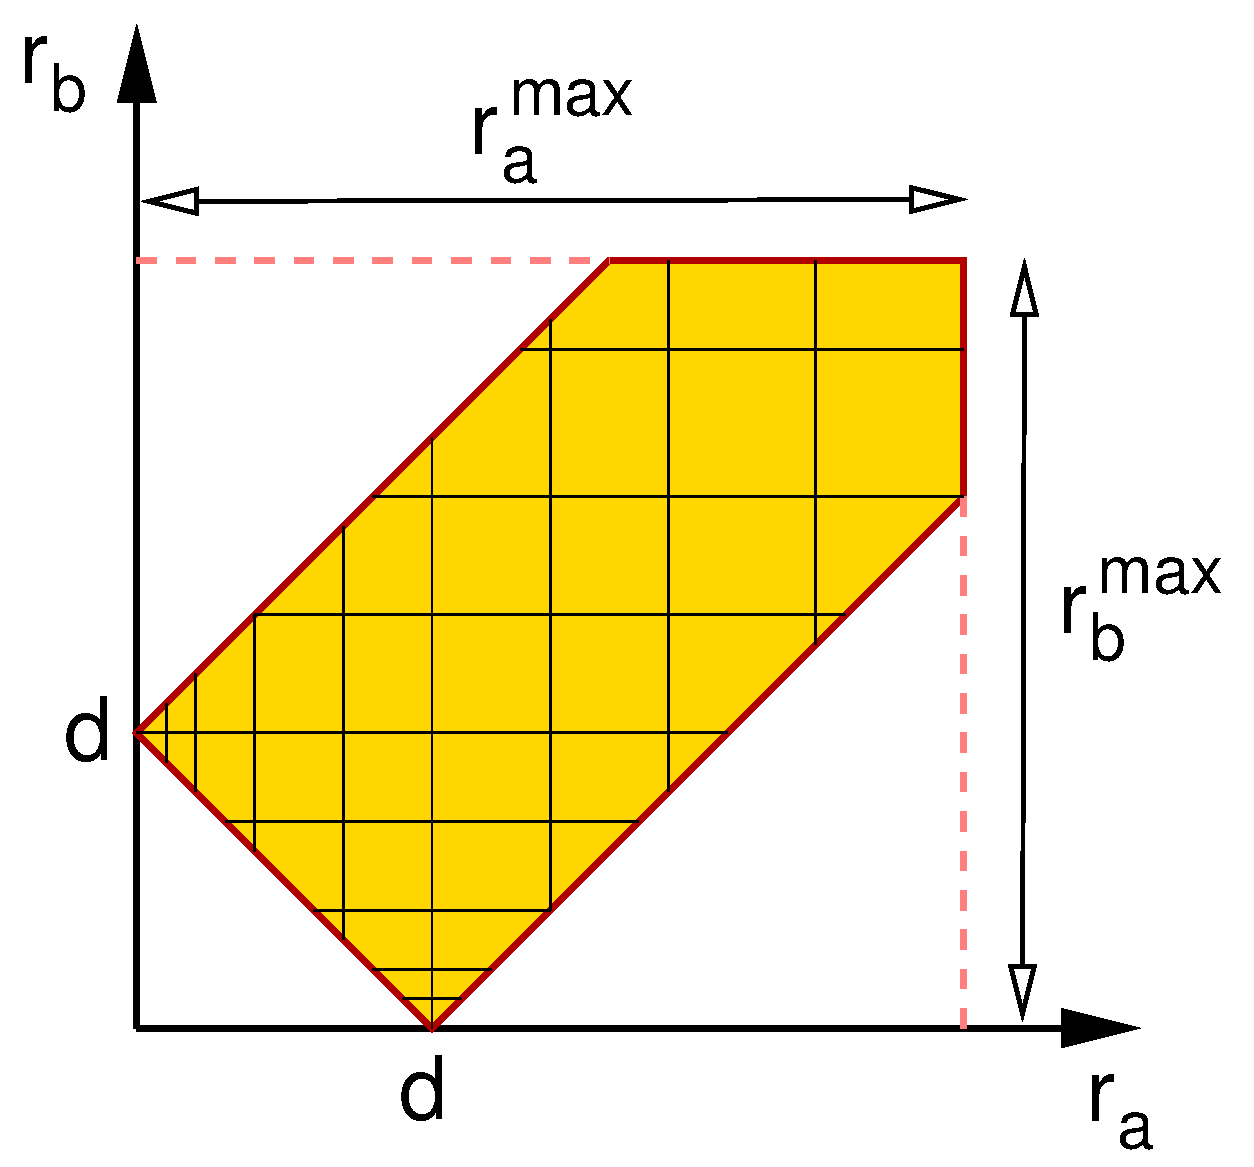
\includegraphics[width=0.5\linewidth]{Figs/Twocenterintegral/tcenter.eps}
\end{center}

This region is extended to a rectangle limited by
\begin{eqnarray*}
d\le r_a+r_b\le  max\biggl(r_a^{\text{max}},r_b^{\text{max}}\biggr)
\qquad\text{and}\qquad
-d\le r_a-r_b\le d
\end{eqnarray*}



Often the \textbf{prolate spheroidal coordinate system} \index{prolate
  spheroidal coordinate system} is introduced with the variables
\begin{eqnarray*}
\zeta(r_a,r_b)&=&\frac{1}{d}(r_a+r_b)=x_a+x_b
\\
\eta(r_a,r_b)&=&\frac{1}{d}(r_a-r_b)=x_a-x_b
\end{eqnarray*}
which essentially turns the integration area by $45^\circ$.


%==================================================================
\section{Integration using the adaptive algorithm}
\label{app:adaptiveintegration}
%==================================================================
For the integration we use the adaptive algorithm of van Dooren and de
Riddler\cite{vandooren76_jcomputapplmath2_207,
  genz80_jcomputapplmath6_295}

%==================================================================
\subsection{Gaussian quadrature on a square}
%==================================================================
One element of the method is the integration over an rectangle using
Gaussian quadrature of 7th and 5th order, such, that the 5th-order
algorithm uses the same positions as the 7th-order integration. The
comparison of the two integrations provides an error estimate in
addition to the integral.

This Gaussian-quadrature scheme containes 17 points for the
square\cite{genz80_jcomputapplmath6_295} $[-1,1]\otimes[-1,1]$
\begin{center}
\begin{tabular}{|c|c|c|c|c|}
\hline
$(0,0)$&$(+\lambda_2,0) $&$(+\lambda_3,0) $&$(+\lambda_4,+\lambda_4) $&$(+\lambda_5,+\lambda_5)$ \\
      &$(-\lambda_2,0) $&$(-\lambda_3,0) $&$(+\lambda_4,-\lambda_4) $&$(+\lambda_5,-\lambda_5)$ \\
      &$(0,+\lambda_2) $&$(0,+\lambda_3) $&$(-\lambda_4,+\lambda_4) $&$(-\lambda_5,+\lambda_5)$ \\
      &$(0,-\lambda_2) $&$(0,-\lambda_3) $&$(-\lambda_4,-\lambda_4) $&$(-\lambda_5,-\lambda_5)$ \\
\hline
$w_1   $&$ w_2           $&$    w_3        $&$     w_4                $&$     w_5$ \\
\hline
$w'_1   $&$ w'_2           $&$    w'_3        $&$     w'_4                $&$0$ \\
\hline
\end{tabular}
\end{center}
The weights sum up to four, the total area of the square. The weights
$w_i$ refer to the 7th order scheme, and the weights $w'_i$ refer to
the fifth-order scheme. 

The values are
\begin{center}
\begin{tabular}{|c|c|c|c|c|}
\hline
$\lambda_1$ &$\lambda_2$ &$\lambda_3$ &$\lambda_4$ &$\lambda_5$ \\
\hline
            &$\sqrt{9/70}$ &$\sqrt{9/10}$ &$\sqrt{9/10}$ &$\sqrt{9/19}$ \\
\hline
\hline
$w_1$ &$w_2$ &$w_3$ &$w_4$ &$w_5$ \\
\hline
-15264/19683 & 11760/19683 & 4080/19683 &800/19683 & 6859/19683\\
\hline
\hline
$w'_1$ &$w'_2$ &$w'_3$ &$w'_4$ &$w'_5$ \\
\hline
-3884/729 & 1470/729 & 130/729 & 100/729 & 0\\
\hline
\end{tabular}
\end{center}

%==================================================================
\subsection{Refining the grid}
%==================================================================
Once the integral of a square is obtained, the error estimate tells us
whether, we need to refine the grid by bisecting the square in use.

We need the information on which of the two ways of bisecting the
square is more promising. For this purpose we use the result from the
weighted sums according to the description.
\begin{center}
\begin{tabular}{|l|c|c|c|c|c|}
\hline
points 1st direction &$(-\lambda_2,0)$ & $(-\lambda_3,0)$ & $(0,0)$ & $(\lambda_3,0)$ & $(\lambda_2,0)$ \\
points 2nd direction &$(0,-\lambda_2)$ & $(0,-\lambda_3)$ & $(0,0)$ & $(0,\lambda_3)$ & $(0\lambda_2)$ \\
\hline
weights &1 & $-\left(\frac{\lambda_2}{\lambda_3}\right)^2$ &
$-2+2\left(\frac{\lambda_2}{\lambda_3}\right)^2$ & $-\left(\frac{\lambda_1}{\lambda_3}\right)^2$ &1\\ 
\hline
\end{tabular}
\end{center}
The direction with the larger absolute value is the next to be
bisected.

The rectangles are kept on an ordered stack, where the rectangles are
ordered according to the size of the predicted error. The top
rectangle with the largest error is replaced by two rectangles
covering the same area.  The rectangle with the larger error is
incorporated into the correct position starting from the top of the
stack and proceeding until its error is larger than the next on the
stack. Similarly, the rectangle with the smaller error is placed into
the correct position starting from the bottom of the stack.  For each
bisected integral the stack grows by one segment.



The value of the integral and the estimated total error is updated by
subtracting the contributions from the removed rectangle and by adding
the the values and error estimates for the two new rectangles.

======

To obtain the value of the integrand for a point in the 2-dimensional
square $[-1,1]\times[-1,1]$, we use the variable transform
\begin{eqnarray*}
\left(\begin{array}{c}r_a\\r_b\end{array}\right)
=\left(\begin{array}{c}d\\0\end{array}\right)
+\left(\begin{array}{c}r_x\\r_x\end{array}\right)\frac{1+p_1}{2}
+\left(\begin{array}{c}-d\\d\end{array}\right)\frac{1+p_2}{2}
\end{eqnarray*}
where $r_x=\max(r_a^{max},r_b^{max})$

$r_x$ is obtained by the condition that the rectangle shall cover the
complete area of points with $r_a<r_a^{max}$ and $r_b< r_b^{max}$.
Let us determine the values for $(p_1,p_2)$ that correspond to $(r_a,r_b)$.
We obtain
\begin{eqnarray*}
r^{max}_a=d+r_x\frac{1+p_1}{2}-d\frac{1+p_2}{2}
&\qquad\text{and}\qquad&
r^{max}_b=r_x\frac{1+p_1}{2}+d\frac{1+p_2}{2}
\\
\Rightarrow
r^{max}_a+r^{max}_b-d=r_x\underbrace{(1+p_1)}_{<2}
&\qquad\text{and}\qquad&
r^{max}_b-r^{max}_a+d=d(1+p_2)
\\
\Rightarrow
r_x=\frac{r^{max}_a+r^{max}_b-d}{2}
&\qquad\text{and}\qquad&
p_2=\frac{r^{max}_b-r^{max}_a}{d}
\end{eqnarray*}
By inspection we observe that there are situations where $r_x$ can be
chosen smaller. This is the case when the value of the resulting $p_2$
coordinate falls out of the allowed range, i.e. when
$|r^{max}_b-r^{max}_a|>d$.




%===============================================================================
\section{Long-range charge-charge term}
%===============================================================================
Let us consider the Coulomb interaction of two non-overlapping charge
distributions $\rho^{(A)}(\vec{r})$ and $\rho^{(B)}(\vec{r})$.
\begin{eqnarray*}
V(\vec{d})&=& \int d^3r\int d^3r'\frac{e^2\rho^{(A)}(\vec{r})\rho^{(B)}(\vec{r'}-\vec{e}_z d)}
{4\pi\epsilon_{0}|\vec{r}-\vec{r'}|}
\end{eqnarray*}

Wir verwenden die Zerlegung der Poisson Gleichung in
Kugelflaechenfunktionen, wa fuer den fernbereich das Potential
\begin{eqnarray*}
v(\vec{r})&=&\int d^3r'\frac{e^2\rho^{(A)}(\vec{r'})}
{4\pi\epsilon_{0}|\vec{r}-\vec{r'}|}
\\
&=&\sum_L \frac{4\pi}{2\ell+1} \frac{e^2}{4\pi\epsilon_0} 
\underbrace{\biggl[\int d^3r\; \rho(\vec{r}) r^{\ell} Y_L(\vec{r})\biggr]}_{Q^{(A)}_L}
\frac{1}{|\vec{r}|^{\ell+1}}Y_L(\vec{r})
\end{eqnarray*}

\begin{eqnarray*}
V(\vec{d})&=& 
\frac{e^2}{4\pi\epsilon_0} \sum_L \frac{4\pi Q_L^{(A)}}{2\ell+1} 
\int d^3r \frac{1}{|\vec{r}|^{\ell+1}}Y_L(\vec{r})\rho^{(B)}(\vec{r'}-\vec{e}_z d)
\\
\text{with}\qquad &&
Q_L^{(A)}\defas\int d^3r\; \rho^{(A)}(\vec{r}) r^{\ell} Y_L(\vec{r})
\end{eqnarray*}

Next we use the decomposition of Hankel function into
offsite-Besselfunctions for $\kappa=0$.
\begin{eqnarray*}
\underbrace{(2\ell-1)!! \frac{1}{|\vec{r}|^{\ell+1}}Y_L(\vec{r})}_{H_L(\vec{r})}&=&
-\sum_{L'}
\underbrace{
\biggl[\frac{1}{(2\ell'+1)!!} |\vec{r}-\vec{R}|^{\ell'} Y_{L'}(\vec{r}-\vec{R})\biggr]
}_{J_{L'}(\vec{r}-\vec{R})}
\\
&&
\times\underbrace{
\biggl[-4\pi\sum_{L''}\frac{(2\ell''-1)!!}{|\vec{R}|^{\ell''+1}}Y_{L''}(\vec{R})C_{L,L',L''}
(-1)^{\ell'}\delta_{\ell+\ell'-\ell''}\biggr]
}_{S^\dagger_{R,L'0,L}}
\\
\frac{1}{|\vec{r}|^{\ell+1}}Y_L(\vec{r})&=&
\sum_{L'}
\biggl[|\vec{r}-\vec{R}|^{\ell'} Y_{L'}(\vec{r}-\vec{R})\biggr]
\\
&&
\times
\biggl[\sum_{L''}\delta_{\ell+\ell'-\ell''}C_{L,L',L''}
\frac{(-1)^{\ell'}4\pi(2\ell''-1)!!}{(2\ell-1)!!(2\ell'+1)!!}
\frac{1}{|\vec{R}|^{\ell''+1}}Y_{L''}(\vec{R})
\biggr]
\end{eqnarray*}
The double factorial is defined as
\begin{eqnarray*}
n!!=\begin{cases}
1 & \text{for $n=-1,0$}\\
1\cdot3\cdot 5\cdots n & \text{for $n>0$ odd}\\
2\cdot4\cdot 6\cdots n & \text{for $n>0$ even}
\end{cases}
\end{eqnarray*}


\begin{eqnarray*}
V(d)&=& 
\frac{e^2}{4\pi\epsilon_0} \sum_L \frac{4\pi Q_L^{(A)}}{2\ell+1} 
\int d^3r \frac{1}{|\vec{r}|^{\ell+1}}Y_L(\vec{r})\rho^{(B)}(\vec{r'}-\vec{e}_z d)
\\
&=&
\frac{e^2}{4\pi\epsilon_0} \sum_{L,L'} \frac{4\pi Q_L^{(A)}}{2\ell+1} 
\biggl[\sum_{L''}\delta_{\ell+\ell'-\ell''}C_{L,L',L''}
\frac{(-1)^{\ell'}4\pi(2\ell''-1)!!}{(2\ell-1)!!(2\ell'+1)!!}
\frac{1}{|\vec{d}|^{\ell''+1}}Y_{L''}(\vec{e}_z)
\biggr]
\\
&&\times
\int d^3r\;|\vec{r}-\vec{e}_zd|^{\ell}Y_{L'}(\vec{r}-\vec{e}_zd)\rho^{(B)}(\vec{r'}-\vec{e}_z d)
\\
&=&
\frac{e^2}{4\pi\epsilon_0} \sum_{L,L'} \frac{4\pi Q_L^{(A)}Q_{L'}^{(B)}}{2\ell+1} 
\biggl[\sum_{L''}\delta_{\ell+\ell'-\ell''}C_{L,L',L''}
\frac{(-1)^{\ell'}4\pi(2\ell''-1)!!}{(2\ell-1)!!(2\ell'+1)!!}
\frac{1}{|\vec{d}|^{\ell''+1}}Y_{L''}(\vec{e}_z)
\biggr]
\\
&=&
\frac{e^2}{4\pi\epsilon_0} \sum_{L,L'} \frac{4\pi Q_L^{(A)}Q_{L'}^{(B)}}{2\ell+1} 
\biggl[C_{L,L',\ell+\ell',m=0}
\frac{(-1)^{\ell'}4\pi(2\ell+2\ell'-1)!!}{(2\ell-1)!!(2\ell'+1)!!}
\frac{1}{|\vec{d}|^{\ell+\ell'+1}}Y_{\ell+\ell',m=0}(\vec{e}_z)
\biggr]
\\
&=&
\frac{e^2}{4\pi\epsilon_0} \sum_{L,L'} \frac{ Q_L^{(A)}Q_{L'}^{(B)}}{|\vec{d}|^{\ell+\ell'+1}}
\biggl[C_{L,L',\ell+\ell',m=0}
\frac{(-1)^{\ell'}(4\pi)^2(2\ell+2\ell'-1)!!}{((2\ell+1)!!(2\ell'+1)!!}
Y_{\ell+\ell',m=0}(\vec{e}_z)
\biggr]
\end{eqnarray*}

If we conly consider monopoles and dipoles, we can use
$\bar{Y}_1(\vec{e}_x)=\frac{1}{\sqrt{4\pi}}$,
  $\bar{Y}_3(\vec{e}_z)=\sqrt{\frac{3}{4\pi}}$ and
  $\bar{Y}_7(\vec{e}_z)=\sqrt{\frac{5}{4\pi}}$.
The Gaunt coefficients needed for Monopole and dipole moments oriented along the z-direction are
$C_{sss}$, $C_{sp_zp_z}$, $C_{p_xp_x,d_{3z^2-r^2}}$,$C_{p_yp_y,d_{3z^2-r^2}}$,$C_{p_zp_z,d_{3z^2-r^2}}$.
With
\begin{eqnarray*}
\bar{Y}_s\bar{Y}_{L}&=&\frac{1}{\sqrt{4\pi}}\bar{Y}_L=C_{szz}\bar{Y}_L\qquad\Rightarrow C_{sss}=C_{sp_zp_z}=\frac{1}{\sqrt{4\pi}}
\end{eqnarray*}

\begin{eqnarray*}
\bar{Y}_5&=&\sqrt{\frac{15}{16\pi}}\frac{x^2-y^2}{\vec{r}^2}
=\sqrt{\frac{15}{16\pi}}\frac{4\pi}{3}(Y_{p_x}^2-Y_{p_y}^2)
\\
\bar{Y}_7&=&\sqrt{\frac{5}{16\pi}}\frac{3z^2-\vec{r}^2}{\vec{r}^2}=
\sqrt{\frac{5}{16\pi}}\frac{4\pi}{3}(2Y_{p_z}^2-Y_{p_x}^2-Y_{p_y}^2)
\\
\bar{Y}_0&=&\frac{1}{\sqrt{4\pi}}\frac{x^2+y^2+z^2}{\vec{r}^2}
=\sqrt{\frac{4}{16\pi}}\frac{4\pi}{3}(Y_{p_x}^2+Y_{p_y}^2+Y_{p_z}^2)
\\
\bar{Y}_{p_z}^2&=&\frac{3}{4\pi}\frac{1}{3}\biggl(\sqrt{\frac{16\pi}{4}}\bar{Y}_0+\sqrt{\frac{16\pi}{5}}\bar{Y}_7\biggr)
=\sqrt{\frac{1}{4\pi}}\bar{Y}_0+\sqrt{\frac{1}{5\pi}}\bar{Y}_7
\\
\Rightarrow \bar{C}_{p_zp_zd_{3z^2-r^2}}&=&\frac{1}{\sqrt{5\pi}}
\\
\bar{Y}_{p_x}^2
&=&\frac{3}{4\pi}\frac{1}{6}
\biggl(2\sqrt{\frac{16\pi}{4}}\bar{Y}_0-\sqrt{\frac{16\pi}{5}}\bar{Y}_7+3\sqrt{\frac{16\pi}{15}}\bar{Y}_5\biggr)
=
\sqrt{\frac{1}{4\pi}}\bar{Y}_0-\sqrt{\frac{1}{20\pi}}\bar{Y}_7+\sqrt{\frac{3}{20\pi}}\bar{Y}_5
\\
\Rightarrow \bar{C}_{p_xp_xd_{3z^2-r^2}}&=&\bar{C}_{p_yp_yd_{3z^2-r^2}}=-\frac{1}{\sqrt{20\pi}}
\end{eqnarray*}


\begin{eqnarray*}
V(d)&=&
\frac{e^2}{4\pi\epsilon_0} \sum_{L,L'} \frac{ Q_L^{(A)}Q_{L'}^{(B)}}{|\vec{d}|^{\ell+\ell'+1}}
\biggl[C_{L,L',\ell+\ell',m=0}
\frac{(-1)^{\ell'}(4\pi)^2(2\ell+2\ell'-1)!!}{((2\ell+1)!!(2\ell'+1)!!}
Y_{\ell+\ell',m=0}(\vec{e}_z)
\biggr]
\\
&=&
\frac{e^2}{4\pi\epsilon_0}\biggl\lbrace 
\frac{ Q_s^{(A)}Q_{s}^{(B)}}{|\vec{d}|}\biggl[\frac{1}{\sqrt{4\pi}}(4\pi)^2\frac{1}{\sqrt{4\pi}}\biggr]
\\
&+&\frac{ Q_s^{(A)}Q_{p_z}^{(B)}}{|\vec{d}|^{2}}
\biggl[\frac{1}{\sqrt{4\pi}}\frac{(-1)(4\pi)^2}{3}\sqrt{\frac{3}{4\pi}}\biggr]
+\frac{ Q_{p_z}^{(A)}Q_{s}^{(B)}}{|\vec{d}|^{2}}
\biggl[\frac{1}{\sqrt{4\pi}}\frac{(4\pi)^2}{3}\sqrt{\frac{3}{4\pi}}\biggr]
\\
&+&\frac{ Q_{p_z}^{(A)}Q_{p_z}^{(B)}}{|\vec{d}|^3}\biggl[\frac{1}{\sqrt{5\pi}}(4\pi)^2\frac{(-1)3}{3\cdot3}
\sqrt{\frac{5}{4\pi}}\biggr]
\\
&+&\frac{ Q_{p_x}^{(A)}Q_{p_x}^{(B)}+Q_{p_y}^{(A)}Q_{p_y}^{(B)}}{|\vec{d}|^3}
\biggl[-\frac{1}{\sqrt{20\pi}}(4\pi)^2\frac{(-1)3}{3\cdot3}
\sqrt{\frac{5}{4\pi}}\biggr]
\\
&=&
\frac{e^2}{4\pi\epsilon_0}\biggl\lbrace 
\frac{ Q_s^{(A)}Q_{s}^{(B)}}{|\vec{d}|} 4\pi
+\frac{Q_{p_z}^{(A)}Q_{s}^{(B)}- Q_s^{(A)}Q_{p_z}^{(B)}}{|\vec{d}|^{2}}
\frac{4\pi}{\sqrt{3}} 
\\
&+&\frac{ Q_{p_z}^{(A)}Q_{p_z}^{(B)}}{|\vec{d}|^3}\biggl( -4\pi\frac{2}{3}\biggr)
+\frac{ Q_{p_x}^{(A)}Q_{p_x}^{(B)}+Q_{p_y}^{(A)}Q_{p_y}^{(B)}}{|\vec{d}|^3}
\biggl[\frac{1}{3}(4\pi)\biggr]
\\
&=&
4\pi\cdot\frac{e^2}{4\pi\epsilon_0}\biggl\lbrace 
\frac{ Q_s^{(A)}Q_{s}^{(B)}}{|\vec{d}|}
+\frac{1}{\sqrt{3}}\frac{Q_{p_z}^{(A)}Q_{s}^{(B)}}{d^2}- \frac{1}{\sqrt{3}}\frac{Q_s^{(A)}Q_{p_z}^{(B)}}{d^2}
\\
&&-\frac{2}{3}\frac{ Q_{p_z}^{(A)}Q_{p_z}^{(B)}}{|\vec{d}|^3}
+\frac{1}{3}\frac{ Q_{p_x}^{(A)}Q_{p_x}^{(B)}}{|\vec{d}|^3}
+\frac{1}{3}\frac{ Q_{p_y}^{(A)}Q_{p_y}^{(B)}}{|\vec{d}|^3}\biggr\rbrace
\end{eqnarray*}

This expression can also be divided into rotationally invariant
repulsive terms and axial terms that may be attractive or repulsive.
\begin{eqnarray*}
V(d)&=&
4\pi\cdot\frac{e^2}{4\pi\epsilon_0}\biggl\lbrace 
\frac{ Q_s^{(A)}Q_{s}^{(B)}}{|\vec{d}|}+\frac{1}{3}\frac{Q_{p_x}^{(A)}Q_{p_x}^{(B)}+Q_{p_y}^{(A)}Q_{p_y}^{(B)}+Q_{p_z}^{(A)}Q_{p_z}^{(B)}
}{|\vec{d}|^3}
\\
&&\hspace{1.7cm}
-\frac{1}{\sqrt{3}}\frac{Q_s^{(A)}Q_{p_z}^{(B)}-Q_{p_z}^{(A)}Q_{s}^{(B)}}{d^2}
-\frac{ Q_{p_z}^{(A)}Q_{p_z}^{(B)}}{|\vec{d}|^3}
\biggr\rbrace
\end{eqnarray*}

Now we introduce the definition for the dipole
\begin{eqnarray*}
q&=&\sqrt{4\pi}Q_s=\sqrt{4\pi}\int d^3r\;\rho(\vec{r})Y_s(\vec{r})=\int d^3r\;\rho(\vec{r})
\\
\vec{D}&=&\sqrt{\frac{4\pi}{3}}\left(\begin{array}{c}Q_{p_x}\\Q_{p_y}\\Q_{p_z}\end{array}\right)
=\sqrt{\frac{4\pi}{3}}\int d^3r\;\rho(\vec{r})|\vec{r}|
\left(\begin{array}{c}Y_{p_x}\\Y_{p_y}\\Y_{p_z}\end{array}\right)
=\sqrt{\frac{4\pi}{3}}\int d^3r\;\rho(\vec{r})\sqrt{\frac{3}{4\pi}}\vec{r}
=\int d^3r\;\rho(\vec{r})\vec{r}
\end{eqnarray*}
so that
\begin{eqnarray*}
V(d)&=&
\frac{e^2}{4\pi\epsilon_0}\biggl\lbrace 
\frac{ q^{(A)}q^{(B)}}{|\vec{d}|}+\frac{\vec{D}^{(A)}\vec{D}^{(B)}}{|\vec{d}|^3}
-\frac{q^{(A)}\vec{D}^{(B)}\vec{e}_z-\vec{D}^{(A)}\vec{e}_zq^{(B)}}{d^2}
-\frac{ 3(\vec{e}_z\vec{D}^{(A)})(\vec{e}_z\vec{D}^{(B)})}{|\vec{d}|^3}
\biggr\rbrace
\end{eqnarray*}



%=====================================================================
\chapter{Screening length}
%=====================================================================
In the random-phase approximation of the free electron gas the coulomb
interaction in the exchange energy is replaced by a Yukawa potential.
\begin{eqnarray}
v_{\text{Yukawa}}(\vec{r})
=\frac{e^2}{4\pi\epsilon_0|\vec{r}|}
\e{-\lambda|\vec{r}|}
\end{eqnarray}
In Fourier space the Yukawa potential 
\begin{eqnarray}
v_{\text{Yukawa}}(\vec{r})=\int \frac{d^3G}{(2\pi)^3}\;
  \frac{e^2}{4\pi\epsilon_0}\frac{4\pi}{G^2+\lambda^2}
\end{eqnarray}

The potential can also be expressed in terms of a $G$-dependent
dielectric constant.
\begin{eqnarray}
\epsilon_r^{-1}(\vec{G})=\frac{\vec{G}^2}{\vec{G}^2+\lambda^2}
\end{eqnarray}

This can be compared with the slide ``An analogy between GW anmd
hybrid functionals'' in
\url{https://www.nersc.gov/assets/Uploads/VASP-lecture-RPA.pdf}

I am using one data pair ($\epsilon_r^{-1}=0.5$ for $G=2$~$\AA^{-1}$)
to arrive at $\lambda=2 a_0^{-1}$ or $r_{screen}=0.5$~$a_0$.





%=====================================================================
\subsubsection{HSE06}
%=====================================================================
The HSE06 functional is the prototypical range-separated hybrid
density functional. A fortran implementation can be be found in the
Thesis of Jochen Heyd, which can be found on the internet.  (Caution:
In the HSE03 functional different screening parameters have been used
for the Fock term and the subtraction of the PBE exchange.)

(See in \url{Codes/Holefunction/src/hsfx.f90})

Krukau\cite{krukau06_jcp125_224106} finds that energies depend little
on the range, if the range for the double counting and the screened
Fock term are similar in the range $5~a_B<r_{screen}<\infty$. This
indicates that it is important to include the first nearest and
next-nearest neighbor shells.

Krukau\cite{krukau06_jcp125_224106} shows in his table VIII that band
gaps become better with increasing range, and that this improvement
depends on the fock admixture, while it is fairly independent of the
range in the double counting.


This suggests that we should use the same $\alpha_{Fock}=0.25$ as
HSE06 to get the correct band gaps. The screening length can be chosen
smaller. \textcolor{red}{Our double counting term is not consistent
  the off-site terms and differs from that of HSE06.}



%=====================================================================
\subsubsection{Test for Si}
%=====================================================================

\begin{center}
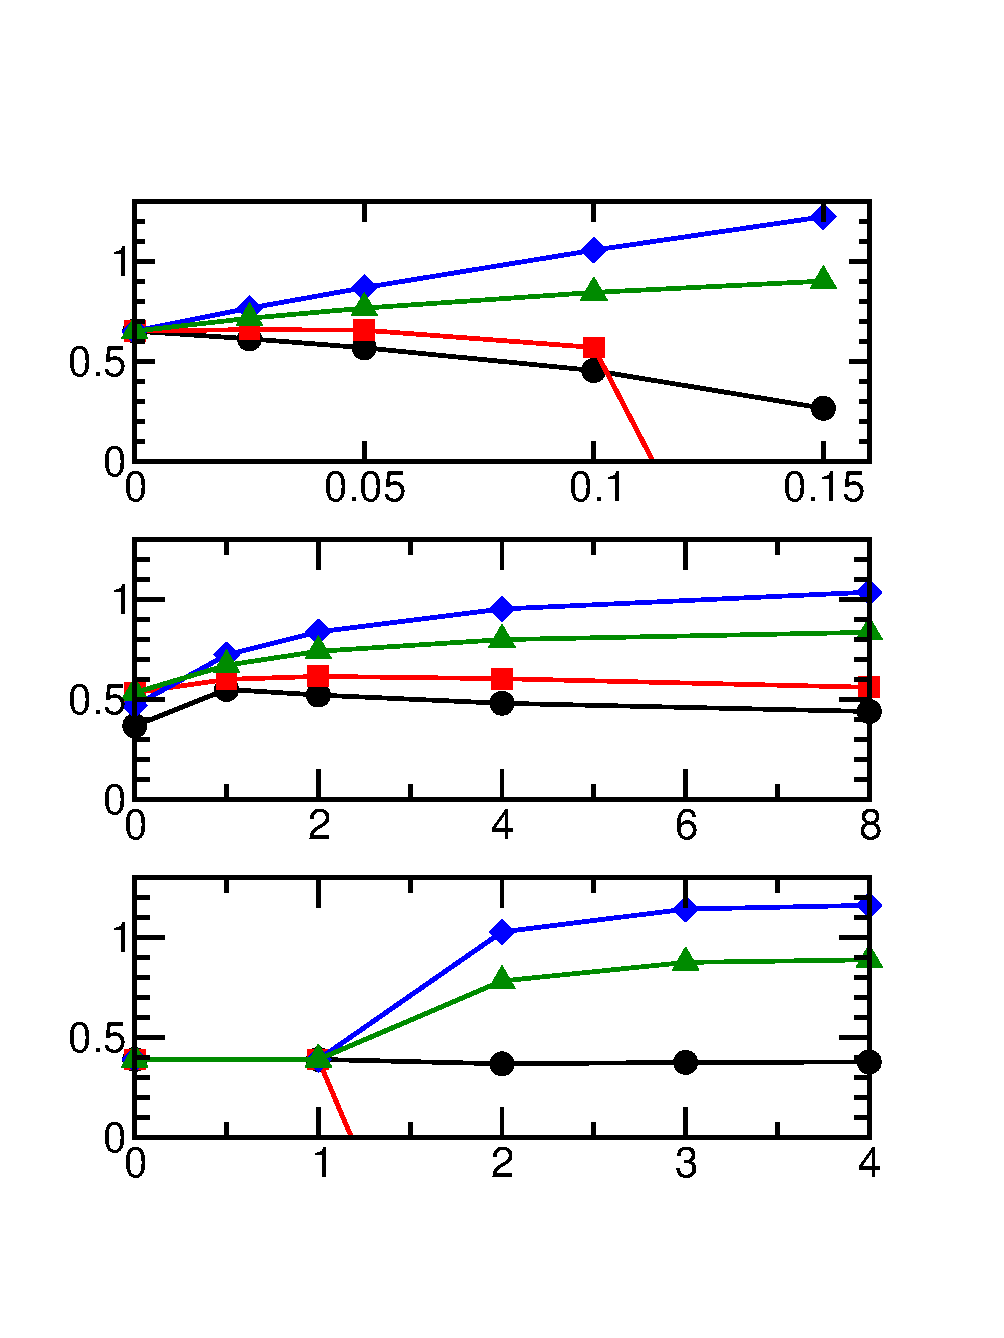
\includegraphics[width=0.5\linewidth]{Figs/sitests1}
\end{center}
Band gap of silicon as function of (top) the Hartree Fock weight, (2)
the screening length in \AA and (bottom)the cutoff radius for the
neighborlist. The standard values are 0.125 for the Hartree-Fock
weight, 3~\AA for the screening length and 3~$r_{cov}$=3.33~\AA for
the radius of the neighbor list. PBE0r (local terms only) black
spheres, PBE0r+NDDO red squares, PBE0r+NDDO+31 (blue diamonds) and
PBE0r+31 (green triangles).

\begin{itemize}
\item PBE0r: with increasing $\alpha_{fock}$, the s-bands are shifted
  down in energy.  The $ss\sigma$ hopping seems to be reduced (The
  band width of s-band is narrower).  The conduction band has a lot of
  s-character. Thus the s-band shifts downward with increasing
  Fock-weight.
%
\item 31: The $ss\sigma$ hopping is drastically increased.(band width
  of s-band is larger)
%
\item NDDO for $\alpha_{fock}>0.1$ develops ghost states
\end{itemize}

I changed $K2=-1$ so that the tails of the local orbital have a
kinetic energy of 1~Ry=0.5~H. The screening length has been set to
$3~\AA$ and the cutoff radius has been set to three times the sum of
covalent radii, i.e. 6~\AA.





%=====================================================================
\chapter{Changelog, Bugfixes}
%=====================================================================
\begin{itemize}
\item the core-valence exchange contribution differs from the old
  version, because it also includes the projection on the phidot
  functions.
%
\item there has been a bug in \verb|lmto$screen|, which has been fixed
  with version 3. It may be better to rewrite all structure constants
  routines with the transposed structure constants.
%
\item in \verb|lmto$makestructureconstants|, the structure constants
  have not been calculated because the parallelzation was wrong.  in
  13403f6.
\begin{verbatim}
-       IF(MOD(IAT1-1,NTASKS).NE.THISTASK-1) THEN
+       IF(MOD(IAT1-1,NTASKS).eq.THISTASK-1) THEN
\end{verbatim}
%
\end{itemize}


\clearpage
\bibliographystyle{unsrtnat} \bibliography{../all}
\end{document}  
